% !TeX encoding = UTF-8
% !TeX spellcheck = en_UK

%% https://en.wikibooks.org/wiki/LaTeX/Document_Structure
\documentclass[]{clmthesis}

%% https://en.wikibooks.org/wiki/LaTeX/Modular_Documents
% !TeX root = ../mthesis.tex
% !TeX encoding = UTF-8
% !TeX spellcheck = en_US


%% == LaTeX ============================================================= %%
%% https://en.wikibooks.org/wiki/LaTeX
%% ====================================================================== %%


%% -- 2.4 Colors -------------------------------------------------------- %%
%% https://en.wikibooks.org/wiki/LaTeX/Colors
\usepackage[usenames,dvipsnames,svgnames,table]{xcolor}
% !TeX encoding = UTF-8
% !TeX spellcheck = en_US

%% https://en.wikibooks.org/wiki/LaTeX/Colors

%% color definitions

% \colorlet{col:a}{Fuchsia}
% \colorlet{col:b}{Blue}
\colorlet{colG}{Gray}
\colorlet{colO}{Orange}
\colorlet{colHi}{Green}
\colorlet{colLo}{Red}
\colorlet{colNa}{Gray}
\colorlet{colN}{Blue}
\colorlet{colEm}{RoyalBlue}
\colorlet{colMAXIMAL}{Violet}
\colorlet{colSTRICTLY}{RoyalBlue}

%% PAINT IT BLACK =========
% \colorlet{col:a}{black}
% \colorlet{col:b}{black}
% \colorlet{colG}{black}
% \colorlet{colO}{black}
% \colorlet{colHi}{black}
% \colorlet{colLo}{black}
% \colorlet{colNa}{black}
% \colorlet{colN}{black}
% \colorlet{colEm}{black}
% \colorlet{colMAXIMAL}{black}
% \colorlet{colSTRICTLY}{black}

%\newcommand{\colA}{\color{col:a}}	% example a
%\newcommand{\colB}{\color{col:b}}	% example b
\newcommand{\colG}{\color{colG}}	% neutral
\newcommand{\colO}{\color{colO}}	% old
\newcommand{\colN}{\color{colN}}	% new
\newcommand{\colHi}{\color{colHi}}	% hi, true
\newcommand{\colLo}{\color{colLo}}	% lo, false
\newcommand{\colNA}{\color{colNa}}	% not available
\newcommand{\colEm}{\color{colEm}}

%\newcommand{\colMax}{\color{colMax}}	% maximal
%\newcommand{\colSmx}{\color{colSmx}}	% strictly maximal

%\newcommand{\MYa}{\color{Fuchsia}}
%\newcommand{\MYb}{\color{Blue}}
%\newcommand{\MYg}{\color{Gray}}
%\newcommand{\MYo}{\color{Orange}}
%
%\newcommand{\MYhi}{\color{Green}}
%\newcommand{\MYlo}{\color{Red}}
%\newcommand{\MYna}{\color{Gray}}
%
%\newcommand{\MYA}[1]{{\MYa#1}}
%\newcommand{\MYB}[1]{{\MYb#1}}
%\newcommand{\MYG}[1]{{\MYg#1}}
%\newcommand{\MYO}[1]{{\MYo#1}}
%
%\newcommand{\MYHI}[1]{{\MYhi#1}}
%\newcommand{\MYLO}[1]{{\MYlo#1}}
%\newcommand{\MYNA}[1]{{\MYna#1}}
%
%\newcommand{\MYS}[1]{{\color{Violet}#1}}
%\newcommand{\MYM}[1]{{\color{RoyalBlue}#1}}
%
%\newcommand{\mLightning}{{\text{\Lightning}}}

%% ---------------------------------------------------------------------- %%


%% -- 2.8 Internationalization ------------------------------------------ %%
%% https://en.wikibooks.org/wiki/LaTeX/Internationalization
\usepackage[utf8x]{inputenc} 		% input
\usepackage[LGR,T1]{fontenc}	 	% output (PDF)
\usepackage[english]{babel}			% language

%% ---------------------------------------------------------------------- %%


%% -- 2.10 Tables ------------------------------------------------------- %%
% https://en.wikibooks.org/wiki/LaTeX/Tables
%% ---------------------------------------------------------------------- %%


%% -- 2.16-17 Hyperlinks ------------------------------------------------ %%
% https://en.wikibooks.org/wiki/LaTeX/Hyperlinks
% https://en.wikibooks.org/wiki/LaTeX/Labels_and_Cross-referencing
\usepackage{hyperref}
%\usepackage[xindy,toc]{glossaries}
\usepackage[toc]{glossaries}
\usepackage[]{index}
%% ---------------------------------------------------------------------- %%


%% -- 4.1-3 Mathematics ------------------------------------------------- %%
% https://en.wikibooks.org/wiki/LaTeX/Mathematics
% https://en.wikibooks.org/wiki/LaTeX/Advanced_Mathematics
\usepackage{amsmath}		
\usepackage{mathtools} 
\usepackage{amssymb}

% https://en.wikibooks.org/wiki/LaTeX/Theorems
\usepackage{amsthm}			
\usepackage{proof} 
\usepackage{bussproofs}
\usepackage{marvosym}

\usepackage{multirow}
\usepackage[makeroom]{cancel} % \(b|x)cancel(to{}){}
%\usepackage{soul}
\usepackage{pdfcomment}


\DeclareMathAlphabet{\mathpzc}{OT1}{pzc}{m}{it}	% \mathpzc
\DeclareMathAlphabet{\mathcll}{T1}{calligra}{m}{n}
%\usepackage{calrsfs}
%\DeclareMathAlphabet{\pazocal}{OMS}{zplm}{m}{n}

% !TeX encoding = UTF-8

%% ==============================================================
%% ### MY MATH ENVIRONMENTS ###

\theoremstyle{plain}
%\newtheorem{theorem}{Theorem}			% predefined in CL?
%\newtheorem{proposition}{Proposition}	% predefined in CL?
%\newtheorem{lemma}{Lemma}				% predefined in CL?
%\newtheorem*{corollary}{Corollary}		% predefined in CL?

\theoremstyle{definition}
%\newtheorem{definition}{Definition}	% predefined in CL?
\newtheorem{conjecture}{Conjecture}
%\newtheorem*{example}{Example}			% predefined in CL?
%\newtheorem{algorithm}{Algorithm}		% predefined in CL
\newtheorem{procedure}{Procedure}
\newtheorem{goal}{Goal}
\newtheorem{notation}{Notation}

\theoremstyle{remark}
\newtheorem*{remark}{Remark}			% predefined in CL?
\newtheorem*{observation}{Observation}
%\newtheorem*{note}{Note}
%\newtheorem{case}{Case}

%% ==============================================================
%% ### MY MATH DEFINITIONS ###

% math alphabets

\DeclareMathAlphabet{\mathpzc}{OT1}{pzc}{m}{it}	% \mathpzc
\DeclareMathAlphabet{\mathcll}{T1}{calligra}{m}{n}

% math operators

\DeclareMathOperator{\arity}{arity}		% arity of a symbol

\DeclareMathOperator{\var}{\mathpzc{Vars}}			% variables of a term
\DeclareMathOperator{\fun}{\mathpzc{Funs}}			% function symbols of a term
\DeclareMathOperator{\pos}{\mathpzc{Pos}}			% positions in a term
\DeclareMathOperator{\posT}{\mathpzc{{t-}Pos}}			% positions in a term
\DeclareMathOperator{\posS}{\mathpzc{Pos^F}}
%\DeclareMathOperator{\pos}{\mathcal{P}\mathsf{os}}
\DeclareMathOperator{\fvar}{\mathpzc{Fvars}}
\DeclareMathOperator{\bvar}{\mathpzc{Bvars}}

%\DeclareMathOperator{\var}{\mcV}			% variables of a term
%\DeclareMathOperator{\fun}{\mcFf}			% function symbols of a term
%\DeclareMathOperator{\pos}{\mathcal{P}\mathsf{os}}			% positions in a term

%\DeclareMathOperator{\T}{T}
	\DeclareMathOperator{\domain}{dom}			% domain of an assignment
	\DeclareMathOperator{\range}{rng}		% range of an assignment
	\DeclareMathOperator{\image}{img}			% image of an assignment
\DeclareMathOperator{\mgu}{mgu}			% most general unifier
%\DeclareMathOperator{\wgt}{W\!}
\DeclareMathOperator{\sel}{sel}			% selection function
%\DeclareMathOperator{\mul}{mul}
%\DeclareMathOperator{\add}{add}
\DeclareMathOperator{\head}{head}
\DeclareMathOperator{\tail}{tail}
\DeclareMathOperator{\length}{length}


%\DeclareMathOperator{\UNIF}{unifiable}
%\DeclareMathOperator{\INST}{instance}
%\DeclareMathOperator{\GNRL}{generalization}
%\DeclareMathOperator{\VRNT}{variant}
%\DeclareMathOperator{\PSTR}{pstr}

\DeclareMathOperator{\subterms}{\mathpzc{Subterms}}	
\DeclareMathOperator{\termsize}{size}
\DeclareMathOperator{\symbols}{symbols}
\DeclareMathOperator{\subforms}{\mathpzc{Subforms}}	
%% ---------------------------------------------------------------------- %%


\usepackage{varioref}


%\usepackage{calc}
%\usepackage{geometry}

%% -- 4.5 Algorithms ---------------------------------------------------- %%
% https://en.wikibooks.org/wiki/LaTeX/Algorithms
%% ---------------------------------------------------------------------- %%


%% -- 4.6 Listings ------------------------------------------------------ %%
% https://en.wikibooks.org/wiki/LaTeX/Source_Code_Listings
\usepackage{listings} 
% !TeX encoding = UTF-8
% !TeX spellcheck = en_US

\lstdefinelanguage{smtlib}{
	comment={[l];},
	keywords={assert,xor, or, and},
	otherkeywords={declare-fun, set-logic},
	emph={Int,QF_LIA},
}

\lstdefinelanguage{Yices}{
	language = C,
	morekeywords={},
%	comment={[l];},
%	keywords={assert,xor, or, and},
	keywords=[2]{type_t, uint32_t, term_t},
%	emph={Int,QF_LIA},
%	otherkeywords={yices_bool_type}
}

\lstdefinelanguage{flea}{
	language = C,
%	morekeywords={},	
	%	comment={[l];},
	%	keywords={assert,xor, or, and}, 	% 
	keywords=[2]{func, var, let, protocol, associatedtype, extension},	% Swift Keywords
	keywords=[3]{String, UInt32},					% Swift data types
	keywords=[4]{type_t, uint32_t, term_t,},		% yices data types
	%%% begin yices API keywords %%%
	keywords=[5]{yices_get_type_by_name, yices_new_uninterpreted_term, yices_new_uninterpreted_type}				
	%%% end yices API keywords %%%
	%	emph={Int,QF_LIA},
	%	otherkeywords={yices_bool_type}
}

\lstset {
	backgroundcolor=\color{white},     	% choose the background color; you must add \usepackage{color} or \usepackage{xcolor}
	basicstyle=\ttfamily\footnotesize, 	% the size of the fonts that are used for the code
	breakatwhitespace=false,         	% sets if automatic breaks should only happen at whitespace
	breaklines=true,                 	% sets automatic line breaking
	caption=\lstname,
	captionpos=b,                    	% sets the caption-position to bottom
	commentstyle=\color{gray},    		% comment style
	deletekeywords={...},            	% if you want to delete keywords from the given language
	emphstyle=\color{orange},
	escapeinside={\%*}{*)},         % if you want to add LaTeX within your code
	extendedchars=true,             % lets you use non-ASCII characters; for 8-bits encodings only, does not work with UTF-8
	frame=none,		% frame=single, % adds a frame around the code
	keepspaces=true,                % keeps spaces in text, useful for keeping indentation of code (possibly needs columns=flexible)
	keywordstyle=\color{OliveGreen},      % keyword style
	keywordstyle=[2]\color{Fuchsia},
	keywordstyle=[3]\color{RedViolet},
	keywordstyle=[4]\color{RoyalBlue},	% yices data types
	keywordstyle=[5]\color{NavyBlue},	% yices api
	% language=smtlib,	%Octave,    % the language of the code
	% literate={;},
	% otherkeywords={declare-fun,set-logic,assert,xor,or,and},            % if you want to add more keywords to the set
	%morecomment=[l]{;}				% line comment
	numbers=left,                   % where to put the line-numbers; possible values are (none, left, right)
	numbersep=5pt,                  % how far the line-numbers are from the code
	numberstyle=\tiny\color{gray}, 	% the style that is used for the line-numbers
	rulecolor=\color{black},        % if not set, the frame-color may be changed on line-breaks within not-black text (e.g. comments (green here))
	showspaces=false,               % show spaces everywhere adding particular underscores; it overrides 'showstringspaces'
	showstringspaces=false,         % underline spaces within strings only
	showtabs=false,                 % show tabs within strings adding particular underscores
	stepnumber=1,                   % the step between two line-numbers. If it's 1, each line will be numbered
	stringstyle=\color{orange},     % string literal style
	tabsize=2,	                   	% sets default tabsize to 2 spaces
%	title=\lstname,                  % show the filename of files included with \lstinputlisting; also try caption instead of title,
	mathescape=true
}
	% definitions
%% ---------------------------------------------------------------------- %%


%% -- Graphics ---------------------------------------------------------- %%
% https://en.wikibooks.org/wiki/LaTeX/PGF/TikZ
\usepackage{tikz}
\documentclass{clseminar}

    \usepackage{tikz}
    \usepackage{soul}

    % \documentclass{clseminar}

    \usepackage{tikz}
    \usepackage{soul}

    % \input{../PREAMBLE/Drawings}

\begin{document}

\begin{figure}
    \begin{center}
\input{../DRAWINGS/ProperOrder}
\caption{Proper orders on terms}
    \end{center}
\end{figure}

\begin{figure}
    \begin{center}
\input{../DRAWINGS/PartialOrder}
\caption{Equivalence relation vs.~partial order}
\end{center}
\end{figure}

\end{document}

\begin{document}

\begin{figure}
    \begin{center}
\begin{tikzpicture}
    \node (defCUC) at (-4,8.5) { \( s\succ t\Rightarrow \ctx[s]\succ \ctx[t] \)};
    \node (CUC) at (-4,8) { contexts };
    \node (defCUS) at (0,8.5) { \( s\succ t\Rightarrow s\sigma\succ t\sigma \)};
    \node (CUS) at (0,8) { substitutions };

    \node (ASYM) at (4,8.5) { \( s\succ t\Rightarrow t\not\succ s \) };
    \node (ASYM) at (4,8) { asymmetric };

        \node (CL) at (-2,6) { closed under };
        \node (defIRR) at (2,6.5) { \( s\succ t\succ u\Rightarrow s\succ u \) };
        \node (IRR) at (6,6) { irreflexive };
        \node (defIRR) at (6,6.5) { \( s\nsucc s \) };
        \node (TRA) at (2,6) { transitive };

        \node (POx) at (4,4.4) { \( > \) };
        \node (PO) at (4,4) { proper order };
        \node (RWRx) at (0,4.4) { \( \rightarrow^*_\mcR \) };
        \node (RWR) at (0,4) { rewrite relation };

        \node (defSTP) at (-2,2.5) { \( \ctx\neq\ctxhole\Rightarrow \ctx[s]\succ s \) };
        \node (STP) at (-2,2) { subterm property };
        \node (RWO) at (2,2) { rewrite order };
        \node (defWF) at (8,4.5) { \( \nexists s_0(s_i\succ s_{i+1})_{i=0}^{\infty} \) };
        \node (WF) at (8,4) { well-founded };

        \node (SO) at (0,0) {simplification order};
        \node (RO) at (4,0) {reduction order};

        \node (WFO) at (6,2) { well-founded order };


        \draw[->] (CL) -- (CUC);
        \draw[->] (CL) -- (CUS);

        \draw[->] (PO) -- (IRR);
        \draw[->] (PO) -- (TRA);

        \draw[->] (RWR) -- (CL);

        \draw[->] (RWO) -- (PO);
        \draw[->] (RWO) -- (RWR);

        \draw[->] (SO) -- (STP);
        \draw[->] (RO) -- (RWO);
        \draw[->] (RO) -- (WFO);
        % \draw (RO) edge[out=0,in=-45,->] (WF);

        \draw[->] (SO) -- (RWO);
        \draw[->, dotted] (SO) -- (RO);

        \draw[->] (WFO) -- (WF);
        \draw[->] (WFO) -- (PO);

        \draw[->, dotted] (WF) -- (IRR);

        % \node (TRAIRR) at (4,7) { \( \bullet \) };
        \draw[->, dotted] (4,7) -- (ASYM);

        \draw[dotted] (TRA) edge [out=-10, in=-90] (4,7);
        \draw[dotted] (IRR) edge [out=190, in=-90] (4,7);

        \draw[->, dotted] (ASYM) -- (IRR);
        % \draw[->, dotted] (ASYM) edge [out=0, in=0] (IRR);


    \end{tikzpicture}
\caption{Proper orders on terms}
    \end{center}
\end{figure}

\begin{figure}
    \begin{center}
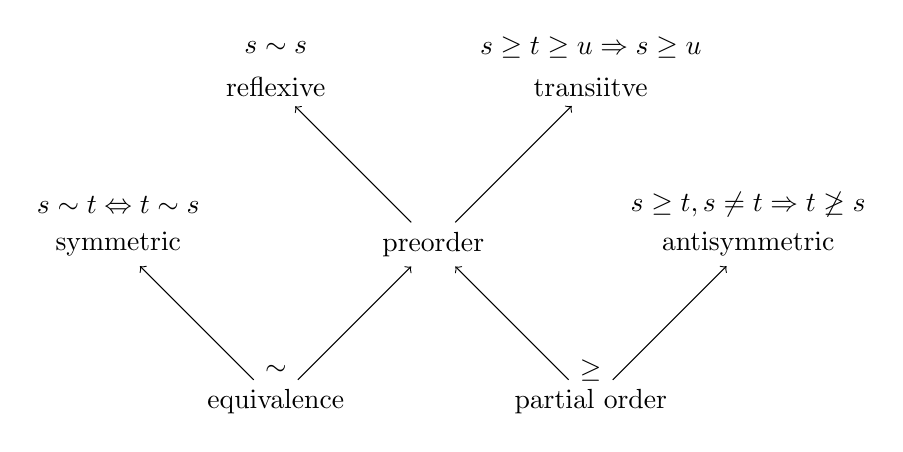
\begin{tikzpicture}
    \node (defREFLEXIVE) at (-2,2.5) { $s\sim s$ };
    \node (REFLEXIVE) at (-2,2) { reflexive };

    \node (defTRANSITIVE) at (2,2.5) { $s\geq t\geq u\Rightarrow s\geq u$ };
    \node (TRANSITIVE) at (2,2) { transiitve };

    \node (defTRANSITIVE) at (-4,0.5) { $s\sim t\Leftrightarrow t\sim s$ };
    \node (SYMMETRIC) at (-4,0) { symmetric };
    \node (PREORDER) at (0,0) { preorder };

    \node (defANTISYMMETRIC) at (4,0.5) { $s\geq t, s\neq t \Rightarrow t\not\geq s$ };
    \node (ANTISYMMETRIC) at (4,0) { antisymmetric };
    \node (SIM) at (-2,-1.6) { $\sim$ };
    \node (EQUIVALENCE) at (-2,-2) { equivalence };
    \node (GEQ) at (2,-1.6) { $\geq$ };
    \node (PARTIAL) at (2,-2) { partial order };

    \draw[->] (PREORDER) -- (REFLEXIVE);
    \draw[->] (PREORDER) -- (TRANSITIVE);

    \draw[->] (EQUIVALENCE) -- (SYMMETRIC);
    \draw[->] (EQUIVALENCE) -- (PREORDER);
    \draw[->] (PARTIAL) -- (PREORDER);
    \draw[->] (PARTIAL) -- (ANTISYMMETRIC);
\end{tikzpicture}
\caption{Equivalence relation vs.~partial order}
\end{center}
\end{figure}

\end{document}		% definitions and tikz macros
\usepackage[thinlines,thiklines]{easybmat}
%% ---------------------------------------------------------------------- %%

%% -- Macros ------------------------------------------------------------ %%
%% https://en.wikibooks.org/wiki/LaTeX/Macros
\usepackage{xspace}
% !TeX encoding = UTF-8

% shortens the definition by cases
\newcommand{\DEFINE}[3][=]{{
		\begin{gather*}
		#2 #1 \left \{
				\begin{array}{ll}
					#3
				\end{array}
		\right.
		\end{gather*}
	}}

\newcommand{\MDEFINE}[4][=]{\ensuremath{
		#2 #1 \left \{
				\begin{array}{#3}
					#4
				\end{array}
		\right.
	}}


% accepts greek as input
\newcommand{\textgreek}[1]{\begingroup\fontencoding{LGR}\selectfont#1\endgroup}

\newcommand{\tikzmark}[1]{\tikz[overlay,remember picture] \node(#1) {};}


		% complex macros
% !TeX root = ../mythesis.tex
% !TeX encoding = UTF-8

% cspell:disable

%% ==============================================================
%% ### MISC ###



%% ==============================================================
% ### provide commands
%% ==============================================================
\providecommand{\colEm}{}	% not color et all
%% ==============================================================

% math alphabets

\DeclareMathAlphabet{\mathpzc}{OT1}{pzc}{m}{it}	% \mathpzc
\DeclareMathAlphabet{\mathcll}{T1}{calligra}{m}{n}

% math operators

\DeclareMathOperator{\arity}{arity}		% arity of a symbol

\DeclareMathOperator{\var}{\mathpzc{Vars}}			% variables of a term
\DeclareMathOperator{\fun}{\mathpzc{Funs}}			% function symbols of a term
\DeclareMathOperator{\pos}{\mathpzc{Pos}}			% positions in a term
\DeclareMathOperator{\posT}{\mathpzc{{t-}Pos}}			% positions in a term
\DeclareMathOperator{\PosStr}{\mathpzc{Pos^F}}
\DeclareMathOperator{\vaPosStr}{\mathpzc{Pos^F_*}}
\DeclareMathOperator{\posV}{\mathpzc{Pos^{\!V}}}
\DeclareMathOperator{\occurs}{occurs}
\DeclareMathOperator{\fvar}{\mathpzc{Fvars}}
\DeclareMathOperator{\bvar}{\mathpzc{Bvars}}

\DeclareMathOperator{\domain}{dom}			% domain of an assignment
\DeclareMathOperator{\range}{rng}		% range of an assignment
\DeclareMathOperator{\image}{img}			% image of an assignment
\DeclareMathOperator{\IRRED}{irred}

\DeclareMathOperator{\mgu}{mgu}			% most general unifier
\DeclareMathOperator{\sel}{sel}			% selection function

%\DeclareMathOperator{\mul}{mul}
%\DeclareMathOperator{\add}{add}
\DeclareMathOperator{\head}{head}
\DeclareMathOperator{\tail}{tail}
\DeclareMathOperator{\length}{length}

\DeclareMathOperator{\UNIF}{unifiable}
\DeclareMathOperator{\INST}{instance}
\DeclareMathOperator{\GNRL}{generalization}
\DeclareMathOperator{\VRNT}{variant}
\DeclareMathOperator{\SUBS}{subsumses}
\DeclareMathOperator{\PSSTR}{substring}
\DeclareMathOperator{\PSTR}{pstr}

%\DeclareMathOperator{\subterms}{\mathpzc{Subterms}}
%\DeclareMathOperator{\termsize}{size}
%\DeclareMathOperator{\symbols}{symbols}
%\DeclareMathOperator{\subforms}{\mathpzc{Subforms}}


%\newcommand\TOP[2]{\genfrac{}{}{0pt}{}{#1}{#2}}
%\newcommand\TOPTEXT[2]{\TOP{\text{#1}}{\text{#2}}}
%\newcommand{\mygreek}[1]{\selectlanguage{polutonikogreek}#1\selectlanguage{english}}
%\newcommand{\mygreek}[1]{{\selectlanguage{polutonikogreek}#1}\selectlanguage{english}}
%\renewcommand{\mygreek}[1]{\foreignlanguage{polutonikogreek}{#1}}

%\newcommand{\iSUB}[2]{#2\!\mapsto\!#1}
%\newcommand{\BgSyntaxTree}{\usebackgroundtemplate{\transparent{0.1}\includegraphics[width=\paperwidth]{SyntaxTreeBackground.png}}}

%\newcommand{\EMPH}[1]{\emph{\textcolor{colEm}{#1}}}
\newcommand{\coloremph}[1]{\textcolor{colEm}{\emph{#1}}}


%\newcommand{\NGTPREQ}{\not\succcurlyeq}

\newcommand{\succG}{\mathrel\succ_{\!\mathtt{gr}}}
\newcommand{\succL}{\mathrel\succ_{\mathtt{L}}}
\newcommand{\succC}{\mathrel\succ_{\mathtt{C}}}

\newcommand{\disjointunion}{\mathbin{\dot\cup}}
\newcommand{\limp}{\rightarrow}		% logical implication, see lor, land, lnot
\newcommand{\lbic}{\leftrightarrow} % logical biconditional

% constant (function, predicate) symbols

\newcommand{\true}{\mathsf{true}}
\newcommand{\false}{\mathsf{false}}

\newcommand{\ma}{\mathsf{a}}
\newcommand{\mb}{\mathsf{b}}
\newcommand{\mc}{\mathsf{c}}
\newcommand{\md}{\mathsf{d}}
\newcommand{\me}{\mathsf{e}}
\newcommand{\mf}{\mathsf{f}}
\newcommand{\mg}{\mathsf{g}}
\newcommand{\mh}{\mathsf{h}}

\newcommand{\mA}{\mathsf{A}}
\newcommand{\mB}{\mathsf{B}}
\newcommand{\mE}{\mathsf{E}}
\newcommand{\mL}{\mathsf{L}}
\newcommand{\mN}{\mathsf{N}}
\newcommand{\mP}{\mathsf{P}}
\newcommand{\mQ}{\mathsf{Q}}
\newcommand{\mR}{\mathsf{R}}

\newcommand{\mpp}{\mathsf{p}}
\newcommand{\mpq}{\mathsf{q}}

\newcommand{\msucc}{\mathsf{s}}
\newcommand{\mpred}{\mathsf{p}}
\newcommand{\mzero}{\mathsf{z}}

\newcommand{\mEQ}{\approx}			% \simeq
\newcommand{\mNE}{\not\approx}		% \not\simeq

%\newcommand{\rwEQ}{\rightarrow}			% rewrite equation
\newcommand{\rwStep}[1][]{\xrightarrow[{}]{#1}}	% rewrite step

\newcommand{\defEQ}[1][def]{\stackrel{\text{#1}}{=}}
\newcommand{\defEV}[1][def]{\stackrel{\text{#1}}{\equiv}}

%\newcommand{\dis}{{\wr}}
\newcommand{\encsep}{\cdot} % encoding separator
\newcommand{\pthsep}{.} % path separator

% general terms or symbols

\newcommand{\mkf}{\mathfrak{f}}
\newcommand{\mkg}{\mathfrak{g}}
\newcommand{\mkr}{\mathfrak{r}}
\newcommand{\mks}{\mathfrak{s}}
\newcommand{\mkt}{\mathfrak{t}}

% calligraphic symbol

\newcommand{\mcA}{\mathcal{A}}
\newcommand{\mcB}{\mathcal{B}}
\newcommand{\mcC}{\mathcal{C}}
\newcommand{\mcD}{\mathcal{D}}
\newcommand{\mcE}{\mathcal{E}}
\newcommand{\mcF}{\mathcal{F}}	% signature
\newcommand{\mcG}{\mathcal{G}}
\newcommand{\mcH}{\mathcal{H}}
\newcommand{\mcI}{\mathcal{I}}
\newcommand{\mcL}{\mathcal{L}}
\newcommand{\mcM}{\mathcal{M}}
\newcommand{\mcN}{\mathcal{N}}
\newcommand{\mcO}{\mathcal{O}}
\newcommand{\mcP}{\mathcal{P}}
\newcommand{\mcR}{\mathcal{R}}
\newcommand{\mcS}{\mathcal{S}}
\newcommand{\mcT}{\mathcal{T}}
\newcommand{\mcV}{\mathcal{V}}
\newcommand{\mcX}{\mathcal{X}}

\newcommand{\mca}{\mathpzc{a}}
\newcommand{\mcb}{\mathpzc{b}}
\newcommand{\mcc}{\mathpzc{c}}
\newcommand{\mce}{\mathpzc{e}}
\newcommand{\mcf}{\mathpzc{f}}
\newcommand{\mcg}{\mathpzc{g}}
\newcommand{\mch}{\mathpzc{h}}
\newcommand{\mcp}{\mathpzc{p}}
\newcommand{\mcq}{\mathpzc{p}}
\newcommand{\mcr}{\mathpzc{r}}
\newcommand{\mcs}{\mathpzc{s}}
\newcommand{\mct}{\mathpzc{t}}
\newcommand{\mcu}{\mathpzc{u}}

\newcommand{\mysymbol}{\mcf}

% signature, terms, predicates, equations

\newcommand{\mcFf}{{\mcF_\mf}}		% function symbols
\newcommand{\mcFP}{{\mcF_\mP}}		% predicate symbols
\newcommand{\mcCon}{\mcF_\mathsf{con}}
\newcommand{\mcAux}{\mcF_\mathsf{aux}}
\newcommand{\mcFfPE}{\ensuremath{\mcFf \disjointunion \mcFP \disjointunion \{\mEQ \}}}

\newcommand{\mcTf}{\mcT_\mf}						% terms (short)
\newcommand{\mcTFf}{{\mcT(\mcF_\mf,\emptyset)}}		% ground terms (long)
\newcommand{\mcTFfV}{{\mcT(\mcF_\mf,\mcV)}}		% terms (long)
\newcommand{\mcPT}{\mcP(\mcFP,\mcTf)}				% predicates
\newcommand{\mcET}{\mcE(\mEQ, \mcTf)}				% equations


\newcommand{\mNF}[1]{\mathsf{NF} (#1)}	% Normal Form
\newcommand{\mNFR}{\mNF{\mcR}}		% set of normal forms

% reevaluate:
\newcommand{\mcFn}[1][n]{\mcF^{(#1)}}
\newcommand{\mcFfn}[1][n]{{\mcFn[#1]_\mf}}
\newcommand{\mcFPn}[1][n]{{\mcFn[#1]_\mP}}

\newcommand{\vecn}[1]{\vec{#1}}


% terms with signature
% \newcommand{\mcTFV}{{\mcT(\mcFf,\!\mcV)}}
%\newcommand{\mcTFV}{{\mcT(\mcF\!,\mcV)}}		% the set of function terms


%\newcommand{\Var}{{}\mcV\mathsf{ar}}
%\newcommand{\Dom}{{}\mcD\mathsf{om}}
%\newcommand{\Pos}{{}\mcP\mathsf{os}}
%\newcommand{\PosStr}{\Pos^\Sigma}

% fraktal symbols

\newcommand{\mfC}{\mathfrak{C}}
\newcommand{\mfL}{\mathfrak{L}}
\newcommand{\mfR}{\mathfrak{R}}
\newcommand{\mfT}{\mathfrak{T}}

\newcommand{\SIGA}{\mathcal{A}}
\newcommand{\SIGC}{\mathcal{C}}
\newcommand{\SIGE}{\mathcal{E}}
\newcommand{\SIGF}{\mathcal{F}}
\newcommand{\SIGL}{\mathcal{L}}
\newcommand{\SIGP}{\mathcal{P}}
\newcommand{\SIGS}{\mathcal{S}}
\newcommand{\SIGT}{\mathcal{T}}
\newcommand{\SIGV}{\mathcal{V}}
% tt symbols

\newcommand{\mtS}{\mathtt{S}}
\newcommand{\sgr}{\succ_{\mathsf{gr}}}

%

% first order expression)
\newcommand{\foxf}{\textcolor{colO}{\mcf}} % predicate or function symbol f
\newcommand{\foxt}{\textcolor{colO}{\mct}} % atom or term t
\newcommand{\foxs}{\textcolor{colO}{\mcs}} % atom or term t


\newcommand{\TI}[1]{^{^{#1:}}\!}
\newcommand{\ANGLES}[1]{\langle#1\rangle}

\newcommand{\joins}{\rightarrow^*\cdot^*\! \!\leftarrow}
\newcommand{\meets}{\ensuremath{^*\! \!\leftarrow \cdot \rightarrow^* }}


\newcommand{\mCP}[1]{\mathsf{CP} (#1)}		% Critical Pair
\newcommand{\mCPR}{\mCP{\mcR}}		% CP(R)

\newcommand{\MUL}[2]	% multiplication
{\mf(#1,#2)}			% mul(x,y)
%{#1\cdot #2}			% x.y

\newcommand{\ADD}[2]	% addition
{\add(#1,#2)}			% add(x,y)
%{#1+#2}				% x+y

\newcommand{\MYPOS}[1]{\ensuremath{\tt #1}}
\newcommand{\overlap}[3]{\ensuremath{\langle #1,\MYPOS{#2}, #3 \rangle}}
\newcommand{\overlapN}[4]{\ensuremath{_{\overlap{#1}{#2}{#3}}}^{#4:\;}}

%\newcommand{\GTKBO}{>_{\tt kbo}}
\newcommand{\GTKBOW}[2]{\texttt{SMT} (#1\!>_\texttt{kbo}\!#2)}
\newcommand{\GTKBOP}[2]{\texttt{SMT} (#1\!>_\texttt{kbo}'\!#2)}

\newcommand{\UPL}{\ensuremath{\infer[(\sigma)
		\quad\sigma=\mgu(l,l'), l'\!\not\in\mcV, l\sigma\rho\sgr r\sigma\rho
	]
	{L[r]\sigma}
	{l=r & L[l']}}
}

\newcommand{\ctxhole}{\square} %{\boxdot}
\newcommand{\ctx}[1][\ ]{\mathtt{C[}#1\mathtt{]}} % chktex 9
\newcommand{\emptyclause}{\square}
\newcommand\relation{\mathrel{\circledast}}	% \currency

\usepackage{pifont}% http://ctan.org/pkg/pifont

\newcommand{\cmark}{\ding{51}}
\newcommand{\xmark}{\ding{55}}

\newcommand{\species}{\mathsf{species}}
\newcommand{\human}{\mathsf{human}}
\newcommand{\mortal}{\mathsf{mortal}}
\newcommand{\socrates}{\mathsf{socrates}}
\newcommand{\fosca}{\mathsf{fosca}}

\newcommand{\ack}{\mathsf{ack}}

\newcommand{\InstGen}{\texttt{Inst-Gen}\xspace}
\newcommand{\InstGenEQ}{\texttt{Inst-Gen-Eq}\xspace}
\newcommand{\SAT}[1][\xspace]{\texttt{SAT}#1}
\newcommand{\UNSAT}[1][\xspace]{\lnot\SAT[#1]}
\newcommand{\SMT}[1][\xspace]{\texttt{SMT}#1}


\newcommand{\consbot}{\ensuremath{\mc \!_\bot}}	% Inst-Gen bot, i.e. distinct constant symbol not in the signature
\newcommand{\subsbot}{\ensuremath{\sigma \!_\bot}}

\newcommand{\CNF}{\texttt{CNF}\xspace}
\newcommand{\FOF}{\texttt{FOF}\xspace}
\newcommand{\PNF}{\texttt{PNF}\xspace}
\newcommand{\FLEA}{\texttt{FLEA}\xspace}
\newcommand{\TPTP}{\texttt{TPTP}\xspace}
\newcommand{\TPTPtgz}{\texttt{TPTP-v7.1.0.tgz}\xspace}
\newcommand{\GitHubInc}{\texttt{GitHub,\;Inc.}\xspace}
\newcommand{\GitHub}{\texttt{GitHub}\xspace}
\newcommand{\Swift}{\texttt{Swift\;4.1}\xspace}
\newcommand{\Yices}{\texttt{Yices\;2}\xspace}
\newcommand{\Ziii}{\texttt{Z3}\xspace}

% \newcommand{\landlor}{\mathrel{\ooalign{\hss\( \land \)\hss\cr\( \lor \)}}}
%\newcommand{\limpxor}{\mathrel{\ooalign{\hss\( \limp \)\hss\cr\( \oplus \)}}}
\newcommand{\quantify}{{\rotatebox[origin=c]{180}{\textsf{\AE}}}\!}
%\newcommand{\junction}{\landlor}
% \newcommand{\logical}{\mathrel{\ooalign{\hss\( \landlor \)\hss\cr\( \limp \)}}}

\newcommand{\prompt}{\$}
\newcommand{\proves}{\vdash}

\newcommand{\entails}{\vDash}
\newcommand{\equival}{\equiv}
\newcommand{\equisat}{%
	\mathrel{\vcenter{\offinterlineskip{}
			\hbox{\( \sim \)}\vskip-.35ex\hbox{\( \sim \)}\vskip-.35ex\hbox{\( \sim \)}}}} % chktex 41


%\newcommand{\jek}{(\Lightning?)}
% \newcommand{\jek}{(\Lightning{}\( _\true^? \))}
\newcommand{\jek}{(\Lightning{}\( ^? \))}

\newcommand{\MAXIMAL}[1]{\boxed{\color{colMAXIMAL}#1}}
\newcommand{\STRICTLY}[1]{\boxed{\color{colSTRICTLY}#1}}

\newcommand{\txtMAXIMAL}{\textcolor{colMAXIMAL}{maximal}\xspace}
\newcommand{\txtSTRICTLY}{\textcolor{colSTRICTLY}{strictly maximal}\xspace}

\newcommand{\MISSING}[1]{\texttt{--MISSING>> #1 <<MISSING--}}
\newcommand{\IMPROVE}[1]{\texttt{--IMPROVE>> #1 <<IMPROVE--}}
\newcommand{\OBSOLETE}[1]{\texttt{--OBSOLETE>> #1 <<OBSOLETE--}}




			% simple macros
%% ---------------------------------------------------------------------- %%


\usepackage{epigraph}


	% \usepackage{mystyle}
\newglossaryentry{Arithmetic}{name=Arithmetic,description={arithmetic}}
\newglossaryentry{Natural Deduction}{name=Natural Deduction, description={natural deduction}}

\makeglossaries

\makeindex

%\includeonly{
%%	introduction/introduction,
%	preliminaries/preliminaries,
%%	proving/proving,
%%	epr/epr,
%%	flea/flea,
%%	conclusion/conclusion,
%%	appendix/main
%}

% \includeonly{Completeness/completeness}
% \includeonly{CONTENT/preliminaries}

\begin{document}
% \nocite{*}

% !TeX root = ../mthesis.tex
% !TeX encoding = UTF-8
% !TeX spellcheck = en_US

% BEGIN: titlepage setup -------------------------------------------
\title{Yet another instantiation based\\first order theorem prover with equality}
\plaintitle{Theorem proving with equality}
\mailaddress{alexander.maringele@uibk.ac.at}
\matriculationnumber{8517725}
\author{Alexander~Maringele}
\plainauthor{Alexander~Maringele}
\date{\today}
\supervisor{Assoc.~Prof.~Dr.~Georg~Moser}
\institute{Institute of Computer Science}

\abstract{Instantiation-based \ldots}
% END: titlepage setup ----------------------------------------------

\acknowledgments{Thanks.!}
\maketitle
\tableofcontents



%====================================================================
% BEGIN: CONTENT ----------------------------------------------------
%====================================================================

% !TeX root = ../mthesis.tex
% !TeX encoding = UTF-8
% !TeX spellcheck = en_US

\chapter{Introduction} 

\epigraph{
	Hofstadter's Law: It always takes longer than you expect, even when you take into account Hofstadter's Law.
}{
Gödel, Escher, Bach: An Eternal Golden Braid

Douglas Hofstadter.
}


 		%  1 ( 1) ε
% !TeX root = ../mythesis.tex
% !TeX encoding = UTF-8
% !TeX spellcheck = en_US

\chapter{Preliminaries}

%



\epigraph{
	A good theory starts 
	
	with a good definition
}{
	unknown
}

In this thesis we assume the reader's familiarity with
propositional and first order logic~\cite{Huth:2004:LCS:975331},
%automated theorem proving \cite{Fitting:1996:FLA:230183},
term rewriting~\cite{Baader:1998:TR:280474},
decision procedures~\cite{Kroening:2008:DPA:1391237},
and satisfiability checking modulo theories~\cite{Biere:2009:HSV:1550723}.
Nevertheless for clarity we state notions and  definitions
of first order logic with equality in Section~\ref{sec:first:order:syntax},
look at concepts such as satisfiability of first order semantics in Section~\ref{sec:first:order:semantics},
and describe basic term rewriting terminology in Section~\ref{sec:term:rewriting}.
These notions and notations largely follow lecture notes to term rewriting and automated reasoning~\cite{AM2015tr, GM2013ar}.

\section{Syntax}\label{sec:first:order:syntax}

In this section we introduce a fairly common syntax of 
arbitrary first order formulae and introduce first order normal forms.

% !TeX root = ../mthesis.tex
% !TeX encoding = UTF-8
% !TeX spellcheck = en_US

\begin{definition}\label{def:signature}
A 
%first order 
{\myem signature} 
%with equality
$\mcF = \mcFfPE$ 
is the disjoint union of 
{\myem function symbols} $\mcFf$, 
{\myem predicate symbols} $\mcFP$,
and the equality symbol.
%
The {\myem arity} of a symbol is the number of its arguments.
With $\mcFn$ we denote symbols with arity $n$.
\end{definition}


% !TeX root = ../mthesis.tex
% !TeX encoding = UTF-8
% !TeX spellcheck = en_US

\begin{definition}\label{def:terms}
	We build the set of (first order) {\myem terms }$\mcTf = \mcTFfV$ 
	from function symbols and a
	countable set of {\myem variables }$\mcV$ disjoint from $\mcF$\!.
	Every variable $x\in\mcV$ is a term,
	every {\myem constant} $\mc\in\mcFf^{(0)}$ is a term, 
	and every expression $\mf(t_1,\ldots,t_n)$ is a term
	for $n>0$, function symbol $\mf\in\mcFfn$,  
	and arbitrary terms $t_1,\ldots,t_n$.
\end{definition}



% !TeX root = ../mthesis.tex
% !TeX encoding = UTF-8
% !TeX spellcheck = en_US

\begin{definition}\label{def:predicates}
	We build the set of {\myem predicate} $\mcPT$
	from predicate symbols and terms. 
	Every proposition $p\in \mcFP$ is a predicate, 
	and every expression $P(t_1,\ldots,t_n)$ is a predicate for $n>0$,
	predicate symbol $P\in\mcFPn$ and arbitrary terms $t_1,\ldots,t_n$.
%	
	We build the set of {\myem equations }$\mcET$ from the equality symbol and pairs of terms.
	Every expression $s\mEQ t$ is an equation\footnote{
		We use prefix and infix notation interchangable, e.g.~${\mEQ}(s,t)$ represents the same equation as $s\mEQ t$.} 
	for arbitrary terms $s$ and $t$.
%	
	The set of atomic formulas (or {\myem atoms }for short) is the union of predicates and equations.
\end{definition}

\subsection{First Order Formulae and Normal forms}

In Section \ref{sec:syntax} we have defined atomic formulae in Definition \ref{def:atoms}, 
but we can only build formulae in clausal normal form (\CNF) with Definition \vref{def:syntax:CNF}.
Now we will define arbitrary first order formulae (\FOF).

\begin{definition}[\FOF]\label{def:syntax:FOF}
	Predicates and equations are (atomic) first order formulae. 
	The negation $(\lnot F)$, 
	the universal quantification $(\forall x F)$, 
	and the existential quantification $(\exists x F)$ 
	of a given formula $F$ are (composite) first order formulae.
	Further, the disjunction $(F \lor F')$, 
	the conjunction $(F \land F') $, 
	and the implication $(F \limp F') $ 
	of two given formulae $F$ and $F'$ 
	are (composite) first order formulae.
\end{definition}

We've already defined when an atom holds for an assignment $\alpha_\mcI$ 
in an interpretation $\mcI$ within Definition \vref{def:model}.
Now we extend these definitions to arbitrary formulae.

\begin{definition}[Semantics of \FOF]\label{def:semantics:FOF}
	
	A universally quantified formula $\forall x F$ holds in $\mcI$ if its subformula $F$ holds for all assignments for $x$.
	An existential quantified formula $\exists xF$ holds if its subformula $F$ holds for at least one assignment for $x$.
	A negation $\lnot F$ holds if its subformula $F$ does not hold, 
	a disjunction $F\lor F'$ holds if one or both of its subformulae $F$ or $F'$ hold,
	a conjunction $F\land F'$ holds, if both of its subformualae $F$ and $F'$ hold, 
	an implication $F\limp F'$ holds if its first subformula $F$ does not hold or its second subformula $F'$ holds (or both).
\end{definition}

\begin{remark}Usually we us precedences on connectives to omit parentheses 
	and some heuristics to structure the formulae for readability 
	without introducing semantic ambiguity.
%
	Beside the obvious semantically indistinguishable formulae with double negations, conjunctions, and disjunctions 
	we have introduced new ones.
	\begin{enumerate}
		\item $\forall x F$, $\exists x F$, and $F$ are indistinguishable if $x\not\in\var(F)$. 
		We usually omit quantifiers with variables that do not occur in subformulae.
		\item In general $\exists x F$ is different from $F$ if $x\in\var(F)$, e.g. $\exists x(x\mNE\ma)$ is satisfiable and $x\mNE\ma$ isn't.
		\item $\forall x F$ and $F$ are equivalent even if $x\in\var(F)$, 
		because in both cases we demand that $F$ holds in all assignments in our model.
		Usually we keep these universal quantifiers in \FOF.
		
		A first order formulae without quantifiers is in {\myem clausal form}, 
		but not necessarily in \CNF, e.g.~a weakened version of symmetry $(x\mEQ \ma)\limp (\ma\mEQ x)$ 
		is equisatisfiable to $\forall x ((x\mEQ \ma)\limp (\ma\mEQ x))$ 
		or $\exists a (\forall x ((x\mEQ a)\limp (a\mEQ x))$. 
	\end{enumerate}

\end{remark}

% !TeX root = ../mthesis.tex
% !TeX encoding = UTF-8
% !TeX spellcheck = en_US

\begin{definition}\label{def:literals}
A {\myem literal} $L$ is either an atom $A$ or a negated atom $\lnot A$.
The {\myem complement } $L^\mcc$ of an atom (positive literal) is the negation of the atom.
The complement of a negated atom (negative literal) is the atom itself. 
%\DEFINE{
%	L^\mcc 
%}{
%	\lnot L & \text{if } L \text{ is an atom} \\
%	A 		& \text{if } L = \lnot A, \text{ the negation of an atom } A
%}
%
A {\myem clause}\ \ $\mcC = L_1\lor\ldots\lor L_n$  is a possible empty multiset of literals 
and is equivalent to a universally quantified disjunction of its literals.
%The {\myem empty clause} $\emptyclause$ expresses a contradiction. 
%
A finite {\myem set of clauses} $S=\{ \mcC_1,\ldots,\mcC_n \}$ is equivalent to a conjunction of all its clauses.
%
%Two literals are complementary if one is an atom, i.e. a positive literal and the other is the negation of this atom.
\end{definition}

\begin{definition}
	We call a well formed first order expression without variables {\myem ground}.
\end{definition}



\subsection{Substitutions and Positions}

We now introduce notions for the manipulation
of clauses, literals and terms.

% !TeX root = ../mthesis.tex
% !TeX encoding = UTF-8
% !TeX spellcheck = en_US

% In the following definitions $\mcf$ denotes a function symbol, a predicate symbol or the equality sign.


\begin{definition}\label{def:substitution}
	A \coloremph{substitution} $\sigma$ is a mapping from variables $x\in\mcV$ to terms in $\mcTFfV$
	where \coloremph{domain }$\domain(\sigma) = \{ x\in\mcV\mid\sigma(x) \neq x \}$
	and image $\image(\sigma) =\{ \sigma(x) \mid x\in V, \sigma(x)\neq x \}$ are finite.
	We write substitutions as bindings, e.g.~$\sigma=\{ x_1\mapsto s_1,\ldots,x_n\mapsto s_n \}$
	where $\domain(\sigma)=\{ x_1,\ldots,x_n \}$ and $\sigma(x_i)=s_i$.
	A \coloremph{variable substitution} is a mapping from $\mcV$ to $\mcV\subseteq\mcTFfV$.
	A \coloremph{renaming} is a bijective variable substitution.
	A \coloremph{proper instantiator} is a substitution that is not a variable substitution
	(at least one variable is mapped to a non-variable term).
\end{definition}
\begin{definition}
	We define the instance $\mct\sigma$
	respectively the application of a substitution $\sigma$ to a literal or term $\foxt$ as follows
	\DEFINE{
		\foxt\sigma
	}{
			s_i 				& \text{if }\foxt=x_i\in\domain(\sigma), \sigma(x_i) = s_i
			\\
			y					& \text{if }\foxt=y\in\mcV\,\backslash\domain(\sigma)
			\\
			\foxf(\foxt_1\sigma,\ldots,\foxt_n\sigma)	&\text{if }\foxt=\foxf(\foxt_1,\ldots,\foxt_n)
			\text{ where  }
			 \foxf\in\mcFn \\
			 \lnot (A\sigma) &\text{if }\foxt = \lnot A, \text{ where } A\text{ is an atom}
			 }

\noindent Further we define the instance of a clause as the multiset of the instances of its literals.
\end{definition}

\begin{definition}
	We can easily extend our definition to composite first order formulae,
	but the cases of quantified formulae need more consideration.
	So we only partially define $F\sigma$ for first order formulae $F$ and substitution $\sigma$ as follows (if $G\sigma$ and $H\sigma$ are defined in the respective cases).
	\DEFINE{
		F\sigma
	}
{
		\lnot(G\sigma) & \text{if }F = \lnot G
		\\
		(G\sigma) * (H\sigma) & \text{if }F = G * H, *\in \{ \land, \lor, \limp \}\\
		\quantify x(G\sigma) &\text{if }F = \quantify x G,
		\quantify\in\{ \forall,\exists \},
		x\not\in\domain(\sigma)
		% \\
		% \texttt{undefind} & \texttt{otherwise}
		% x\not\in\bvar(G)
	}
\end{definition}

\begin{definition}
	A clause $\mcC$ \coloremph{strictly subsumes} a clause $\mcD$ if their exists a substitution $\theta$ such that $\mcC\theta \subsetneq \mcD$,
	e.g.~when clause $\mcD = \mcC\theta \lor \mcD'$ is a weakened instance of clause $\mcC$.
\end{definition}
%\begin{example}
%	Trivially any clause $\mcC$ subsumes all its instances $\mcC\sigma$ or weakenings $\mcC\lor\mcD$.
%	Further $x\mEQ y$ subsumes $x\mEQ x \lor \mP(y)$.
%\end{example}

\begin{definition}\label{def:substcomp}
We define the \coloremph{composition} of two substitutions $\sigma$ and $\tau$ as follows
	\begin{align*}
		\sigma\tau&=\{ x_i\mapsto s_i\tau\mid x_i\in\domain(\sigma) \}
		\cup
		\{ y_i\mapsto t_i\mid y_i\in\domain(\tau) \backslash \domain(\sigma) \}.
	\end{align*}
\end{definition}

\begin{lemma}\label{lem:substitution}
	With the definitions in \ref{def:substitution} and \ref{def:substcomp} the equation
	$(\mct\sigma)\tau = \mct(\sigma\tau)$ holds for
	term, atoms, and literals.
\end{lemma}

\begin{proof}
	Assume $\sigma$ and $\tau$ are substitutions.
	Then we use induction on the structure of the 	expression $\mct$
	that the equation $(\mct\sigma)\tau =  \mct(\tau\sigma)$ holds in all possible cases.
	\begin{itemize}
		\item (base case) Let $\mct = x_i \in\domain(\sigma)$ then
		$((x_i)\sigma)\tau\defEQ s_i\tau\defEQ x_i(\sigma\tau)$ holds.

		\item (base case) Let $\mct = y \not\in\domain(\sigma)$ then
		$(y\sigma)\tau \defEQ y\tau \defEQ y(\sigma\tau)$ holds.

		\item (step case) Let $\mct = \mcf(t_1,\ldots,t_n)$
		then
		$((\mcf(t_1,\ldots,t_n))\sigma)\tau
		\defEQ
		(\mcf(t_1\sigma,\ldots,t_n\sigma))\tau
		\defEQ
		\mcf((t_1\sigma)\tau,\ldots,(t_n\sigma)\tau)
		\defEQ[IH]
		\mcf(t_1(\sigma\tau),\ldots,t_n(\sigma\tau))
		\defEQ
		(\mcf(t_1,\ldots,t_n))(\sigma\tau)
		$ holds.

		\item (step case) Let $\mct = \lnot A$ then
		$((\lnot A)\sigma)\tau
		\defEQ
		(\lnot(A\sigma))\tau
		\defEQ
		\lnot((A\sigma)\tau)
		\defEQ[IH]
		\lnot(A(\sigma\tau))
		\defEQ
		(\lnot A)(\sigma\tau)
		$ holds.
	\end{itemize}
\end{proof}


% !TeX root = ../mthesis.tex
% !TeX encoding = UTF-8
% !TeX spellcheck = en_US

\begin{definition}\label{def:unifier}
Two terms $s$ and $t$ are {\myem unifiable} if there exists a substitution $\sigma$ such that $s\sigma=t\sigma$.
They are {\myem variants} if their most general unifier is a renaming.
The {\myem most general unifier} $\sigma=\mgu(s,t)$ is a unifier such that
for every other unifier $\sigma'$ there exists a substitution $\tau$ such that
$\sigma' = \sigma \tau$. 
\end{definition}

% !TeX root = ../mthesis.tex
% !TeX encoding = UTF-8
% !TeX spellcheck = en_US

\begin{definition}\label{def:position}
	A {\myem position} is a finite sequence of positive integers.
	The root position is the empty sequence $\epsilon$.
	The position $pq$ is obtained by concatenation of positions $p$ and $q$.
	%
	A position $p$ is above a position $q$ if $p$ is a prefix of $q$, 
	i.e.~there exists a unique position $r$ such that $pr = q$, 
	we write $p\leq q$ and $q\backslash r = p$.
	We write $p<q$ if $p$ is a proper prefix of $q$, i.e.~$p\leq q$ but $p\neq q$.
	$(head, tail)(iq) = (i,q)$ for $i\in\mathbb{N}, q\in\mathbb{N}^*$.
	$length(\epsilon)=0, length(iq) = 1 + length(q)$
%	
	Two positions $p\parallel q$ are parallel if none is above the other,
	i.e.~for any common prefix $r$ both remaining tails
	$p\backslash r$ and $q\backslash r$ are different and not root positions.
	A position $p$ is left of position $q$ if $\mathtt{head}\ p\backslash r < \mathtt{head}\ p\backslash r$ 
	for maximal common prefix $r$. 
	
\end{definition}
\begin{definition}
	
	We define the set of {\myem term positions} of a term or atom,
	\DEFINE{ 
		\pos(\foxt) }
	{
		\{ \epsilon \} 		
		& \text{if }\foxt = x \in \mcV\\
		%		
		\{ \epsilon \} \cup \bigcup_{i=1}^{n} \{ iq\mid q\in\pos(t_i) \}	
		&	\text{if }\foxt=\mf(t_1,\ldots,t_n), \mf\in\mcFfn\\
		%		
		\bigcup_{i=1}^{n} \{ iq\mid q\in\pos(t_i) \}	
		&	\text{if }\foxt=\mP(t_1,\ldots,t_n), \mP\in\mcFPn\\
		%		
		\{ 1q \mid q\in\pos(t_1) \} \cup \{ 2q \mid q\in\pos(t_2) \}	
		&	\text{if }\foxt=t_1\mEQ t_2
	}
	the extraction of a subterm from a term or atom at a term position,
%	
	\DEFINE{
		\foxt|_p
	}{
		\foxt 		& \text{if }p=\epsilon \\
		\foxt_i|_q	& \text{if }t=\foxf(t_1,\ldots,t_n), p=iq, \foxf\in\mcFn
	}
	%
	and the insertion of a term $s$ into a term or atom at a term position.
	\DEFINE{
		\foxt[s]_p}
	{
		s 		& \text{if }p=\epsilon \\
		\foxf(\foxt_1,\ldots,\foxt_i[s]_q,\ldots,\foxt_n)	& \text{if }t=\foxf(\foxt_1,\ldots,\foxt_n), p=iq, 
		\foxf\in\mcFn, 0 < i \leq n
	}
where $p\neq\epsilon$ if $\foxt$ is an atom.
	%A {\myem hole} denotes a special constant symbol $\ctxhole\in\mcFf^{(0)}$. 
	%A {\myem context} is a term $t$ with exactly one hole, i.e.~one occurrence $|t|_{\ctxhole}=1$.
\end{definition}

% !TeX root = ../mthesis.tex
% !TeX encoding = UTF-8
% !TeX spellcheck = en_US

\subsection{Provability}

In general a proof may be a finite sequence of proof steps 
from none or some premises via intermediate statements 
to a final, the then proven statement. 
A formal proof system or logical calculus describes admissible basic proof steps 
in the underlying logic of the statements, in our case first order logic.
A formal proof comprises only proof steps confirmed by rules of the applied logical calculus.

% !TeX root = ../mthesis.tex
% !TeX encoding = UTF-8
% !TeX spellcheck = en_US

\begin{definition}[\cite{Huth:2004:LCS:975331}]\label{def:natural:deduction}
	We recall the rules of \coloremph{natural deduction} for connectives
	in Table \ref{tab:natural:deduction:connectives},
	for equality in Table \ref{tab:natural:deduction:equality},
	and for quantifiers in Table \ref{tab:natural:deduction:quantifiers}.
	Natural deduction provides a logical calculus,
	i.e.~a formal proof system for first order logic.
	The formulae $F$ and $G$ in these rules are sentences,
	the bound variable in  $\forall x F'$ occurs free in $F'$,
	and terms $s$ and $t$ are ground.

\begin{table}[hbt]
\begin{gather*}
\begin{array}{ccccc}
\infer[(\land i)]{F\land G}{F & G}
&
\infer[(\land e_1)]{G}{F \land G}
&
\infer[(\land e_2)]{F}{F \land G}
&
\infer[(\lnot\lnot i)]{\lnot\lnot F}{F}
&
\infer[(\lnot\lnot e)]{F}{\lnot\lnot F}
\\[0.7em]
\infer[(\bot e)]{F}{\bot}
&
\infer[(\lnot e)]{\bot}{F & \lnot F}
&
\infer[\text{LEM}]{F\lor\lnot F}{}
&
\infer[(\lor i_1)]{F\lor G}{F}
&
\infer[(\lor i_2)]{F\lor G}{G}
\\[0.7em]
\infer[(\lnot i)]{\lnot F}{
	\boxed{\begin{array}{c}F\\\vdots\\\bot\end{array}}}
&
\infer[\text{PBC}]{F}{
	\boxed{\begin{array}{c}\lnot F\\\vdots\\\bot\end{array}}}
&
\infer[({\limp} i)]{F\limp G}{
	\boxed{\begin{array}{c}F\\\vdots\\G\end{array}
}}
&
\multicolumn{2}{l}{
	\infer[(\lor e)]{H}{
		F\lor G &
		\boxed{\begin{array}{c}F\\\vdots\\H\end{array}} &
		\boxed{\begin{array}{c}G\\\vdots\\H\end{array}}
	}
}
\\[0.7em]
&
\multicolumn{3}{r}{
\infer[\text{modus}\atop\text{ponens}]{G}{F & F\limp G}
\qquad
\infer[\text{modus}\atop\text{tollens}]{\lnot F}{F\limp G & \lnot G}
}
&
\end{array}
\end{gather*}
\caption{Natural Deduction Rules for Connectives}
\label{tab:natural:deduction:connectives}
\end{table}

\begin{table}[hbt]
	\begin{gather*}
	\infer[({=}e)]{F'\{x\mapsto t\}}{s=t & F'\{x\mapsto s\}}
	\qquad
	\infer[({=}i)]{t=t}{}
	\end{gather*}
	\caption{Natural Deduction Rules for Equality}
	\label{tab:natural:deduction:equality}
\end{table}

\begin{table}[hbt]
	\begin{gather*}
	\begin{array}{ccc}
	\infer[(\forall e)]{F'\{x\to t\}}{
		\forall x F'
	}
	&&
		\infer[(\exists i)]{\exists x F'}{
		F'\{x\mapsto t \}
	}
	\\[1em]
	\infer[(\forall i)]{\forall x F'}{
		\boxed{\begin{array}{cc}t\\&\vdots\\&F'\{x\mapsto t\}\end{array}}
	}
	&&
	\infer[(\exists e)]{H}{
		\exists x F' &
		\boxed{\begin{array}{cc}t&F'\{x\mapsto t \}\\&\vdots\\&H\end{array}}
	}
	\end{array}
	\end{gather*}
	\caption{Natural Deduction Rules for Quantifiers}
	\label{tab:natural:deduction:quantifiers}
\end{table}
\end{definition}

\begin{definition}A sentence in first order logic is provable 
	if their exists a proof in a formal proof system for first order logic, e.g. natural deduction.
	We write
	$F_1, \ldots, F_n \proves G$
	when we can prove G from premisis $F_1,\ldots,F_n$.
\end{definition}

A natural deduction proof starts with a (possible empty) set of sentences -- the premises -- 
and infer other sentences -- the conclusions -- by applying the syntactic proof inference rules.
A box must be opened for each assumption, e.g.~a term or a sentence. 
Closing the box discards the assumption and all its conclusions within the box,
but introduces a conclusion outside the box. 
Then $F_1,\ldots,F_n \proves H$ claims that $H$ 
is in the transitive closure of inferable formulae from $\{ F_1,\ldots,F_n\}$ outside of any box.

\begin{example}We show $\forall x (\mP(x)\land\lnot\mQ(x)) \proves \forall x(\lnot\mQ(x)\land\mP(x))$ with natural deduction.
	We note our premise (1), we open a box and assume an arbitrary constant (2), 
	we create a ground instance of our premise with quantifier elimination and the constant (3),
	we extract the literals with both variants of conjunction elimination (4, 5),
	we introduce a conjunction of the ground literals (6),
	and close the box to introduce the universal quantified conjunction (7).
	\begin{gather*}
	\begin{BMAT}{rcrclccl}{ccccccccc}
1 && 		&& \forall x(\mP(x)\land\lnot\mQ(x)) 	& && \texttt{premise}\\
2 && \mc 	&& 										& && \\
3 && 	 	&& \mP(\mc)\land\lnot\mQ(\mc)			& && 1: {\forall}e\\
4 && 		&& \lnot\mQ(\mc) 						& && 3: \land e_1\\
5 && 		&& \mP(\mc) 							& && 3: \land e_2\\
6 &&		&& \lnot\mQ(\mc)\land\mP(\mc) 			& && 4+5: \land i\\
7 && 	 	&&	\forall x(\lnot\mQ(x)\land\mP(x))	& && 2-6: \forall i
\addpath{(2,1,1)rrrruuuuullllddddd}	
\end{BMAT}
\end{gather*}
\end{example}

%	\infer[\forall i]
%	{
%		\forall x( \lnot\mQ(x) \land \mP(y))
%	}
%	{
%		\infer[\land i]
%		{ \lnot\mQ(\mc) \land \mP(\mc) }
%		{
%			\infer[\land e_1]
%			{\mQ(\mc)} 
%			{ 
%				\infer[\forall e]
%				{ \mP(\mc)\land\lnot\mQ(\mc)}
%				{ \forall x (\mP(x)\land\lnot\mQ(x)) }
%			}
%			&
%			\infer[\land e_2]
%			{\mP(\mc)}
%			{ \colG
%				\infer[\forall e]
%				{ \mP(\mc)\land\lnot\mQ(\mc)}
%				{ \forall x (\mP(x)\land\lnot\mQ(x)) }
%			}
%		}
%	}
%\\

\section{Semantics}\label{sec:first:order:semantics}

In this section we recall some basic aspects and definitions of semantics in first order logic.
We state satisfiability and validity 
for arbitrary first order formulae as well as sets of clauses.
%See the appendix for more details and mathematics.

\subsection{Interpretations and Models}

\begin{definition}\label{def:interpretation}
	An \coloremph{interpretation} \( \mcI \)
	over a first order signature \( \mcF \) consists of a
	non-empty set \( A \)
	(i.e.\ the \coloremph{universe} or \coloremph{domain}),
%
	definitions of mappings
	\( \mf_\mcI: A^n\rightarrow A \)
	for every function symbol \( \mf\in\mcFf \),
	and definitions of (possibly empty) \(n\)-ary relations
	 \( {\mP_\mcI}\subseteq A^n \) for every predicate symbol \( \mP\in\mcFP \)
	 and the definition of (possibly empty) binary relation \( {\mEQ_\mcI}\subseteq A^2 \) for the equality symbol.
%
	 A (variable) \coloremph{assignment} is a mapping from variables to elements of the domain.
%
	 We define the \coloremph{evaluation} \( \alpha_\mcI \) of a term \( t \)
	 for an assignment \( \alpha \) and an interpretation \( \mcI \):

	 \begin{gather*}
	 \MDEFINE{\alpha_\mcI(t)
	%  = t_{\alpha_\mcI}
	 }{ll}{
	 	\alpha(x)
	 	&\text{if }t=x\in\mcV \\
	 	\mc_\mcI
	 	&\text{if }t=\mc\in\mcFfn[0]
	 	\\
	 	\mf_\mcI (\alpha_\mcI(t_1),\ldots,\alpha_\mcI(t_n))
	 	&\text{if }t=\mf(t_1,\ldots,t_n), \mf\in\mcFfn[n>0], t_i\in\mcTf
 }
	 \end{gather*}

\end{definition}

\begin{remark}
	The evaluation of ground terms does not depend on variable assignments.
\end{remark}

\begin{definition}\label{def:semantics:atoms}
	A predicate \( \mP(t_1,\ldots,t_n) \)
	\coloremph{holds} for assignment~\( \alpha \)
	and interpretation~\( \mcI \)
	if and only if the evaluation of its \(n\)-tuple \(
	\alpha_\mcI(t_1,\ldots,t_n) = (\alpha_\mcI({t_1}),\ldots,\alpha_\mcI({t_n})) \in \mP_\mcI \)
	is an element of the relation \( \mP_\mcI\subseteq A^n \).
	Similarly an equation \( s\mEQ t \)
	holds if \( \alpha_\mcI(s) \mEQ_\mcI \alpha_\mcI(t) \).
\end{definition}

\begin{definition}
	[Semantics of \FOF{}]\label{def:semantics:FOF}
	A universally quantified sentence \( \forall x F \)
	holds in an interpretation if its subformula \( F \) holds for all assignments for \( x \).
	An existentially quantified sentence \( \exists xF \) holds if its subformula \( F \) holds for at least one assignment for \( x \).
	For a given interpretation and predefined assignments for all occurring free variables
	a negation \( \lnot F \) holds if its subformula \( F \) does not hold,
	a disjunction \( F\lor G \) holds if one or both of its subformulae \( F \) or \( G \) hold,
	a conjunction \( F\land G \) holds if both of its subformulae \( F \) and \( G \) hold,
	an implication \( F\limp G \) holds if its first subformula \( F \) does not hold or its second subformula \( F' \) holds (or both).

	\begin{remark}Usually we assume precedences on connectives to omit parentheses
		and apply some conventions to structure the formulae for readability
		without introducing semantic ambiguity.
	\end{remark}
\end{definition}

\begin{definition}[Semantics of \CNF{}]\label{def:semantics:CNF}
	An atom holds in an interpretation if and only if it
	holds with all possible assignments.
	A literal holds if and only if its complement does not hold.
	A clause holds if at least one of its literals holds,
	hence the empty clause \( \emptyclause \) can not hold in any interpretation.
	A set of clauses holds if and only if every clause in the set holds.
\end{definition}

\begin{definition}
	A \coloremph{model} \( \mcM \) for a set of clauses \( S \) (a sentence \( F \))
	is an interpretation that
	\coloremph{satisfies} the set of clauses (the sentence),
	i.e.~the set of clauses (the sentence) holds in that interpretation \( \mcM \).
	We write \( \mcM\models S \) (\( \mcM\models F \)).
	% i.e.~the set of clauses (the sentence) holds in this interpretation.

	A set of clauses (a sentence) is \coloremph{satisfiable} if there exists at least one model for it.
	A set of clauses (a sentence) is \coloremph{valid} if and only if every interpretation is a model.
\end{definition}

\begin{definition}\label{def:hk}
	The \coloremph{Herbrand universe} for a first order signature \( \mcF \)
	is the smallest set of terms that contains all \( H_{i\geq 0} \) defined inductively as
	\begin{align*}
	H_0 &=
	\left \{
	\begin{array}{ll}
	\{ \, \mc \mid \mc\in\mcFfn[0] \, \} 
	&\text{if } \mcFfn[0]\not=\emptyset
	\\
	\{ \, \mc_0 \, \}
	&\text{if } \mcFfn[0]=\emptyset, \mc_0\not\in\mcF
	\end{array}
	\right.
	&
	H'_0 &= H_0
	\\
	H_{k+1} &= \bigcup_{n> 0}
	\{ \, \mf(t_1, \ldots, t_n) \mid{} \mf\in\mcFfn[n],
	t_1, \ldots, t_n \in{} H_k' \, \}
	&
	H'_{k+1} &= H_k \cup{} H'_{k+1}
	\end{align*}
\end{definition}

\begin{definition}
	An \coloremph{Herbrand interpretation} \( \mcH \) is an interpretation where the domain
	is an Herbrand universe
	and the interpretation of each ground term \( t_\mcH := t \) is the term itself.
\end{definition}





\subsection{Satisfiability transformations}\label{sec:equisatisfiability}

\begin{definition}\label{def:entailment}\label{def:equivalence}
	% [Consequence and entailment]
	A (first order) sentence \( G \) is a \coloremph{semantic consequence}
	of a set of sentences
	\( \Gamma = \{ F_1,\ldots,F_n \} \) if \( G \) holds in all models for \( F_1,\ldots,F_n \).
	We write \( \Gamma\entails G \) and say that \( \Gamma \) entails \(G\).
	Two sentences are \coloremph{equivalent},
	denoted \( F \equival G \),
	if an only if the first sentence entails the second and vice versa.
	An \coloremph{equivalence transformation} morphs an arbitrary sentence \(F\)
	to another sentence \(F'\) such that \( F\equiv F'\).
\end{definition}

\begin{example}
	For an arbitrary first order sentence \( F \)
	we can easily see the composite sentence \( F\land\lnot F \)
	is unsatisfiable and entails every sentence,
	the composite sentence \( F\lor\lnot F \) is valid and is entailed by every sequence of sentences, and further
	\begin{align*}
	\Delta, F&\entails G  &\text{if and only if} && \Delta &\entails \lnot F\lor G
	\\
	F_1,\ldots,F_n&\entails G  &\text{if and only if} && F_1\land\ldots\land F_n&\entails G
	\\
	F\land G&\equival G\land F &F\lor G\equival G\lor F && F\limp G &\equival \lnot F\lor G
	\\
	\quantify x (G) &\equiv \quantify x' (G \{x\mapsto x'\} )
	&\text{if } x' \not\in\fvar(G)
	&&\text{renaming of} &\text{ one bound variable}
	\end{align*}
	by the definitions for semantics, entailment, and equivalence.\hfill \( \qed \)
\end{example}

\begin{lemma}[Renaming of bound variables]\label{lem:quantified:variable:renaming}
	Let \( {F[G]}_p \)
	be a first order sentence with quantified subformula
	\( G = (\quantify x\,H) \) at position \( p \).
	We assume an injective position index function \( i(p) \),
	i.e.~\( \forall p \forall q (p \mEQ q \lor i(p) \mNE i(q)  ) \),
	from positions to natural numbers
	and \( x'_{i(p)} \not\in\var(F) \).
	Then \( G' = \quantify x'_{i(p)} (H\{x\mapsto x'_{i(p)}\}) \)
	is well-formed with
	\( G \equiv G' \) and
	\(
		{F[\,G\,]}_p
		\equiv
		{F[\,G'\,]}_p
	\).
\end{lemma}

\noindent We use Lemma~\ref{lem:quantified:variable:renaming}
to justify our assumption about first order sentences
in Definition~\vref{def:fof:closed} by renaming each
quantified variable by its position index.

\begin{definition}\label{def:equisatisfiable}
	Two sentences \( F \equisat G \) are \coloremph{equisatisfiable}
	if \( F \) is satisfiable whenever \( G \) is satisfiable
	and the other way round.
	A \coloremph{satisfiability transformation} morphs an arbitrary sentence
	\( F \) to a equisatisfiable sentence \( F' \), i.e.~\( F \equisat F' \).
\end{definition}

\begin{remark}
	To show equisatisfiability of two arbitrary formulae \( F \equisat G \) 
	we would have to show satisfiability of \( F \) and \( G \) independently,
	e.g.~\(\mP(\ma) \equisat \mb\mEQ\mc \), 
	which would gain nothing. % chktex 21
	The goal is to efficiently transform \( F \) to a \( F' \) 
	such that \( F \equisat F' \)
	where satisfiability is “easier”
	to show for \( F' \) than for \( F \).
\end{remark}

\begin{example}
	Let \(F\) be an arbitrary formula with \( \fvar(F) = \{ x \} \).
	It is easy to see that in general
	\( F\{ x\mapsto\ma \} \not\equiv F\{ x\mapsto\mb \} \)
	but
	\( F\{ x\mapsto\ma \} \equisat F\{ x\mapsto\mb \} \).
	% 
	E.g.~we can construct a model such that
	\(\mP(\ma)\) holds but \(\mP(\mb)\) does not.
	But undoubtedly \(\mP(\ma)\) is as satisfiable as
	 \(\mP(\mb)\).
\end{example}

\begin{example}
	\( \exists x \, \mP(x) \equisat \mP(\ma) \), but only
	\( \mP(\ma) \entails \exists x \, \mP(x) \) holds.
\end{example}

\begin{lemma}
	Equivalence transformations are satisfiability transformations 
	since every model for the original formula holds for the transformed formula 
	and vice versa
	by definition. 
	\qed
\end{lemma}

\subsubsection{Tseitin transformation}

\begin{definition}[Tseitin transformation]\label{def:tseitin}
	Let \( F \) be a first order formula. 
\end{definition}

\begin{example}
	We start with a simple example in propositional logic.
	Let \( 
		F = ((\mpp_1 \land \mpp_2) \land \lnot\mpp_3) 
		\lor 
		((\mpq_1 \land \mpq_2) \land \mpq_3)
	\)
\end{example}

\subsubsection{Skolemization}

\begin{definition}\label{def:skolemization}
	Let \( F = \mcQ\,G \) be a first order sentence in prenex normal form
	with quantifier prefix \( \mcQ \) and quantifier free first order formula \( G \). 
	Let \( x_i \) be the leftmost existentially quantified variable in \( \mcQ \).
	% 
	We define a \coloremph{skolemization} step \( \mcQ\,G \Rightarrow_{\mathsf{sk}} \mcQ\,G' \)
	where \( \exists x_i \) is removed from \( \mcQ \)
	and
	all occurrences of \( x_i \) in \( G \) are substituted
	with a choice function value for \( x_i \) depending only
	on the (universally quantified) variables left of \( \exists x_i \) in \( \mcQ \).
	\[
		\forall x_1 \ldots \forall x_{i-1}
		\exists x_i 
		\quantify x_{i+1} \ldots \quantify_n x_n\, (G)
% 
		\quad \Rightarrow_{\mathsf {sk}} \quad
% 
		\forall x_1 \ldots \forall x_{i-1}
		\quantify x_{i+1} \ldots \quantify_n x_n\, (G\sigma)
	\]

	with \( \sigma = \{ x_i \mapsto \mf_{x_i}(x_1,\ldots, x_{x-1}) \} \)
	where \( \mf_{x_i} \) is a fresh function symbol.
\end{definition}

\begin{lemma}
	\cite{Bundy1984}
	Skolemization steps are a satisfiability transformations, 
	i.e.~\( \mcQ\,G \equisat \mcQ'\,G' \)
	holds after any well executed skolemization step
	\( \mathcal{Q}\,G \Rightarrow_{sk} \mathcal{Q}'\,G' \).
\end{lemma}

\subsection{Equality interpretations}

\noindent In Definition~\vref{def:semantics:atoms} we allowed
interpretations of the equality symbol without restrictions.
This may yield unwelcome models as in Example~\vref{ex:a:neq:a}.
Hence we state Definitions \vref{def:normal:interpretation} 
and \vref{def:term:interpretation}
to match our expectations for the equality symbol
and demonstrate their application in Example \vref{ex:equality:interpretation}.

\begin{example}\label{ex:a:neq:a}
	Any interpretation \( \mcI \)
	with \( {\mEQ_\mcI} = \emptyset \) satisfies \( \ma\mNE\ma \).
\end{example}


\begin{definition}\label{def:normal:interpretation}
	A \coloremph{normal} interpretation defines \( \mEQ_\mcI \) as identity on its domain,
	e.g.~the equation of terms \( s \mEQ_\mcI t \) holds if and only
	if any evaluation of its terms are equal \( \alpha_\mcI(s) = \alpha_\mcI(t) \)
	for all assignments \( \alpha \).
	In other words a normal interpretation yields different elements
	for ground terms \( s' \) and \( t' \) if and only if \( s'\mNE_\mcI t' \).
\end{definition}

\begin{definition}\label{def:term:interpretation}
	A \coloremph{term interpretation}
	\( \mcI_t \)
	is an interpretation
	where the elements of its domain \( A = \mcTFf/_\sim \)
	are equivalence classes of ground terms
	and the interpretation of each ground term \( t^{\mcI_t} := {[t]}_\sim \) is its equivalence class.
	%		An equation \( s\mEQ t \) of ground terms holds in if \( [s]_\sim=[t]_\sim \).
	A ground predicate \( \mP(t_1,\ldots,t_n) \) holds if
	\( ({[t_1]}_\sim,\ldots,{[t_n]}_\sim) \in \mP^{\mcI_t} \subseteq A^n \).
	%	A ground literal does not hold if and only if its complementary literal holds.
	%	In an \coloremph{equational} term interpretation an equation \( s\mEQ t \) holds if an only if \( s\sim t \).
\end{definition}


\begin{example}\label{ex:equality:interpretation}
	Consider the satisfiable set of clauses \( S = \{ \mf(x) \mEQ x \} \).
	%
	We easily find a Herbrand model \( \mcH \) with
	predicate definition
	\( \mEQ_\mcH = \{ (\mf^{i+1}(\ma)), \mf^{i}(\ma) \mid i\geq 0  \}  \).
	However \( \mcH \) is not a normal model because obviously \( \mf(\ma)\neq\ma \) in its domain.
	%
	Further on we easily find a normal model \( \mcM \)
	with domain \( \{ \mc \} \), function definition \( \mf_\mcM(\mc) = \mc \),
	and the relation \( {\mEQ_\mcM} = \{ (\mc,\mc)\} \) coincides with identity in its domain.
	Certainly this model \( \mcM \) is not an Herbrand model
	because the interpretation of the ground term \( {\mf(\mc)}_\mcM = \mf_\mcM(\mc)=\mc \) is not the ground term \( \mf(\mc) \) itself.
	%
	On the other hand we easily construct a normal term model
	\( \mcM_t \) with domain \( \{ {[\ma]}_\sim \} \),
	a plain function definition
	\( \mf_{\mcM_t}({[\ma]}_\sim) = {[\ma]}_\sim \)
	with equivalence relation
	\( \ma \sim \mf(\ma) \).
	Hence \( \mEQ_{\mcM_t} \) agrees to equality in its domain of equivalence classes of ground terms.
\end{example}

%How we find a normal model or justify its existence we will discuss in Section \vref{sec:automation} about Automation.

\section{Term Rewriting and Term Orderings}\label{sec:term:rewriting}

Term rewriting provides theoretical foundations for practical procedures
when dealing with equations of terms.
This section follows basic definitions and notions as in~\cite{AM2015L}.

\begin{definition}\label{def:rewrite:signature}
	A term rewrite signature \( \mcFf \) is a set of function symbols
	with associated arities
	as in Definition~\ref{def:signature}.
	Terms, term variables, ground terms and unary function symbol notations
	are defined as in Definitions~\ref{def:terms} to~\ref{def:unary:power}.
\end{definition}


\begin{definition}\label{def:rewriterule}
	A \coloremph{rewrite rule} \( \ell\rwStep r \) is an equation of terms where the left-hand side is not a variable
	and the variables occuring in the right-hand side occur also in the left-hand side.
	%	\[
	%		\ell\rwEQ r \text{ is rewrite rule }\quad :\Longleftrightarrow\quad\ell\not\in\mcV\text{ and }\var(r)\subseteq\var(l)
	%	\]
	A rewrite rule \( \ell'\rwStep r' \) is a \coloremph{variant} of \( \ell\rwStep r \) if there is a variable renaming \( \varrho \)
	such that
	\( (\ell\rightarrow r)\varrho = \ell\varrho\rightarrow r\varrho = l'\rightarrow r' \).
	A \coloremph{term rewrite system} (TRS) is a set of finite rewrite rules without variants.
	In a \coloremph{ground} term rewrite system every term on every side in every rule is a ground term.
\end{definition}

%
\begin{definition}
	We say \( s\rightarrow_\mcR t \) is a
	\coloremph{rewrite step}
	 with respect to TRS \( \mcR \)
	when there is a position \( p \in \pos(s) \),
	a rewrite rule \( \ell\rwStep r\in\mcR \),
	and a substitution \( \sigma \) such that
	\( s|_p=\ell\sigma \) and \( s{[r\sigma]}_p = t \).
		The subterm \( \ell\sigma \) is called \coloremph{redex} and
	\( s \) rewrites to \( t \) by \coloremph{contracting} \( \ell\sigma \) to \coloremph{contractum} \( r\sigma \).
	%
	We say a term \( s \) is \coloremph{irreducible} or in \coloremph{normal form} with respect to TRS \( \mcR \) if there is no rewrite step \( s\rightarrow_\mcR t \) for any term \( t \).
	The set of normal forms \( \mNFR \) contains all irreducible terms of the TRS \( \mcR \).

	\end{definition}

Although we use the the same symbol for implications \( F\limp G \) between first order formulae
and rewrite rules \( s\rwStep t \) or rewrite steps \( s'\rwStep_\mcR t \) between first order terms,
there will not arise any ambiguity for the reader about the role of the symbol,
because the implication is used between first order formulae
and the rewrite symbol is used between (function) terms.
%
%\begin{definition}
%	A \coloremph{rewrite relation} is a binary relation on terms that is closed under contexts and substitutions.
%	A \coloremph{rewrite order} is a proper order on terms
%	(i.e. an irreflexive and transitive relation on terms) and a rewrite relation.
%	A \coloremph{reduction order} is a well-founded rewrite order.
%\end{definition}
%
\begin{definition}\label{def:rewritten}
	A term \( s \) can be rewritten to term \( t \) with notion \( s\rightarrow^*_\mcR t \)
	if there exists at least one \coloremph{rewrite sequence} \( (a_1,\ldots ,a_n) \) such that
	\( s=a_1 \), \( a_n=t \), and \( a_i\rightarrow_\mcR a_{i+1} \) are rewrite steps for \( 1\leq i<n \).
	A TRS is \coloremph{terminating} if there is no infinite rewrite sequence of terms.
	%
% 	Two Terms \( s \) and \( t \) are \coloremph{joinable} with notion \( s\downarrow t \)
% 	if both can be rewritten to some term \( c \), i.e.~\( s \rightarrow^*c\ \, ^*\!\!\leftarrow t \).
% %
% 	Two Terms \( s \) and \( t \) are \coloremph{meetable} with notion \( s\uparrow t \)
% 	if both can be rewritten from some common ancestor term \( a \), i.e.~\( s \leftarrow^*a\ \, ^*\!\!\rightarrow t \).
% %
% 	A TRS is \coloremph{confluent } if \( s \) and \( t \) are joinable whenever \( s\ ^*\!\!\leftarrow a \rightarrow^* t \) holds for some term \( a \).
% 	%
% 	Terms \( s \) and \( t \) are \coloremph{convertible} with notion \( s\leftrightarrow^* t \)
% 	if there exists a sequence \( (a_1,\ldots ,a_n) \) such that
% 	\( s=a_1 \), \( a_n=t \), and \( a_i\leftrightarrow a_{i+1} \), i.e.~\( a_i\rightarrow a_{i+1} \) or \( a_i\leftarrow a_{i+1} \) are rewrite steps for \( 1\leq i<n \).
\end{definition}
%
\begin{definition}\label{def:closed-under}
	A \coloremph{rewrite relation} is a binary relation
	\( \relation \) on (arbitrary) terms (\( s \) and \( t \)),
	which additionally is \coloremph{closed under contexts}
	(whenever \( s\relation t \) then \( u{[s]}_p\relation u{[t]}_p \)
	for an arbitrary term \( u \) and any position \( p\in\pos(u) \))
	and \coloremph{closed under substitutions}
	(whenever \( s\relation t \) then \( s\sigma\relation t\sigma \)
	for an arbitrary substitution \( \sigma \)).
\end{definition}
\begin{definition}
	Let \( \mcR \) be a TRS, \( s \) and \( t \) be terms.
	The relation \( s \rightarrow^*_\mcR t \) has been already defined in Definition
	\vref{def:rewritten}.
	Further	the relation \( s \rightarrow^+_\mcR t \) holds
	if \( s \) can be rewritten to \( t \)
	and the length of the rewrite sequence is at least one,
	relation \( s \uparrow_\mcR t \) holds if there is a term \( r \) such that
	\( r \rightarrow^*_\mcR s \) and \( r \rightarrow^*_\mcR t \), and
	relation \( s \downarrow_\mcR t\) holds if there is a term \( u \) such that
	\( s \rightarrow^*_\mcR u \) and \( t \rightarrow^*_\mcR u \).
\end{definition}
\begin{lemma}
	The relations \( \rightarrow^*_\mcR \),
	\( \rightarrow^+_\mcR \),
	\( \downarrow_\mcR \), \( \uparrow_\mcR \) are rewrite relations on every TRS \( \mcR \).
\end{lemma}
%%
\begin{definition}\label{def:simplification:order}
	A proper (i.e.~irreflexive and transitive) order on terms is called \coloremph{rewrite order} if it is a rewrite relation.
	A \coloremph{reduction order} \( \succ \) is a well-founded rewrite order,
	i.e.~there is no infinite sequence
	\( {(a_i)}_{i\in\mathbb{N}} \)
	where \( a_i\succ a_{i+1} \) for all \( i \).
	% with \( i\in\mathbb{N} \).
	A \coloremph{simplification order} is a rewrite order with the \coloremph{subterm property},
	i.e.~\( u{[t]}_p \succ t \) for all terms \( u \), \( t \) and positions \( p\neq\epsilon \).
\end{definition}

\begin{figure}[htb]\label{fig:simplification:order}
	\begin{tikzpicture}
    \node (defCUC) at (-4,8.5) { \( s\succ t\Rightarrow \ctx[s]\succ \ctx[t] \)};
    \node (CUC) at (-4,8) { contexts };
    \node (defCUS) at (0,8.5) { \( s\succ t\Rightarrow s\sigma\succ t\sigma \)};
    \node (CUS) at (0,8) { substitutions };

    \node (ASYM) at (4,8.5) { \( s\succ t\Rightarrow t\not\succ s \) };
    \node (ASYM) at (4,8) { asymmetric };

        \node (CL) at (-2,6) { closed under };
        \node (defIRR) at (2,6.5) { \( s\succ t\succ u\Rightarrow s\succ u \) };
        \node (IRR) at (6,6) { irreflexive };
        \node (defIRR) at (6,6.5) { \( s\nsucc s \) };
        \node (TRA) at (2,6) { transitive };

        \node (POx) at (4,4.4) { \( > \) };
        \node (PO) at (4,4) { proper order };
        \node (RWRx) at (0,4.4) { \( \rightarrow^*_\mcR \) };
        \node (RWR) at (0,4) { rewrite relation };

        \node (defSTP) at (-2,2.5) { \( \ctx\neq\ctxhole\Rightarrow \ctx[s]\succ s \) };
        \node (STP) at (-2,2) { subterm property };
        \node (RWO) at (2,2) { rewrite order };
        \node (defWF) at (8,4.5) { \( \nexists s_0(s_i\succ s_{i+1})_{i=0}^{\infty} \) };
        \node (WF) at (8,4) { well-founded };

        \node (SO) at (0,0) {simplification order};
        \node (RO) at (4,0) {reduction order};

        \node (WFO) at (6,2) { well-founded order };


        \draw[->] (CL) -- (CUC);
        \draw[->] (CL) -- (CUS);

        \draw[->] (PO) -- (IRR);
        \draw[->] (PO) -- (TRA);

        \draw[->] (RWR) -- (CL);

        \draw[->] (RWO) -- (PO);
        \draw[->] (RWO) -- (RWR);

        \draw[->] (SO) -- (STP);
        \draw[->] (RO) -- (RWO);
        \draw[->] (RO) -- (WFO);
        % \draw (RO) edge[out=0,in=-45,->] (WF);

        \draw[->] (SO) -- (RWO);
        \draw[->, dotted] (SO) -- (RO);

        \draw[->] (WFO) -- (WF);
        \draw[->] (WFO) -- (PO);

        \draw[->, dotted] (WF) -- (IRR);

        % \node (TRAIRR) at (4,7) { \( \bullet \) };
        \draw[->, dotted] (4,7) -- (ASYM);

        \draw[dotted] (TRA) edge [out=-10, in=-90] (4,7);
        \draw[dotted] (IRR) edge [out=190, in=-90] (4,7);

        \draw[->, dotted] (ASYM) -- (IRR);
        % \draw[->, dotted] (ASYM) edge [out=0, in=0] (IRR);


    \end{tikzpicture}
	\caption{Properties of relations on terms}
\end{figure}

Figure~\vref{fig:simplification:order} summarizes the properties of relations on terms.
The solid arrows mark definitions,
e.g.~a rewrite order is closed under contexts and substitutions (Definition~\ref{def:closed-under});
a simplification order is a rewrite order
that respects the subterm property
(Definition~\ref{def:simplification:order}).
The dotted arrows mark derived properties,
e.g.~every simplification order is a reduction order
(Lemma~\ref{lem:siplifiaction:order:well:founded});
transitive and irreflexive relations are always asymmetric,
etc.

\begin{lemma}\label{lem:siplifiaction:order:well:founded}
	Every simplification order is well-founded, hence it is a reduction order.
\end{lemma}

\begin{theorem}
	A TRS \( \mcR \) is terminating if and only if there exists a reduction order \( \succ \)
	such that \( l\succ r \) for every rewrite rule \( l\rightarrow r\in\mcR \).
	We call \( \mcR \) simply terminating if \( \succ \) is a simplification order.
\end{theorem}


\begin{lemma}
% A well-founded and total order on general ground terms always exists.
% \end{lemma}
% \begin{lemma}
    A total simplification order
    over ground terms always exists~\cite{NR2001}.
\end{lemma}

% \subsection{Clause and literal orderings}\label{sec:clause:and:literal:orderings}

\begin{lemma}
	Any ordering \( \succ \) on a set \( C \) can be extended to an ordering on multisets over \( C \)
	as follows:
	\( N \succ M \) if \( N \neq M \)
	and whenever there is some \( x\in C \) with \( N(x) < M(x) \)
	then there is \( y \succ x \) with \( N(y) > M(y) \).
	Further an ordering \( \succ \) on terms can be extended to orderings on literals and clauses.
\end{lemma}




% % 2.4
% For the following definition we assume
% \( \succG \) as a a total, well-founded and monotone extension
% from a total simplification ordering on ground terms
% to ground clauses~\cite{NR2001}.

% \begin{lemma}A well-founded and total order on general ground terms always exists.\end{lemma}

	\begin{definition}[Order on literals]\label{def:orders-on-literals}
		We extend a well-founded and total order \( \succ \) on first order atoms to a well-founded proper order \( \succ_\mL \)
		on literals such that for all atoms \( A \) and \( B \) with \( A\succ B \)
		the relations \( A\succ_\mL B \),
		\( \lnot A\succ_\mL\lnot B \) and
		\( \lnot A\succ_\mL A \) hold.
		%
		A (non-ground) literal \( L \) is \coloremph{(strictly) maximal} if there exists a ground substitution \( \tau \)
		such that for no other literal \( L' \) the relation \( L'\tau\succ L\tau \) (strictly: \( \succcurlyeq \)) holds.
		We write \( L \succ_{gr} L' \) to suggest the existence of such a ground substitution \( \tau \) such that \( L \) is maximal.
	\end{definition}


	% 2.4

%

% %




		%  2 (10) almost
% !TeX root = ../mthesis.tex
% !TeX encoding = UTF-8
% !TeX spellcheck = en_US


\chapter{Undecidability}

A logical calculus, i.e.~a formal (purely syntactical) proof system for an underlying logic,
is {\myem complete} if every (semantically) valid formula is (syntactically) provable from its premises by the calculus.
In other words, every sentence that holds in all possible models for its premises
is derivable from its premises by applying rules of the formal system only.
Additional we expect a useful calculus to be {\myem sound}, that is,
every (syntactically) provable formula (semantically) holds in any model for its premises.
Without premises a sentence has to be provable if and only if it holds in any interpretation.


%A standard example for a decidable logic is propositional logic.

We first state some completeness, undecidability, and other
fundamental theorems about first order logic
in Section \vref{sec:fol:theorems}.
Then we enumerate decidable fragments of first order logic
which can be described purely syntactically
in Section \vref{sec:decidable:fol:fragments}.
We conclude this chapter with a look at decidable first-order theories
in Section \ref{sec:decidable:fol:theories},
which are not necessarily contained
in one of the syntactically describable and decidable fragments of first-order logic.


\section{Theorems of First Order Logic}\label{sec:fol:theorems}

The most fundamental theorem about first order logic
were introduced and proven in the first half of the 20th century.

\begin{theorem}[Soundness]
	The inference rules of natural deduction (Definition\vref{def:natural:deduction}) are sound.
\end{theorem}

\begin{proof}
	We proove the soundness of each inference rule by case distinction and the use of the semantic definition of validity.
\end{proof}

\begin{theorem}[Completeness, Gödel 1929]
	Natural deduction as a sound formal proof system for first order logic is complete.
\end{theorem}

\begin{theorem}
	[Undecidability, Church 1936, Turing 1937]
	The satisfiability problem for first-order logic is undecidable.
\end{theorem}

\begin{theorem}[Trakhtenbort 1950, Craig 1950]
	The satisfiability problem for first-order logic on {\myem finite} structures (domains) is undecidable.
\end{theorem}

\begin{definition}[Finite model property]
	A logic has the finite model property if each non-theorem is falsified by some finite model.
\end{definition}

\begin{lemma}[Refutation]
	By definition of the semantics of negation a formula is valid if and only if its negation is not satisfiable.
\end{lemma}

\begin{theorem}[Compactness, Gödel 1930, Maltsev 1936]\label{the:compactness}
	If every finite subset of a set of formulas $S$ has a model then $S$ has a model.
\end{theorem}

\begin{theorem}[Löwenheim Skolem, 1915, 1920]\label{the:loewenheim}
	If a set of formulas $S$ has a model then $S$ has a countable model.
\end{theorem}

\begin{theorem}[Herbrand, 1930]\label{the:herbrand}
	Let $S$ be a set of clauses without equality. Then the following statements are equivalent.
	\begin{itemize}
		\item $S$ is satisfiable.
		\item $S$ has a Herbrand model.
		\item Every finite subset of all ground instances of $S$ has a Herbrand model.
	\end{itemize}
\end{theorem}

\begin{corollary}
	Let $S$ be a set of clauses without equality.
	Then $S$ is unsatisfiable if and only if there exists
	an unsatisfiable finite set of ground instances of $S$.
\end{corollary}

\begin{lemma}
With Skolemization and Tseitin transformation we can effectively transform a arbitrary first-order formula into an equisatisfiable set of clauses.
\end{lemma}


\section{Decidable Fragments of First Order Logic}\label{sec:decidable:fol:fragments}

This section presents purely syntactical defined fragments
of first-order logic where satisfiability is decidable.\footnote{
	\,Definitions and compact overviews follow the presentation
	“\href{http://logic.rwth-aachen.de/~graedel/kalmar.pdf}{Decidable fragments of first-order and fixed-point logic}”
	by E.~Grädel (\url{http://logic.rwth-aachen.de/~graedel/}).
}





\begin{definition}[\cite{MR1482227}]\label{def:prefix:class}
	We describe classes of first-order formulae in \PNF with triples
	\[
	[\, \Pi, (p_1,p_2,\ldots), (f_1,f_2,\ldots)\,]_{(\mEQ)} \subseteq [\, all, all, all\,]_{\mEQ}
	\]
	where $\Pi = \quantify_1 \ldots \quantify_n$, $\quantify_i\in\{\forall,\exists\}$
	describes the structure of the quantifier prefix (without variables) of the formulae,
	the value $p_i$ is the maximal number of predicate symbols with arity $i$,
	and the value $f_i$ the maximal number of function symbols with arity $i$ in the signature.
	The equality symbol is not counted as binary predicate symbol. Instead,
	the absence or presence of equality in the formulae
	is indicated by the absence or presence of a subscript $\mEQ$.
\end{definition}

\begin{example}\label{ex:monadic}
	The monadic predicate calculus includes formulae with arbitrary quantifier prefixes,
	arbitrary many unary predicate symbols, the equality symbol, but no function symbols.
	\begin{gather*}
	{\colG [\,all, (\omega), (1)\,]_{\mEQ}
	\quad\supsetneq}\qquad
	[\,all, (\omega), (0 ) \,]_{\mEQ}
	\tag{Löwenheim 1925, Kalmár 1929}
	\end{gather*}
\end{example}

\begin{example}\label{ex:ackermann}
	The Ackermann prefix class contains formulae with arbitrary many existential quantifiers,
	but just one universal quantifier. It contains arbitrary many predicate symbols
	with arbitrary arities, the equality symbol, but no function symbols.
	\begin{gather*}
	{\colG [\,\exists^*\forall\exists^*,all,(1)\,]_{\mEQ}
	\quad\supsetneq}\qquad
	[\,\exists^*\forall\exists^*,all,(0) \,]_{=}\qquad\qquad\qquad
	\tag{Ackermann 1928}
	\end{gather*}
\end{example}

\begin{remark}
	One unary function symbol can be added to these fragments of first order logic above
	without loosing decidability (see Table \vref{tab:decidable:InfinityAxioms}).
\end{remark}

%Goldfarb, Gurevich, Rabin, Shelah completly characterized decidable and undecidable prefix classes.

\begin{table}[hbt]
	\begin{align*}
	%\colG [\,all, (\omega), (0 )&\colG\,]_= \tag{Löwenheim 1925, Kalmár 1929}
	%\\
	[\,\exists^{∗}\forall^{∗}, all, (0)&\,]_{=} \tag{Bernays, Schönfinkel 1928, Ramsey 1932}
	\\
	[\,\exists^{∗}\forall^2\exists^{∗} , all, (0)&\,] \tag{Gödel 1932, Kalmár 1933, Schütte 1934}
	\\
	[\,all, (\omega), (\omega)&\,] \tag{Löb 1967, Gurevich 1969}
	\\
	[\,\exists^{∗}\forall\exists^{∗}, all, all&\,] \tag{Gurevich 1973}
	\\
	[\,\exists^{∗}, all, all&\,]_{=} \tag{Gurevich 1976}
	\end{align*}
	%\caption[Decidable prefix classes]{Decidable prefix classes in first-order logic}
	\caption[Decidable prefix classes (finite)]{Decidable prefix classes with finite model property }
	\label{tab:decidedable:FiniteModelProperty}
\end{table}

\begin{table}[hbt]
	\begin{align*}
	[\,all, (\omega), (1)&\,]_{=} \tag{Rabin 1969}
	\\
	[\,\exists^{∗}\forall\exists^{∗}, all, (1)&\,]_{=} \tag{Shelah 1977}
	\end{align*}
	%\caption[Decidable prefix classes]{Decidable prefix classes in first-order logic}
	\caption[Decidable prefix classes (infinite)]{Decidable prefix classes with infinity axioms. }
	\label{tab:decidable:InfinityAxioms}
\end{table}

\begin{lemma}
	Satisfiability is decidable \cite{MR1482227} in all prefix classes from Tables
	\ref{tab:decidedable:FiniteModelProperty} and \ref{tab:decidable:InfinityAxioms}.
	Each of theses classes is closed under conjunction with respect to satisfiability.
\end{lemma}



\section{Theories in First Order Logic}\label{sec:decidable:fol:theories}

We follow definitions and examples in \cite{AM2015L}.

\begin{definition}[Theory]
	A {\myem first-order theory} is a pair of a first-order signature
	and the possible infinite conjunction $\bigwedge_i A_i$ of first-order formulae,
	i.e.~the axioms, over the theory's signature.
	A theory is {\myem consistent} if the contradiction is not derivable.
	A theory is satisfiable if there exists a model for its axioms.
%
	A {\myem theorem} is a sentence over the theory's signature,
	i.e.~a closed formula, that holds in any model for the theory's axioms.
	\[
		\bigwedge_i A_i \models \mathsf{theorem}
		\quad\text{ or }\quad
		\bigwedge_i A_i \limp \mathsf{theorem}
	\]
	A theory is decidable if it is decidable whether an arbitrary sentence holds in the theory.
\end{definition}

\begin{example}
A theory with axioms $\forall x\,\mP(x)$ and $\exists x\,\lnot\mP(x)$ is neither consistent nor satisfiable.
\end{example}

\begin{lemma}
	A first order theory is consistent if and only if it is satisfiable.
\end{lemma}
%
\begin{remark}
In refuational theorem proving
we show the unsatisfiabilty
of a negated sentence,
i.e.~a {\myem conjecture},
in conjunction with the axioms
to conclude that the conjecture is indeed a theorem.
\[
	\lnot\left(\bigwedge_i A_i \limp \mathsf{conj}\right) \equiv
	\lnot\left(\lnot\bigwedge_i A_i \lor \mathsf{conj}\right) \equiv
	\bigwedge_i A_i \land \lnot \mathsf{conj}
\]
\end{remark}

\subsection{Theory of equality}

The following equivalence and congruence axioms form the theory of equality over a first order signature.

\begin{definition}
	[Equivalence] A binary relation $\mEQ$ over a domain
	is an equivalence relation if and only if the following axioms hold over the given domain.
	\label{def:equivalence:axioms}
\begin{align*}
\forall x\,
&\left(x \mEQ x\right)
\tag*{reflexivity}
\\
\forall x \forall y\,
&\left(x \mEQ y \limp y \mEQ x \right)
\tag*{symmetry}
\\
\forall x \forall y \forall z\,
&\left(x \mEQ y \land y\mEQ z \limp x\mEQ z\right)
\tag*{transitiviy}
\end{align*}
\end{definition}

\begin{definition}[$\vec{x}$-Notation]
	Occasionally we may abbreviate a sequence of $n$ variables by $\vec{x}$.
	Then we write $\mcf(\vecn{x})$
	for first-order expression $\mcf(x_1,\ldots,x_n)$
	with n-ary function or predicate symbol $\mcf$,
%	 $\mcf\in\mcFn$,
	a single equation $\vecn{x}\mEQ\vecn{y}$ for
	the conjunction of $n$ equations
	$x_1\mEQ y_1\land\ldots\land x_n\mEQ y_n$,
	and $\forall\vecn{x}$ for
	the sequence of quantified variables $\forall x_1\ldots\forall x_n$.
\end{definition}

\begin{definition}
	[Congruence schemata] An equivalence relation $\mEQ$ is a congruence relation if and only if
	the following formulae hold
	\label{def:congruence:schemata}
	\begin{align*}
	\forall\vecn{x}\,\forall\vecn{y}\,
	&\left(\vecn{x}\mEQ\vecn{y} \limp \mf(\vecn{x}) \mEQ \mf(\vecn{y}) \right)
	\tag*{for all $\mf\in\mcFfn$}
	\\
	\forall\vecn{x}\,\forall\vecn{y}\,
	&\left(\vecn{x}\mEQ\vecn{y} \limp (\mP(\vecn{x}) \limp \mP(\vecn{y}))\right)
	\tag*{for all $\mP\in\mcFPn$}
	\end{align*}


\end{definition}

%\begin{remark}For simplicity we have replaced biconditionals in symmetry and predicate congruence with implications.
%	\begin{align*}
%	\forall x \forall y\,
%	\left(x \mEQ y \lbic y \mEQ x \right)
%	&
%	\equiv\forall x \forall y\,
%	\left(x \mEQ y \limp y \mEQ x \right)
%	\\
%	\forall\vec{x}\,\forall\vec{y}\,
%	\left(\vec{x}\mEQ\vec{y} \limp (\mP(\vec{x}) \lbic \mP(\vec{y}))\right)
%	&\equiv
%	\forall\vec{x}\,\forall\vec{y}\,
%	\left(\vec{x}\mEQ\vec{y} \limp (\mP(\vec{x}) \limp \mP(\vec{y}))\right)
%	\end{align*}
%\end{remark}
%
\begin{lemma}\label{lemma:equivalence:congruence}
The equivalence and congruence axioms of equality are provable with natural deduction (Definition \vref{def:natural:deduction},
Tables \vref{tab:natural:deduction:connectives}
\vref{tab:natural:deduction:equality}, and
\vref{tab:natural:deduction:quantifiers}).
\end{lemma}
\begin{proof}
	For brevity we skip the quantifier introductions (and handle variables like constants)
	for symmetry, transitivity, and congruence.
	Additionally we just show congruence for a unary function and a unary predicate symbol.
	\begin{gather*}
\begin{BMAT}{rcrclccl}{cc}
1 && \mc_0 && \mc_0=\mc_0 	& && {=}i\\
2 && 	 &&	\forall x\,(x=x)	& && \forall{}i,1,\{x\mapsto\mc_0\}
\addpath{(2,1,1)rrrrulllld}
\end{BMAT}
\\[0.7em]
\begin{BMAT}{rcrclccl}{ccccccc}
1 && && y = y   & && {=}i\\
2 && && x = y	& && \texttt{assume}\\
3 && &&	y\neq x	& && \texttt{assume}\\
4 && && y\neq y & && {=}e,2,3\\
5 && && \bot    & && {\lnot}e,1,4 \\
6 && && y = x   & && \texttt{PBC}, 3{-} 5\\
7 && && x = y \limp y = x & && {\limp}i, 1{-} 5
\addpath{(2,1,1)rrrruuuuullllddddd}
\addpath{(3,2,1)rruuullddd}
\end{BMAT}
\hspace{5em}
\begin{BMAT}{rcrclccl}{ccccccc}
1 && && \mf(y) = \mf(y)   & && {=}i\\
2 && && x = y	& && \texttt{assume}\\
3 && &&	\mf(x) \neq \mf(y)	& && \texttt{assume}\\
4 && && \mf(y) \neq \mf(y) & && {=}e,2,3\\
5 && && \bot    & && {\lnot}e,1,4 \\
6 && && \mf(x) = \mf(y)   & && \texttt{PBC}, 3{-} 5\\
7 && && x = y \limp \mf(x) = \mf(y) & && {\limp}i, 1{-} 5
\addpath{(2,1,1)rrrruuuuullllddddd}
\addpath{(3,2,1)rruuullddd}
\end{BMAT}
\\[0.7em]
\begin{BMAT}{rcrclccl}{ccccc}
1 &&     && x=y\land y=z 	& && \texttt{assume}\\
2 && 	 &&	y=z	& && \land{}e_2 \\
3 && 	 &&	x=y	& && \land{}e_1, 2 \\
4 && 	 &&	x=z	& && {=}e,2,3 \\
5 && 	 &&	x=y\land y=z\limp x=z	& && {\limp}i,2{-}4
\addpath{(2,1,1)rrrruuuulllldddd}
\end{BMAT}
\hspace{3em}
\begin{BMAT}{rcrclccl}{ccccc}
1 && && x = y	& && \texttt{assume}\\
2 && &&	\mP(x)	& && \texttt{assume}\\
3 && && \mP(y) & && {=}e,1,2\\
4 && && \mP(x) \limp \mP(y)   & && {\limp}i, 2{-} 3\\
5 && && x = y \limp (\mP(x)\limp\mP(y)) & && {\limp}i, 1{-} 4
\addpath{(2,1,1)rrrruuuulllldddd}
\addpath{(3,2,1)rruulldd}
\end{BMAT}
\end{gather*}
\end{proof}

\subsection{Natural numbers}

The following axioms characterize natural numbers, addition, and multiplication.

\begin{definition}
	[Natural Numbers]
	\label{def:natural:numbers:axioms}
	We introduce a fresh constant $0\in\mcFn[0]$,
	a unary successor symbol $\msucc\in\mcFn[1]$
	and restrict their models with two axioms.
\begin{align*}
\forall x\, &(\msucc(x) \mNE 0)
\tag*{zero is smallest}
\\ %–––––––––––––––––––––––––––
\forall x \forall y\, &(\msucc(x) \mEQ \msucc(y) \limp x \mEQ y)
\tag*{injectivity of $\msucc$}
\\
\colG\forall x\forall y\,&\colG(x\mEQ y \limp \msucc(x)\mEQ\msucc(y))
\tag*{congruence of $\msucc$}
\\
\underbrace{G(0)}_{\text{base}}
\land\, \forall x'\,&
\underbrace{
	\left(G(x') \limp G(\msucc(x'))\right)
}_{\text{step case}}
\,\limp\, \forall x\,G(x)
\tag*{induction schema}
\end{align*}
\end{definition}

\begin{example}
	We may prove $\forall x\, (\msucc(x) \mNE x)$ with $G(x) = \msucc(x) \mNE x$ by induction.
	\begin{align*}
		\underbrace{\msucc(0)\mNE 0}_{\text{base}}
		\land\, \forall x'\,&
		\underbrace{
			\left(\msucc(x')\mNE x' \limp \msucc(\msucc(x'))\mNE \msucc(x'))\right)
		}_{\text{step case}}
		\,\limp\, \forall x\,\msucc(x)\mNE x
		\end{align*}
\end{example}

\begin{definition}
	[Addition]
	\label{def:addition:axioms}
	We introduce the binary addition symbol $+\in\mcFfn[2]$ with two axioms about defining equalities of sums.
\begin{align*}
\forall x\,
&(x+0 \mEQ x)
\tag*{addition of zero}\\
\forall x\forall y\,
&(x+\msucc(y)) \mEQ \msucc(x+y)
\tag*{addition of non-zero}
\\
\colG\forall x_1\forall x_2\forall y_1\forall y_2\,
&\colG (x_1\mEQ y_1\land x_2\mEQ y_2 \limp x_1+y_1\mEQ x_2+y_2)
\tag*{congruence of $+$}
\end{align*}
\end{definition}

\begin{example}
	\begin{gather*}
	{\colG \msucc(\msucc(\msucc(0)))} + \msucc(\msucc(0))
	\mEQ\msucc({\colG \msucc(\msucc(\msucc(0)))} + \msucc(0))
	\mEQ \msucc(\msucc(
	{\colG \msucc(\msucc(\msucc(0)))} + 0))
	\mEQ \msucc(\msucc(
	{\colG \msucc(\msucc(\msucc(0)))}))
	\end{gather*}
	\end{example}

\begin{theorem}Presburger Artihmetic (Moj\'{z}esz Presburger, 1929), i.e.~the first-order theory that includes the axioms for equality, natural numbers, induction schemata, and addition, is consistent, complete and decidable. The computational complexity of the decision problem is at least doubly exponential $2^{2^{cn}}$(Fischer and Rabin, 1974), but less than triple exponential (Oppen, 1978. Berman, 1980).
\end{theorem}

\begin{definition}
	[Multiplikation]
	\label{tab:addition:axioms}
	We introduce the binary multiplication symbol $\times\in\mcFfn[2]$
	with two axioms about defining equalities of products.
	\begin{align*}
	\forall x\,
	&(x\times 0 \mEQ 0)
	\tag*{multiplication by zero}\\
	\forall x\forall y\,
	&(x\times\msucc(y) \mEQ (x\times y) + x)
	\tag*{multiplication by non-zero}
	\\
	\colG\forall x_1\forall x_2\forall y_1\forall y_2\,
	&\colG (x_1\mEQ y_1\land x_2\mEQ y_2 \limp x_1\times y_1\mEQ x_2 \times y_2)
	\tag*{congruence of $\times$}
	\end{align*}
\end{definition}

\begin{theorem}Peano Artihmetic (Guiseppe Peano, 1889),
	i.e.~the first-order theory that extends Presburger Arithmetic with multiplication, is incomplete (Gödel's second incompleteness theorem in 1932) and undecidable.
\end{theorem}

\begin{theorem}
	The axioms of Peano Artihmetic appear consistent (Gentzen, 1936).
\end{theorem}

\begin{lemma}[ACN]\label{lem:acn}
	Addition and Multiplication on natural numbers are associative, commutative,
	and determine neutral elements.
	\begin{align*}
	\forall x\forall y\forall z\,&(x\circ(y\circ z) \mEQ (x\circ y)\circ z)
	\tag*{associativity of $\circ\in\{+,\times\}$}
	\\
	\forall x\forall y\,&(x\circ y \mEQ y\circ x)
	\tag*{commutativity of $\circ\in\{+,\times\}$}
	\\
	\forall x\,&(x + 0\mEQ x \land 0 + x \mEQ x )
	\tag*{neutral element for $+$}
	\\
	\forall x\,&(x \times \msucc(0)\mEQ x \land \msucc(0) \times x \mEQ x )
	\tag*{neutral element for $\times$}
	\end{align*}
\end{lemma}

%\begin{proof}by induction
%	\begin{align*}
%	0 + 0 \mEQ 0
%	\tag*{$\forall e$}
%	\\
%	0+x\mEQ x\tag*{assumption}
%	\\
%	0+\msucc(x)\mEQ \msucc(x)
%	\\
%	(0 + 0 \mEQ 0)
%	\land
%	\forall x\,(0+x\mEQ x \limp 0+\msucc(x)\mEQ\msucc(x))
%	\limp
%	\forall y\,(0+y\mEQ y)
%	\tag*{induction}
%	\end{align*}
%\end{proof}










		% 12 ( 6) almost
% !TeX root = ../mythesis.tex
% !TeX encoding = UTF-8
% !TeX spellcheck = en_US

\chapter{Automated Theorem Proving}\label{chapter:automation}

%\epigraph{All men are mortal
%	
%	Fosca is a man
%	
%	Therefore Fosca is mortal
%	}{Syllogism
%}

\epigraph{
	Tous les hommes sont mortels
	
	Fosca est un homme
	
	Par conséquent Fosca est mortel\footnotemark
}{
	Syllogism
}
\footnotetext{All men are mortal. Fosca is a man. Hence Fosca is mortal.}


In this chapter we will discuss refutational complete proving procedures.
It seems natural to expect decision procedures
for decidable fragments of first order logic
(Section~\ref{sec:decidable:fol:fragments})
or decidable first order theories (Section~\ref{sec:decidable:fol:theories}).
But we will demonstrate --- with simple examples ---
that decision procedures do not automatically
fall out from refutational complete procedures.


%An we judge the procedures by there theoretical performance on decidable fragments.
%
% If we fail to prove a theorem directly we can show that its negation leads to an contradiction, in the case of a first order theorem, that its negation (which can be transformed into a equisatisfiable set of clauses) is not satisfiable.
We know by Herbrand`s theorem
%(\ref{the:herbrand}, p.~\pageref{the:herbrand})
that each satisfiable set of (non-ground) clauses
and each finite set of ground instances of a satisfiable set of (non-ground) clauses
has a Herbrand model.
And we know by compactness
%(\ref{the:compactness}, p.~\pageref{the:compactness})
that if every finite subset of a set of clauses is satisfiable then this set is satisfiable.
The satisfiability of a set of ground instances is decidable
as we have already implicitly stated in Table~\vref{tab:decidedable:FiniteModelProperty}
with decidable class \( {[ \, \exists^{∗}, all, all \, ]}_{=} \).
So a natural idea of first order theorem proving
is to derive an unsatisfiable and finite set of ground instances for a given set of clauses.
In general a failure in this search does not show satisfiability of the given set of clauses.
In practice we make many detours in the search and we experience very finite resources of space and time,
while in general there is no bound on the size of a smallest set of unsatisfiable ground instances.

%So the central idea of instantiation-based first order theorem proving is the
%translation of an undecidable problem into a (potentially infinite) sequence of decidable problems.


To actually prove a theorem
we first can make use of the fact that a first-order formula is valid if and only if its negation is unsatisfiable.
Second we can efficiently transform a negated sentence into an
\coloremph{equisatisfiable} set of clauses
(with Skolemization and Tseytin`s transformation~\cite{tseitin70}),
i.e.~the negated sentence is satisfiable if and only if the set of clauses is satisfiable.

%This can be done efficiently with Skolemization \cite{books/el/RV01/Hahnle01} and Tseytin-transformation \cite{tseitin70, PLAISTED1986293} as shown in \cite{Nonnengart01computingsmall}.

It would be sufficient to just luckily guess an unsatisfiable set of ground instances.
Usually instantiation based automated provers generate
a sequence of growing sets of ground instances
such that an unsatisfiable one will be found
for an arbitrary unsatisfiable set of clauses
eventually.

First we translate axioms and lemmata into clausal normal form in Sections~\ref{sec:clausal:normal:form},
then we look at Gilmore's Prover from 1960 in Section~\ref{sec:gilmore:prover}.
After that we look at more modern calculi for refutational first order theorem proving
without equality in Section~\ref{sec:proving:without:equaltiy} and with equality in Section~\ref{sec:proving:with:equality}.


%
%\section{Equisatisfiability}
%
%\begin{definition}
%%	If a formula \( F \) is satisfiable if and only if a set of clauses \( S \) is satisfiable
%%	then we call \( F \) and \( S \) are equisatisfiable.
%\end{definition}
%

%
%
%There are some optimization to this transformation, e.g.~by Plaisted and Greenbaum in 1986 \cite{PLAISTED1986293}.

\section{Theory axioms in \CNF}\label{sec:clausal:normal:form}

In the previous chapter we expressed axioms and lemmas of first order theories in \FOF{} syntax.
Since Gilmore`s prover, resolution and \InstGen{} work on sets of clauses we transform
those axioms into (at least) equisatisfiable representations in \CNF{} syntax
as summarized for equivalence, congruence, natural numbers, and induction in Table~\ref{tab:natural:numbers},
for addition and multiplication in Table~\ref{tab:addition:multiplication}.

\begin{table}[hbt]
	\begin{align*}
	x\mEQ x,\
	x\mNE y\lor y\mEQ x,\
	x\mNE y\lor y\mNE z\lor x\mEQ z
	\tag*{equivalence}
	\\
	x\mNE y\lor \msucc(x)\mEQ\msucc(y)
	\tag*{congruence of \( \msucc \)}
	\\
	\msucc(x) \mNE 0,\
	\msucc(x) \mNE \msucc(y) \lor x \mEQ y
	\tag*{natural numbers}
	\\
	\lnot G(0) \lor \boxed{G(\mc_{_G})} \lor G(x),\
	\lnot G(0) \lor \boxed{\lnot G(\msucc(\mc_{_G}))} \lor G(x)
	\tag*{induction schema}
	\end{align*}
	\caption{The theory of natural numbers in \CNF}\label{tab:natural:numbers}
\end{table}

\begin{table}[hbt]
	\begin{align*}
		x_1\mNE y_1\lor x_2\mNE y_2\lor x_1+y_1 \mEQ x_2+y_2
		\tag*{congruence of \( + \)}
		\\
		x + 0 \mEQ x,\
		x+\msucc(x) \mEQ \msucc(x+y)
		\tag*{addition}
		\\
		x_1\mNE y_1\lor x_2\mNE y_2\lor x_1\times y_1 \mEQ x_2\times y_2
		\tag*{congruence of \( \times \)}
		\\
		x \times 0 \mEQ 0,\
		x \times\msucc(y) \mEQ (x\times y) + x
		\tag*{multiplication}
%		\\[0.5em]
%		\\
%		\overbrace{x+ (y+ z) \mEQ (x+ y) + z}^{A}, \,
%		\overbrace{x+ y \mEQ y+ x}^{C}, \,
%		\overbrace{x+ 0 \mEQ x, \, 0+ x\mEQ x}^N
%		\tag*{ACN of \( + \)}
%		\\
%		\underbrace{x\times (y\times z) \mEQ (x\times y) \times z}_A, \,
%		\underbrace{x\times y \mEQ y\times x}_C, \,
%		\underbrace{x\times \msucc(0) \mEQ x, \, \msucc(0)\times x\mEQ x}_N
%		\tag*{ACN of \( \times \)}
	\end{align*}
	\caption{Addition and multiplication in \CNF}\label{tab:addition:multiplication}
\end{table}

\begin{example} For the formula \( G(x)=\msucc(x)\mNE x \) we state the induction axioms in \CNF{} in the theory of natural numbers.
	We had to introduce a fresh constant \( \mc_{\msucc} \) in this satisfiability transformation process.
	\begin{gather*}
	\msucc(0)\mEQ 0 \lor \boxed{\msucc(\mc_{\msucc})\mNE \mc_{\msucc}} \lor \msucc(x)\mNE x \\
	\msucc(0)\mEQ 0 \lor \boxed{\msucc(\msucc(\mc_{\msucc}))\mEQ \msucc(\mc_{\msucc})} \lor \msucc(x)\mNE x
	\end{gather*}
\end{example}

%\begin{table}[hbt]
%	\begin{gather*}
%	0\circ e_\circ\mNE 0
%	\lor\boxed{
%		c_\circ \circ e_\circ \mEQ c_\circ
%	}
%	\lor z\circ e_\circ \mEQ z
%	\\
%	0\circ e_\circ\mNE 0
%	\lor\boxed{
%		\msucc(c_\circ) \circ e_\circ \mNE \msucc(c_\circ)
%	}
%	\lor z\circ e_\circ \mEQ z
%	\end{gather*}
%	\caption{Induction axioms for neutral element}
%	\label{tab:presburger:induction:clauses}
%\end{table}

%\begin{table}[hbt]
%	\begin{gather*}
%	{0+y\mNE y+0}
%	\lor\boxed{\mc_2+y\mEQ y+\mc_2}
%	\lor{z+y\mEQ y+z}
%	\\
%	0+y\mNE y+0 \lor
%	\boxed{\msucc(\mc_2)+y\mNE y+\msucc(\mc_2)}
%	\lor z+y\mEQ y+z
%	\end{gather*}
%	\caption{Induction axioms for commutativity}
%	\label{tab:presburger:induction:commutativity}
%\end{table}

\section{Gilmore's Prover}\label{sec:gilmore:prover}

In 1960 Paul Gilmore presented a first { \coloremph{}{}implementation} of an automated
theorem prover~\cite{5392528} for first order logic (without equality),
which happened to use an instantiation-based approach.
The procedure is complete, i.e.~for every valid formula
a refutation proof can be found eventually.

In practice this prover ran into memory issues or time outs more often than not.
We will discuss reasons for this inefficiency after we have described and demonstrated the procedure.

First the negation of a sentence \( F \) has to be transformed into an equisatisfiable set of clauses.
Then the prover`s procedure
creates a sequence of finite sets of ground instances \( S_k \)
for the set of clauses \( S\approx\lnot F \) to prove the validity of a formula \( F \).
Each set \( S_k \) contains all possible ground instances of \( S \)
where all variables are substituted by elements of \( H_k \)
from definition~\ref{def:hk} of the Herbrand universe.
Each \( S_k \) is then transformed into a disjunctive normal form where satisfiability is obvious.
The procedure is aborted when an unsatisfiable \( S_k \) is encountered.

\begin{procedure}[Gilmore`s Prover]\label{proc:gilmore's:prover}
	We translate the negation of our formula \( F \) into an equisatisfiable set of clauses
	\( \lnot F \approx S = \bigcup_{i=1}^{n} \mcC_i \) with an efficient algorithm~\cite{tseitin70, PLAISTED1986293}.
	Then we start our first iteration with \( k=0 \).
	\begin{enumerate}

		\item We create the set of all ground terms up to term depth \( k \),
		i.e.~the partial Herbrand universe \( H_k \) according to Definition~\ref{def:hk}.
		We use \( H_k \) to create the set of clause instances \( S_k \)
		by substituting all variables
		in each clause by terms from \( H_k \) in any possible permutation.
		\[ S_k = \bigcup_{i=1}^{n}
		 \{ \,
		\mcC_i\sigma \mid \mcC_i \in S, \, \sigma: \mcV\to H_k
		 \, \}
		\]

		\item We translate \( S_k \) into an equivalent disjunctive normal form
		(i.e.~a disjunction of conjunctions of literals)
		where satisfiability is easily checked.



		\item When every conjunction contains a pair of complementary literals
		then we exit the procedure and report unsatisfiability of \( S \),
		hence validity of \( F \).

		Otherwise we increase \( k \) by one and continue with step 1.
	\end{enumerate}
\end{procedure}

Gilmore's procedure will eventually terminate for an unsatisfiable set of clauses.
It enumerates all possible sets of ground instances iteratively
and one of them must be unsatisfiable for an unsatisfiable set of clauses.
However the number of iterations has no general upper bound.
Otherwise it would be a decision procedure for satisfiability in first order logic
which does not exist because of undecidability of satisfiability in first order logic.

\begin{lemma}
	Gilmore's procedure is a decision procedure for monadic first order logic
	(Examples~\ref{ex:monadic} and~\ref{ex:fosca:is:mortal})
	and the Schönfinkel-Bernays fragment
	(see Table~\ref{tab:decidedable:FiniteModelProperty})
	of First Order Logic.
\end{lemma}

\begin{proof}
	In the absence of non-constant function symbols the set \( H'_{i+1} = \emptyset \) is empty.
	The procedure can stop after the first iteration because
	\( H_i = H_0 \) and \( S_i = S_0 \) for all \( i\geq0 \),
	i.e.~after the first iteration
	no new terms are added to the Herbrand model
	and no new ground instances can be generated.
\end{proof}

Following Gilmore's prover we can easily prove the syllogism from above.

\begin{example}\label{ex:fosca:is:mortal}
	First we translate the syllogism into a formula \( F \) in first order logic.
	\begin{align*}
	F &= A \limp (B \limp C) \equiv \lnot(A\land B) \lor C \equiv (A\land B)\limp C
	\tag*{formula}
	\\[0.5em]
	A &= \forall x \, ( \human(x) \limp \mortal(x)
	\tag*{theory}
	\\
	B &= \human(\fosca)
	\tag*{fact}
	\\
	C &= \mortal(\fosca)
	\tag*{conjecture}
	\end{align*}

	%We easily find a satisfying interpretation \( \mcI \) with domain \( \{ \fosca \} \) with
	%\( \fosca^\mcI = \fosca \),
	%\( \human^\mcI = \{ (\fosca) \} \),
	%\( \mortal^\mcI = \{ (\fosca) \} \).


	Then we negate the formula to clausal normal form \( S_{(\ref{ex:fosca:is:mortal})} = A\land B \land\lnot C \equiv \lnot F \).
	Since there is exactly one constant we get
	\( H_0 = \{ \fosca \} \) and
	\( S_0 =
	 \{
	(\lnot\human(\fosca)\lor\mortal(\fosca))\land\human(\fosca)\land\lnot\mortal(\fosca)
	\} \) in our first iteration.
	As last step we transform the single formula in
	the set of ground instances \( S_0 \) into a disjunctive normal form
	for easy satisfiability checking.
	%
	\begin{gather*}
	%S^{\ref{ex:fosca:is:mortal},0} \equiv \begin{array}{c}
	(\lnot\human(\fosca)\land\human(\fosca)\land\lnot\mortal(\fosca))
	\\
	\lor
	\\
	(\mortal(\fosca)\land\human(\fosca)\land\lnot\mortal(\fosca))
	%\end{array}
	\end{gather*}
	Both conjunctions contain complementary literals and we conclude the negated formula is unsatisfiable
	and the given syllogism holds.

\end{example}

%
%On the other hand the procedure will never terminate
%even for very simple satisfiable sets where the Herbrand universe is infinite,
%i.e.~there is at least one non-constant function symbol.

\begin{example}\label{ex:unsat:nexsx}
	Let \( k\in\mathbb{N} \) be an arbitrary but fixed number.
	Consider the unsatisfiable set of clauses
	\(
		S_{(\ref{ex:unsat:nexsx})} = \{ \, \lnot\mcL_1, \, \mcL_2 \, \} =
		 \{ \,
		{ \lnot\mE(x, \msucc(x)) }, \,
		{ \mE(\msucc^{k}(y), \msucc(\msucc^{k}(y)))}
		 \, \}
	 \).
	The sets of instances \( S_{i+1} \) are satisfiable for all \( i+1<k \).
	The set of instances \( S_{k} \) is clearly unsatisfiable.
	%
	\begin{align*}
	H'_{0} =&{\ } \{ \, \mzero{} \, \}
	&
	S_{0} =&{\ } \{ \,
	{\colG \lnot\mE(\mzero,\msucc(\mzero))}, \,
	{\colHi \mE(\msucc^k(\mzero), \, \msucc(\msucc^k(\mzero)))}
	 \, \}
	\subsetneq S_k
	\\
	H'_{i+1} =&{\ } \{ \, \msucc(\msucc^{i}(\mzero)) \, \}
	&
	S_{i+1} \supsetneq&\
	 \{ \,
	{\colG \lnot\mE(\msucc^{i+1}(\mzero),\msucc(\msucc^{i+1}(\mzero))), \,
		\mE(\msucc^k(\msucc^{i+1}(\mzero)), \msucc(\msucc^k(\msucc^{i+1}(\mzero))))}
	 \, \}
	\\
	H'_{k} =&{\ } \{ \, \msucc^{k}(\mzero) \, \}
	&
	S_{k} \supsetneq&\
	 \{ \,
	{\colLo \lnot\mE(\msucc^{k}(\mzero),\msucc(\msucc^{k}(\mzero)))}, \,
	{\colG\mE(\msucc^k(\msucc^{k}(\mzero)), \msucc(\msucc^k(\msucc^{k}(\mzero))))}
	%	{\ldots}
	 \, \}
	\end{align*}
	We've produced \( 2\cdot k \)
	{ \coloremph{}{}irrelevant} instances,
	i.e.~these clauses did not cause any conflict in
	propositional satisfiability.
	In this example the guess for a finite unsatisfiable set of ground instances appears feasible and yields a smaller set.
	\[
	 \{ \,
	\lnot\mcL_1\sigma, \, \mcL_2\sigma
	 \, \} \qquad \sigma= \{ x\mapsto \msucc^k(\mzero), \, y\mapsto \mzero \}
	\]
\end{example}

\begin{example}\label{ex:sat:exy}
	Consider the satisfiable set of clauses
	\( S_{\ref{ex:sat:exy}}= \{ \lnot\mE(\mzero,\msucc(x)\} \).
	This set is clearly in the decidable Ackermann fragment of first order logic.
	But the procedure yields an infinite sequence of distinct and satisfiable sets \( S_{k\geq0} \):
	\begin{align*}
	H'_{0} :=&{\ } \{ \mzero \}
	&
	S_{0} :=&{\ } \{ \lnot\mE(\mzero,\msucc(\mzero))
	\}
	\tag*{satisfiable}
	\\
	H'_{i+1} :=&{\ } \{ \msucc(\msucc^{i}(\mzero)) \}
	&
	S_{i+1} :=&{\ }S_i \disjointunion
	 \{
	\lnot\mE(\mzero,\msucc(\msucc^i(\mzero)))
	\}
	\tag*{satisfiable}
	\end{align*}
	So Gilmore's prover wouldn't terminate on this simple and decidable problem.
\end{example}



We have observed three main disadvantages in Gilmore's procedure.
\begin{enumerate}
	\item\label{enum:gilmore:generation}
	The generation of instances is unguided.
	With each iteration exponentially many (mostly useless)
	instances are created
	--- depending on the number and the arities of used symbols.
	%	\begin{align*}
	%		H'_0 &= \{ \, \mc \, \}
	%		&H_0 = H'_0
	%		\\
	%		H'_1 &= \{ \, \mf(\mc), \mg(\mc,\mc) \, \}
	%		&H_1 = H_0 \cup H'_1
	%		\\
	%		H'_2 &=
	%		 \{ \,
	%			\mf(\mf(\mc)), \mf(\mg(\mc,\mc)),
	%			\mg(\mc, \mf(\mc)), \mg(\mc, \mg(\mc,\mc)), \\
	%			&\qquad \mg(\mf(\mc), \mc), \mg(\mf(\mc), \mf(\mc)), \mg(\mf(\mc), \mg(\mc,\mc)), \\
	%			&\qquad \mg(\mg(\mc,\mc),\mc), \mg(\mg(\mc,\mc),\mf(\mc)), \mg(\mg(\mc,\mc), \mg(\mc,\mc))
	%		 \, \}
	%		&H_2 = H_1 \cup H'_2
	%		\\
	%		H'_{i+1} &=
	%			 \{ \, \mf(a), \mg(a,b), \mg(b,a) \mid a\in H'_i, b\in H_i \,
	%			\}
	%			&H_i = \bigcup_{j=1}^{i} H'_j
	%		\end{align*}\\[-1.0em]
	\begin{align*}
	\lvert S_{i} \rvert &= \sum_n \left( \lvert \mcFPn \rvert\cdot \lvert H_{i}\rvert^n \right)
	&
	\lvert H_0 \rvert &\geq 1
	\\
	\lvert S_{i+1} \rvert &= \sum_n \left( \lvert \mcFPn \rvert\cdot \lvert H_{i+1}\rvert^n \right)
	%	\geq \lvert S_i \rvert^n
	&
	\lvert H_{i+1}\rvert &\geq
	\sum_{n>0}\left(
	\lvert\mcFfn\rvert\cdot\lvert H_i \rvert^n
	\right)
	%	\\
	%	&\geq \sum_n \left( \lvert \mcFPn \rvert\cdot
	%	\left(
	%	\sum_{n>0}\left(\lvert \mcFPn \rvert\cdot \lvert H_{i}\rvert^n \right)\right)^n{\ }\right) \geq \lvert S_i \rvert^n
	\end{align*}
	This makes disadvantage No.~\ref{enum:gilmore:transformation}
	which is invoked at every iteration even worse.
	\item\label{enum:gilmore:transformation}
	The check for unsatisfiability is far from efficient.
	The transformation from a set of clauses
	to a formula in disjunctive normal form\footnote{
		In contrast the linear Tseytin transformation yields an equisatisfiable conjunctive normal form.
	}
	usually introduces an exponential\footnote{
		The existence of a polynomial algorithm
		for the transformation of
		an arbitrary propositional formula into
		an equisatisfiable formula in \emph{disjunctive normal
			form} (where satisfiability is a linear check)
		would show that \( \mathsf{SAT} \) in \( \mcP \)
		%		\( \mathsf{SAT}\in\mcP \)
		and would prove \( \mcP = \mcN\mcP \), which remains unknown.
	}
	blow up in the size of the formula
	--- depending on the number of clauses \( n \) in the set
	and the number of literals \( c_i \) per clause \( \mcC_i \)
	we get the disjunction of
	\( \prod_{1}^{n} c_i \)
	conjunctions of \( n \) literals.
	\begin{align*}
	\bigwedge_{i=1}^{n}
	\left(
	\bigvee_{j_i=1}^{c_i} p_{(i,j_i)}
	\right)
	{\ }&\equiv
	\bigvee_{(j_1,\ldots,j_n)}
	\left(
	\bigwedge_{i=1}^{n} p_{(i,j_i)}
	\right)
	&\text{with }(j_1,\ldots,j_n)\in\prod_{i=1}^{n} \{ 1,\ldots,c_i \}
	\end{align*}
	In total the number of literals in the set of clauses is
	\( n\cdot \bar{c}_{arith} \),
	while the equivalent disjunctive normal form contains
	\( {(\bar{c}_{geom})}^n\cdot n \) literals\footnote{
		%		\( \prod_{1}^{n} c_i = (\bar{c}_{geom})^n \)
		%		with the geometric mean
		Geometric mean \( \bar{c}_{geom} := {\left(\prod_{1}^{n}c_i\right)}^{\frac{1}{n}} \),
		arithmetic mean \( \bar{c}_{arith} := \left(\sum_{1}^{n}c_i\right)\cdot\frac{1}{n} \), and
		%		where
		\( \bar{c}_{geom}
		\leq
		\bar{c}_{arith} \).
	}.
	\begin{gather*}
	%	a∧(b∨c)∧(d∨e∨f)
	%	\\
	%	\equiv
	%	\\
	%	(a∧b∧d)∨(a∧b∧e)∨(a∧b∧f)∨(a∧c∧d)∨(a∧c∧e)∨(a∧c∧f)
	%\\
	 \{ 1 \} \times \{ 1, 2 \} \times \{ 1, 2, 3 \} =
	 \{
	(1,1,1),(1,1,2),(1,1,3),
	(1,2,1),(1,2,2),(1,2,3)
	\}
	\end{gather*}

	\item\label{enum:gilmore:termination}
	The procedure will not terminate for satisfiable sets
	when at least one non-constant predicate symbol is used in the set of clauses and
	one non-constant function symbol is available, e.g.~for
	\( S = \{ \, \mP(\mf(x)) \, \} \)
	we get
	\begin{align*}
	H_0 &= \{ \, \mc \, \} & S_0 &= \{ \, \mP(\mf(\mc)) \, \}
	\\
	H_{i+1} &= \bigcup_{k=0}^{i+1} \{ \, \mf^{k}(\mc)) \, \}
	&
	S_{i+1} &= \{ \, \mP(\mf(t)) \mid t\in H_{i+1} \, \}
	\\
	\mf^{i+1}(\mc) &\in H_{i+1}\setminus H_i
	&
	\mP(\mf(\mf^{i+1}(\mc))) &\in S_{i+1} \setminus S_i
	\end{align*}
\end{enumerate}

Issue~\ref{enum:gilmore:transformation} was already implicitly
addressed in 1960~\cite{Davis:1960:CPQ:321033.321034}
(which also incorporated the basic idea of resolution --- on ground instances of terms)
and refined in 1962~\cite{Davis:1962:MPT:368273.368557}
by Davis, Putnam, Longeman, and Loveland,
which was the starting point for the development of efficient propositionally satisfiability checkers, i.e.~efficient modern SAT solvers.


\section{ATP without Equality}\label{sec:proving:without:equaltiy}

In this section we already add the equality symbol \( \mEQ \) into our formulae,
but we treat it not different from an arbitrary binary predicate symbol with infix notation.

\subsection{Resolution}\label{sec:resolution}

\begin{definition}[Resolution calculus]\label{def:resolution}
	Let \( A, B \) be atoms and
	\( \mcC,\mcD \) be clauses.
	\begin{gather*}
	\infer
	[\text{Resolution}]
	{(\mcC\lor\mcD)\sigma}
	{A\lor\mcC&\lnot B\lor\mcD}
	\qquad\qquad
	\infer
	[\text{Factoring}]
	{(A\lor\mcC)\sigma}
	{A\lor B\lor\mcC}
	\end{gather*}
	\begin{center}
		where
		\( \sigma=\mgu(A,B) \)
		%		, \( \sigma \) is proper
	\end{center}
\end{definition}

\begin{example}Modus tollens is a special case of resolution (\( F\limp G\equiv \lnot F\lor G \)).
	\begin{gather*}
	\infer[\text{modus}\atop\text{tollens}]{\lnot F}{F\limp G & \lnot G}
	\qquad
	\infer[]{\lnot F}{\lnot F\lor G & \lnot G}
	\end{gather*}
\end{example}

%\begin{example}
%	We conclude unsatisfiability of
%	$ \{ \,
%	{ \lnot\mE(x, \msucc(x)))}, \,
%	{ \mE(\msucc^k(y), \msucc(\msucc^k(y)))}
%	 \, \}$
%	because we can infer the empty clause in one resolution step.
%	\begin{gather*}
%	\infer[ \{ x\mapsto\msucc^k(y)\}]{
%		\square
%	}{
%		{ \mE(\msucc^k(y), \msucc(\msucc^k(y)))} &
%		{ \lnot\mE(x, \msucc(x)))} &
%	}
%	\end{gather*}
%\end{example}

\begin{example}\label{ex:xsx:skyssky}
	We easily infer the empty clause and
	conclude unsatisfiability of the set of clauses
	\( S_{\ref{ex:xsx:skyssky}} = \{ \,
	{ \msucc(x)\mNE x}, \,
	{ \msucc(\msucc^k(y))\mEQ\msucc^k(y) }
	 \, \} \).
	\begin{gather*}
	\infer[ \{ x\mapsto\msucc^k(y) \}]
	{
		\square
	}
	{
		\msucc(x)\mNE x & \msucc(\msucc^k(y))\mEQ\msucc^k(y)
	}
	\end{gather*}
\end{example}

\begin{example}\label{ex:sat:msxx:mymzyz}
	With observe an infinite sequence of resolution steps from satisfiable set
	\(
		S_{\ref{ex:sat:msxx:mymzyz}} =
		 \{ \,
		\msucc(x)\mNE x, \, \msucc(y)\mNE\msucc(z) \lor y\mEQ z
		 \, \}
	 \).

	\begin{gather*}
%	\infer
%	[ \{ x'\mapsto\msucc(x), y'\mapsto x\}]
%	{
%		\msucc^{2}(x) \mNE\msucc^{1}(x)
%	}{
%		\msucc(x)\mNE x & \msucc(x')\mNE\msucc(y')\lor x'\mEQ y'
%		&
%	}
%	\tag{\( i = 0 \)}
%	\\
	\infer
	[ \{ x'\mapsto\msucc^{i+1}(x), y'\mapsto\msucc^{i}(x)\}]
	{
		\msucc^{i+2}(x) \mNE\msucc^{i+1}(x)
	}{
		\msucc^{i+1}(x)\mNE \msucc^i(x) & \msucc(x')\mNE\msucc(y')\lor x'\mEQ y'
		&
	}
	\tag{\( i\geq 0 \)}
	\end{gather*}
\end{example}



We can easily notice disadvantages in resolution.

\begin{enumerate}
	\item\label{enum:resolution:clauses:longer}
	If clauses contain more than two literals the resolution inference rule
	yields clauses with more literals than the sources.

	\item\label{enum:resolution:clauses:multiple}
	For two clauses \( \mcC \) with \( c \) literals
	and \( \mcD \) with \( d \) literals
	we have to check all pairings
	of positive literals in \( \mcC \)
	with negative literals in \( \mcD \)
	and all pairing of negative literals in \( \mcC \)
	with positive literals in \( \mcD \) for clashing,
	i.e.~in the worst case we have \( c\times d \) pairs to check,
	which makes disadvantage No.~\ref{enum:resolution:clauses:longer} even worse
	(see Example~\ref{ex:resolution:9a4}).
	This workload can be reduced with ordered resolution as presented
	in Section~\ref{sec:ordered:resolution}.

	\item Resolution is sound but not complete in the presence of equality,
	e.g.~we expect the set of clauses
	\( \{ \mf(\ma) \mEQ \mc, \mP(\mc), \lnot\mP(\mf(\ma)) \} \)
	or even simpler the set with one clause
	\( \{ \ma\mNE\ma \} \)
	to be unsatisfiable, but neither resolution nor factoring
	are applicable. This can be addressed with equality axioms or equality inference rules
	as presented in Section~\ref{sec:proving:with:equality}.
\end{enumerate}

\begin{example}\label{ex:resolution:9a4}
	One of { \coloremph{}{}nine} derivable clauses à 4 literals from two clauses à 3 literals.
	\begin{gather*}
	\infer[]{\mP(\ma,z)\lor\mP(z,\mb)\lor\lnot\mP(a,z')\lor\lnot\mP(z',b)}
	{{\colN\mP(x,y)}\lor\mP(\ma,z)\lor\mP(z,\mb) & {\colN\lnot\mP(x',y')}\lor\lnot\mP(\ma,z')\lor\lnot\mP(z',\mb)}
	\end{gather*}
\end{example}

\subsection{Ordered resolution}\label{sec:ordered:resolution}

\begin{definition}[Ordered Resolution]\label{def:ordered:resolution}
	Let \( A, B \) be atoms and \( \mcC,\mcD \) be clauses.
	\begin{gather*}
	\infer
	[\text{Ordered}\atop\text{Resolution	}]
	{(\mcC\lor\mcD)\sigma}
	{A\lor\mcC&\lnot B\lor\mcD}
	\qquad\qquad
	\infer
	[\text{Ordered}\atop\text{Factoring}]
	{(A\lor\mcC)\sigma}
	{A\lor B\lor\mcC}
	\end{gather*}
	\begin{center}
		where \( \sigma=\mgu(A,B) \),
		\( A\sigma \) is strictly maximal in \( \mcC\sigma \),
		\( \lnot B\sigma \) is maximal in \( \mcD\sigma \).
	\end{center}
	%	The rule looks very similar to the resolution rule in Definition \ref{def:res}.
	%	But there is an important difference.
	%	Instead of combining two clauses to one single clause,
	%	the most general unifier \( \sigma \) is used to derive two instances.
	%	At least one is different from its origin, because the substitution must be proper.
	%	In contrast to the recombination of clauses the maximal size of clauses, i.e.~the number of literals in a clause,
	%	obviously does not increase in any case.
	%The maximal number of literals in any clause of \( S \) does no grow.
	%{\small This rule looks very similar to resolution. But instead of combining two clauses to one single new clause,
	%the most general unifier \( \sigma \) is used to derive two new clauses.}
\end{definition}

\begin{example}\label{ex:resolution:1a4}
	One clause à 4 literals is derivable from the two clauses
	in Example~\vref{ex:resolution:9a4} with
	\( \mP(x,y)\succ\mP(\ma,z)\succ\mP(z,\mb) \)
	for \( \{ x\mapsto\ma, y\mapsto\ma,z\mapsto\mb \} \).
	\begin{gather*}
	\infer[]{\mP(\ma,z)\lor\mP(z,\mb)\lor\lnot\mP(a,z')\lor\lnot\mP(z',b)}
	{{\colN\mP(x,y)}\lor\mP(\ma,z)\lor\mP(z,\mb) & {\colN\lnot\mP(x',y')}\lor\lnot\mP(\ma,z')\lor\lnot\mP(z',\mb)}
	\end{gather*}

\end{example}

\begin{example}
	With an ordering such that \( \msucc(y)\mEQ\msucc(z)) \succ y\mEQ z \) on atoms and \( {\lnot A} \succ A \)
	the satisfiable set \( S_{\ref{ex:sat:msxx:mymzyz}} \) saturates with ordered resolution,
	because the strictly maximal literals
	\( \msucc(x)\mNE x \) and
	\( \msucc(y)\mNE\msucc(z) \)
	do not clash and the ordered resolution rule is not applicable.
\end{example}


% \begin{definition}[Order on clauses]
% 	multiset order
% \end{definition}

\begin{lemma}
	Ordered resolution is refutational complete.
\end{lemma}

% \begin{proof}
% 	If no new resolvant can be derived and the empty clause is not in the set of clauses we have a model.

% 	The resolvant \( (\mcC\lor\mcD)\sigma \) is smaller than \( (A\lor\mcC)\sigma \) and \( (\lnot B\lor\mcD)\sigma \)

% 	\( \lnot B \succ_\mL A \) because \( A\sigma=B\sigma=C \) and \( \lnot X\succ_\mL X \).
% \end{proof}

\subsection{InstGen}\label{sec:inst:gen}

Gilmore's prover systematically constructs all ground instances eventually --- starting with the smallest. So it can take many steps to discover a simple contradiction.

\begin{definition}[\InstGen] Let \( A, B \) be atoms and \( \mcC,\mcD \) be clauses.
	\begin{gather*}
	\infer
	[{\InstGen}]
	{(A\lor\mathcal C)\sigma\qquad (\lnot B\lor\mathcal D)\sigma}
	{A\lor\mathcal C\quad&\quad \lnot B\lor\mathcal D}
	\end{gather*}
	\begin{center}\( \sigma=\mgu(A,B) \)
%		, \( \sigma \) is proper
	\end{center}
	%	The rule looks very similar to the resolution rule in Definition \ref{def:res}.
	%	But there is an important difference.
	%	Instead of combining two clauses to one single clause,
	%	the most general unifier \( \sigma \) is used to derive two instances.
	%	At least one is different from its origin, because the substitution must be proper.
	%	In contrast to the recombination of clauses the maximal size of clauses, i.e.~the number of literals in a clause,
	%	obviously does not increase in any case.
	%The maximal number of literals in any clause of \( S \) does no grow.
	%{\small This rule looks very similar to resolution. But instead of combining two clauses to one single new clause,
	%the most general unifier \( \sigma \) is used to derive two new clauses.}
\end{definition}

\begin{example}
	With \InstGen{} we immediately can derive a helpful clause from set
\(
	S_{(\ref{ex:unsat:nexsx})} =
 \{ \,
{ \lnot\mE(x, \msucc(x)) }, \,
{ \mE(\msucc^k(y), \msucc(\msucc^k(y)))}
 \, \}
 \)
 introduced in Example~\ref{ex:unsat:nexsx}.
\begin{gather*}
\infer[ \{ x\mapsto\msucc^k(y)\}]{
	{ \lnot\mE(\msucc^k(y), \msucc(\msucc^k(y)))} \qquad
	{\colG \mE(\msucc^k(y), \msucc(\msucc^k(y)))}
}{
	{ \lnot\mE(x, \msucc(x)) } &
	{ \mE(\msucc^k(y), \msucc(\msucc^k(y)))}
}
\end{gather*}
and we conclude unsatisfiability because of propositional unsatisfiability of
\begin{gather*}
 \{ \,
	\mE(\msucc^k(\consbot), \msucc(\msucc^k(\consbot))), \lnot\mE(\msucc^k(\consbot), \msucc(\msucc^k(\consbot)))
 \, \}
\end{gather*}

\end{example}

\begin{example}
	With \InstGen{} we cannot derive any new clause from set
	\( S_{(\ref{ex:sat:exy}) } = \{ \, \mE(\mzero,y) \, \} \)
	introduced in Example~\ref{ex:sat:exy} and we conclude satisfiability
	of the \InstGen-saturated set \( S_{(\ref{ex:sat:exy}) } \)
	because of the propositional satisfiability of
	\( S_{(\ref{ex:sat:exy})}\subsbot \).
\end{example}

\begin{lemma}
	The set of clauses
	\(
		S_0 = S \cup
	 \{
		 A\lor\mathcal C, \lnot B\lor\mathcal D
	\}
	 \)
	is satisfiable if and only if
	the derived set of clauses
	\( S_1 = S_0 \cup \{ (A\lor\mathcal C)\sigma, (\lnot B\lor\mathcal D)\sigma \} \)
	with \( \sigma = \mgu(A,B) \) is satisfiable.
\end{lemma}

\begin{proof}
	If \( S_1 \) is satisfiable then there exists an interpretation that satisfies all clauses in \( S_1 \).
	The same interpretation models all clauses in \( S_0 \) because \( S_0\subseteq S_1 \).
	In reverse \( S_1 \) cannot be satisfiable if \( S_0 \) is not.


\end{proof}

\begin{procedure}[Inst-Gen-Loop]\label{proc:inst:gen:loop}
	As in Gilmore's prover (Procedure~\ref{proc:gilmore's:prover})
	we translate the negation of our formula \( F \) into an equisatisfiable set of clauses
	\( S_0 \). Then we introduce a distinct constant symbol
	\( \consbot\not\in\mcF(S_0) \) even when there are constant symbols in the signature.
	We start our first iteration with \( k=0 \).

	\begin{enumerate}
		\item\label{step:igl:skbot}
		We construct a set \( S_{k} \, \subsbot \) of ground instances from \( S_k \)
		where instantiator \( \subsbot := \{ x\mapsto \consbot \mid x\in\var(S_k) \} \)
		substitutes all occurring variables with constant symbol \( \consbot \).
%
		\item\label{step:igl:sksat} We check the decidable satisfiability of
		\( S_k \, \subsbot \)
		with a modern \SAT{} or \SMT{}-solver.

		If \( S_k \, \subsbot \) is unsatisfiable then we exit the procedure and report
		{ \coloremph{}{}unsatisfiability} of \( S \), i.e~the original formula \( F \) is valid.

		\item\label{step:igl:model} The set \( S_k \, \subsbot \) is satisfiable, hence we can retrieve a model \( \mcM_k \models S_k\subsbot \).
		We select one literal \( L_i = \sel(\mcC_i) \) per clause \( \mcC_i \in S_k \)
		such that the each grounded selected literal holds in model
		\( \mcM_k\models L_i\subsbot \) for all \( i \leq | S_k | \).

		\item\label{step:igl:clashes} We search for pairs of selected literals
		\( (A, \lnot B) = (L_i, L_j^c) \)
		such that the most general unifier \( \tau = \mgu(A,B) \) exists.

		\item We set \( S_{k+1} ::= S_k \) and for each pair of clashing literals
		\( (L_i, L^c_j) \)
		we apply \InstGen{} to the originating clauses
		\( \{ \, \mcC_{i}, \mcC_{j} \, \} = \{ \, L_i\lor\mcC, L_j\lor\mcD \, \} \)
%		where \( \sel(\mcC_{i_1}) = L_i \) and \( \sel(\mcC_{i_2})=\lnot L_j \)
		to add new (not necessarily ground) instances to \( S_{k+1} \).

		If no new clauses were added, i.e.~\( S_{k+1} = S_k \) after all pairs were processed we exit the procedure and report { \coloremph{}satisfiability} of \( S \), i.e.~the original formula \( F \) is not valid.

		\item We increase \( k \) by \( 1 \) and continue with step~\ref{step:igl:skbot}.

	\end{enumerate}
\end{procedure}

\begin{example} The selected literals of the first and the second clause change between iterations.
%	1. p(a) | q(a)
%	2. p(a) | ~q(X)
%	3. ~p(X)
\begin{align*}
S_0 &= \{ \,
	\mP(\ma)\lor\mQ(\ma),
	\mP(\ma)\lor\lnot\mQ(y),
	\lnot\mP(x)
 \, \}
\\
S_0\subsbot &= \{ \,
	{\colHi\mP(\ma)}\lor\mQ(\ma),
	{\colHi\mP(\ma)}\lor\lnot\mQ(\consbot),
	{\colHi\lnot\mP(\consbot)}
 \, \}
\tag{satisfiable}
\\
&\qquad\infer[
	x\mapsto\ma
	]{
		{\colG \mP(\ma)\lor\mQ(\ast)}\quad\lnot\mP(\ma)
	}{
		\mP(\ma)\lor\mQ(\ast) & \lnot\mP(x)
	}
\tag*{\( \ast\in \{ \ma,y\} \)}
\\
S_1 &= \{ \,
	\mP(\ma)\lor\mQ(\ma),
	\mP(\ma)\lor\lnot\mQ(y),
	\lnot\mP(x),
	\lnot\mP(\ma)
 \, \}
\\
S_1\subsbot &= \{ \,
	{\colG\mP(\ma)}\lor{\colHi\mQ(\ma)},
	{\colG\mP(\ma)}\lor{\colHi\lnot\mQ(\consbot)},
	{\colHi\lnot\mP(\consbot)},
	{\colHi\lnot\mP(\ma)}
 \, \}
\tag{satisfiable}
\\
&\qquad\infer[
y\mapsto\ma
]{
	{\colG \mP(\ma)\lor\mQ(\ma)}\quad\mP(\ma)\lor\lnot\mQ(\ma)
}{
	\mP(\ma)\lor\mQ(\ma) & \mP(\ma)\lor\lnot\mQ(y)
}
\\
S_2 &= \{ \,
\mP(\ma)\lor\mQ(\ma),
\mP(\ma)\lor\lnot\mQ(y),
\lnot\mP(x),
\lnot\mP(\ma),
\mP(\ma)\lor\lnot\mQ(\ma)
 \, \}
\\
S_2\subsbot &= \{ \,
{\colG\mP(\ma)}\lor{\colHi\mQ(\ma)},
{\colG\mP(\ma)}\lor{\colHi\lnot\mQ(\consbot)},
{\colHi\lnot\mP(\consbot)},
{\colHi\lnot\mP(\ma)},
{\colLo\mP(\ma)}\lor{\colLo\lnot\mQ(\ma)}
 \, \}
\tag{unsatisfiable}
\end{align*}
\end{example}

\begin{lemma}
	The \( \tau = \mgu(A,B) \) in Procedure~\ref{proc:inst:gen:loop},
	step~\ref{step:igl:clashes} is a proper instantiator,
	i.e.~it is not a variable renaming.
\end{lemma}
\begin{proof}
	Assume \( \tau \) in Procedure~\ref{proc:inst:gen:loop}
	is a renaming, then we have
	\( A\tau\subsbot = A\subsbot \),
	\( B\tau\subsbot = B\subsbot \),
	and by definition of the most general unifier \( A\tau = B\tau \).
	Hence \( A\subsbot = B\subsbot \) which contradicts that
	\( M_k\models A\subsbot, \lnot B\subsbot \)
	by definition of step~\ref{step:igl:model}.
	Hence the assumption is false and \( \tau \) must be a proper instantiator.
\end{proof}





\begin{example}\label{ex:unsat2}
Let \( S_0 = S_{(\ref{ex:unsat:nexsx})} \) be the set of unsatisfiable clauses
from Example~\ref{ex:unsat:nexsx}.
Then the initial set of ground instances
\( S_0\subsbot =\
 \{ \,
{ \lnot\mE(\consbot, \msucc(\consbot)) },
{ \mE(\msucc^k(\consbot), \msucc(\msucc^k(\consbot)))}
 \, \} \)
is satisfiable with domain
\( A = \{ \consbot, \msucc(\consbot), \msucc^k(\consbot), \msucc(\msucc^k(\consbot)) \} \)
and predicate interpretation
\( \mE^\mcI = \{ (\msucc^k(\consbot), \msucc(\msucc^k(\consbot)) \} \subseteq A^2 \).
%
 With just two unit clauses we easily find the only pair of clashing literals and compute the unifier
 \( \tau = \{ x\mapsto \msucc(s^k(y)) \} \).
 By application of \InstGen{} we construct our next set of clauses
\( S_1 =\
S_0 \disjointunion
 \{ \,
% { \lnot\mE(x, \ms(x)))},\
% { \mE(\ms^k(y), \ms(\ms^k(y)))},\
 { \lnot\mE(\msucc^k(y), \msucc(\msucc^k(y)))}
 \, \}
 \)
 and get an unsatisfiable set of ground instances \( S_1\subsbot \).
\end{example}




\section{ATP with Equality}\label{sec:proving:with:equality}

So far we have treated the equality symbol like any other binary predicate symbol,
which can yield models where \( \ma\mNE\ma \) holds.
Understandably, we are only interested in normal models or
at least in models that implies the existence of a normal model.
We have already seen that a normal Herbrand model might not exist,
but we can ensure that we find only desired models.

\subsection{Adding equality axioms}\label{sec:equality:axioms}

\begin{theorem}\cite{Harrison:2009:HPL:1540610}
	Any set of clauses (a formula) has a \emph{normal} model
	if and only if it has a model that satisfies the
	{ \coloremph{}equality axioms}, i.e.~reflexivity, symmetry, transitivity,
	and congruence for all function symbols \( \mf\in\mcFf \)
	and all predicate symbols \( \mP\in\mcFP \).
\end{theorem}

%\begin{remark}
%	The only decidable fragment of first order logic where we can state the equality axioms is the Schönfinkel-Bernays-Ramsey class.
%\end{remark}

\begin{example}[Ordered resolution with equality axioms]
	We add the equality axioms to a small set of clauses
	\( S = \{ \msucc(x)\mNE 0,{\ }\msucc(x)\mNE\msucc(y)\lor x\mEQ y \} \) and mark maximal literals.
	\begin{align*}
	{\colN x \mEQ x},\
	x \mEQ y \lor {\colN y \mNE x},\
	x \mEQ z \lor {\colN x \mNE y} \lor {\colN y\mNE z}
\tag*{\( \mEQ \)-equivalence}
\\
	{\colN \msucc(x) \mEQ \msucc(y)} \lor x\mNE y
	\tag*{\( \msucc \)-congruence}
\\
	{\colN \msucc(x)\mNE 0},\
	{\colN \msucc(x) \mNE \msucc(y)} \lor x \mEQ y
\tag*{\( S \)}
	\end{align*}
	With ordered resolution we cannot infer new clauses from clauses in \( S \).
	But we can apply rules of ordered resolution to pairs of equality axioms and clauses,
	although most derivations are ignorable.
	\begin{align*}
\infer[ \{ x'\mapsto x, y'\mapsto x\}]
{x \mEQ x}
{{\colN x \mEQ x} & x' \mEQ y' \lor {\colN y' \mNE x'}}
\tag*{\( R,S\proves R \)}
\\
\infer[ \{ x'\mapsto x,y'\mapsto x \}]
{x\mEQ z'\lor x\mNE z' }
{{\colN x \mEQ x} & x' \mEQ z' \lor {\colN x' \mNE y'} \lor {y'\mNE z'}}
\tag*{\( R,T\proves\true \)}
\\
\infer[ \{ y'\mapsto x, z'\mapsto x \}]
{x'\mEQ x\lor x'\mNE x }
{{\colN x \mEQ x} & x' \mEQ z' \lor {x' \mNE y'} \lor {\colN y'\mNE z'}}
\tag*{\( R,T\proves\true \)}
\\
\infer[ \{ y\mapsto \msucc(x'), x\mapsto\msucc(y')\}]
{\msucc(y')\mEQ\msucc(x')\lor x'\mNE y'}
{x \mEQ y \lor {\colN y \mNE x} & {\colN \msucc(x') \mEQ \msucc(y')} \lor x'\mNE y'}
\tag*{\( S,C\proves C_S \)}
\\
\infer[ \{ x\mapsto\msucc(x'),y\mapsto\msucc(y')\}]
{\msucc(x')\mEQ z\lor \msucc(y')\mNE z \lor x'\mNE y'}
{x \mEQ z \lor {\colN x \mNE y} \lor {y\mNE z} & {\colN \msucc(x') \mEQ \msucc(y')} \lor x'\mNE y'}
\tag*{\( T,C\proves ? \)}
\\
\infer[ \{ y\mapsto\msucc(x'),z\mapsto\msucc(y')\}]
{x\mEQ\msucc(y')\lor x\mNE\msucc(x')\lor x'\mNE y'}
{x \mEQ z \lor {x \mNE y} \lor {\colN y\mNE z} & {\colN \msucc(x') \mEQ \msucc(y')} \lor x'\mNE y'}
\tag*{\( T,C\proves ? \)}
\\
\infer[ \{ x'\mapsto x, y'\mapsto y\}]
{x\mNE y\lor x\mEQ y}
{{\colN \msucc(x) \mEQ \msucc(y)} \lor x\mNE y & x' \mEQ y' \lor {\colN \msucc(x') \mNE \msucc(y')}}
\tag*{\( C,I\proves\true \)}
\\
	\end{align*}
\end{example}

\begin{example} We extend our set with clause \( \msucc(\msucc(x))\mEQ\msucc(0) \)
	that clashes with injectivity of \( \msucc \).
	\begin{gather*}
	\infer[ \{ \, x'\mapsto x \, \}]
	{\square}
	{s(x')\mNE 0 &
		\infer[
		 \{ \, x'\mapsto \msucc(x), y'\mapsto 0 \, \}
		]{
			\msucc(x)\mEQ 0
		}{
			x' \mEQ y' \lor {\colN \msucc(x') \mNE \msucc(y')}
			& {\msucc(\msucc(x))\mEQ\msucc(0)}
		}
	}
	\end{gather*}
\end{example}

\begin{example}[\InstGen{} with equality axioms]\label{ex:nat:instgen}
	The default grounding for \InstGen{} substitutes \emph{all} variables with one constant function symbol.
	We notice that the selection process is unfortunate,
	because the selected \coloremph{positive} literals of each axiom but congruence clash with \( \msucc(x)\mNE 0 \).
	\begin{align*}
	\colHi \consbot \mEQ \consbot
	\tag*{reflexivity}\\
	{ \consbot \mEQ \consbot} \lor {\colLo \consbot \mNE \consbot}
	\tag*{symmetry}\\
	{ \consbot \mEQ \consbot}
	\lor {\colLo \consbot \mNE \consbot}
	\lor {\colLo \consbot\mNE \consbot}
	\tag*{transitivity}\\
	{\colHi \msucc(\consbot) \mEQ \msucc(\consbot)} \lor {\colLo \consbot \mNE \consbot}
	\tag*{congruence}\\[0.5em]
	{ \consbot \mEQ \consbot} \lor {\colLo \msucc(\consbot) \mNE \msucc(\consbot)}
	\tag*{injectivity}\\
	{\colHi \msucc(\consbot) \mNE 0}
	\end{align*}
	\begin{align*}
	\infer[x\mapsto 0, y\mapsto \msucc(x') ]
	{ 0\mEQ\msucc(x')\lor \msucc(x')\mEQ 0}
	{
		0 \mNE\msucc(x')
		&
		x\mEQ y\lor y\mNE x
	}
\\
%
\infer[x\mapsto 0, y\mapsto \msucc(x') ]
{ 0\mEQ\msucc(x')\lor \msucc(x')\mEQ 0}
{
	0 \mNE \msucc(x')
	&
	x \mEQ y \lor \msucc(x)\mNE \msucc(y)
}
	\end{align*}
\end{example}

	\begin{gather*}
	\infer[ \{ x'\mapsto \msucc (x), y'\mapsto x\}]{
		\boxed{\msucc (\msucc (x)) \mNE \msucc (x)} \lor\colLo \msucc (x)\mEQ x
	}{
		\msucc (x') \mNE \msucc (y') \lor x'\mEQ y' & \colHi\msucc (x) \mNE x
	}
	\end{gather*}
	\begin{gather*}
	\infer[ \{ x'\mapsto \msucc^{i+2} (x), y'\mapsto \msucc^{i+1} (x)\}]{
		\msucc (\msucc^{i+2} (x)) \mNE \msucc (\msucc^{i+1} (x)) \lor \msucc^{i+2} (x)\mEQ\msucc^{i+1} (x)
	}{
		\msucc (x') \mNE \msucc (y') \lor x'\mEQ y' & \boxed{\msucc^{i+2} (x) \mNE \msucc^{i+1} (x)}\colG \lor \msucc^{i+1} (x)\mEQ\msucc^{i}(x)
	}
	\end{gather*}
	for all \( i\geq 0 \).

	\begin{align*}
\colN \mc_{x_0} \mEQ \mc_{x_0}
\tag*{\( \mEQ \)-reflexivity}
\\
{\mc_{x_1} \mEQ \mc_{y_1}} \lor {\colN \mc_{y_1} \mNE \mc_{x_1}}
\tag*{\( \mEQ \)-symmetry}
\\
{\mc_{x_2} \mEQ \mc_{z_2}} \lor {\colN \mc_{x_2} \mNE \mc_{y_2}} \lor {\colN \mc_{y_2}\mNE \mc_{z_2}}
\tag*{\( \mEQ \)-transitivity}
\\
{ \msucc(\mc_{x_3}) \mEQ \msucc(\mc_{y_3})} \lor {\colN \mc_{x_3}\mNE \mc_{y_3}}
\tag*{\( \msucc \)-congruence}
\\[0.5em]
{\colN \msucc(\mc_{x_4})\mNE 0}
\tag*{\( 0\not\in\image(\msucc) \)}
\\
{\colN \msucc(\mc_{x_5}) \mNE \msucc(\mc_{y_5})} \lor \mc_{x_5 }\mEQ \mc_{y_5}
\tag*{\( \msucc \)-injectivity}
\end{align*}


%	An equational interpretation must satisfy the formulas for reflexivity, symmetry, transitivity,
%	function congruence for every function symbol \( f\in\mcFf \),
%	and predicate congruence for every predicate symbol \( P\in\mcFP \).
%	\[

%		\begin{array}[t]{c}
%		x\mEQ x
%\qquad
%		x\mNE y\lor y\mEQ x
%\qquad
%		x\mNE y\lor y\mNE z\lor x\mEQ z \\[0.7em]
%%
%x_1 \mNE y_1\lor\ldots\lor x_n \mNE y_n\lor f(x_1,\ldots,x_n)\mEQ f(y_1,\ldots,y_n) \\[0.7em]
%%
%x_1\mNE y_1\lor\ldots\lor x_n\mNE y_n\lor\lnot P_i(x_1,\ldots,x_n)\lor P(y_i,\ldots,y_n)
%
%		\end{array}
%	\]

%\begin{example}
%	Consider the set of clauses \( \{ \mc \mEQ \mb \} \).
%	Here we don't find a Herbrand model where the equality symbol is interpreted as equality on its domain.
%\end{example}

%\begin{align*}
%	 x \mEQ x & \tag*{reflexivity} \\
%	x \mNE y \lor y \mEQ x & \tag*{symmetry}\\
%	x\mNE y\lor y\mNE z\lor x\mEQ z & \tag*{transitivity} \\
%	x_1 \mNE y_1\lor\ldots\lor x_n \mNE y_n\lor f(x_1,\ldots,x_n)\mEQ f(y_1,\ldots,y_n) &\quad f\in\mcFfn
%	\tag*{f-congruence}
%	\\
%	x_1\mNE y_1\lor\ldots\lor x_n\mNE y_n\lor\lnot P_i(x_1,\ldots,x_n)\lor P(y_i,\ldots,y_n) &\quad P\in\mcFPn
%	\tag*{P-congruence}
%	\\[0.7em]
%	x_1\mNE y_1\lor x_2\mNE y_2
%	\lor x_1\mNE x_2
%	\lor y_1\mEQ y_2
%	\tag*{\( \mEQ \)-congruence}
%\end{align*}

%\begin{align*}
%	x \mEQ x & \tag*{reflexivity}
%	\\
%	x \mEQ y \limp y \mEQ x & \tag*{symmetry}
%	\\
%	(x\mEQ y\land y\mEQ z)\limp x\mEQ z & \tag*{transitivity}
%	\\
%	(x_1 \mEQ y_1\land\ldots\land x_n \mEQ y_n)\limp f(x_1,\ldots,x_n)\mEQ f(y_1,\ldots,y_n) &\quad f\in\mcFfn
%	\tag*{f-congruence}
%	\\
%	x_1\mEQ y_1\land\ldots\land x_n\mNE y_n\land P_i(x_1,\ldots,x_n)
%	\limp P(y_i,\ldots,y_n) &\quad P\in\mcFPn
%	\tag*{P-congruence}
%	\\[0.7em]
%	(x_1\mEQ y_1
%	\land x_2\mEQ y_2
%	\land x_1\mEQ x_2)
%	\limp y_1\mEQ y_2
%	& \quad P\in\mcFPn[2]
%		\tag*{\( \mEQ \)-congruence}
%\end{align*}

\subsection{Equality inference rules}

Instead of adding equality axioms for an equality predicate symbol,
we add specific equality inference rules for completeness.


\subsubsection{Superposition}\label{sec:superposition}

As in ordered resolution the unsatisfiability of a set of clauses is shown
if and only if the empty clause can be derived. \MISSING{Proof of completeness Reference}


% !TeX root = ../mthesis.tex
% !TeX encoding = UTF-8
% !TeX spellcheck = en_US

%%%
\begin{definition}\label{def:superposition-calculus}
	Let \( A,B \) be predicates (not equations),
	\( \mcC,\mcC',\mcD \) clauses, and \( s,s', t,u,v \) terms.
	The \coloremph{superposition calculus} includes the following inference rules
	\begin{itemize}
		%
		\item ordered resolution and ordered factoring
		%
		\begin{gather*}
		\infer
		[\mathsf{(oR)}]
		{(\mcC \lor \mcD)\sigma}
		{{ A} \lor\mcC & { \lnot B} \lor\mcD}
		\hspace{3cm}
		\infer
		[\mathsf{(oF)}]
		{(A \lor \mcC')\sigma}
		{{ A}\lor B\lor\mcC}
		\end{gather*}
		where unifier \( \sigma=\mgu(A,B) \) exists,
		instance \( A\sigma \) is \txtSTRICTLY{} in \( \mcC \sigma \),
		and	instance \( \lnot B\sigma \) is \txtMAXIMAL{} in \( \mcD\sigma \).
			%
		\item ordered paramodulation
		\begin{gather*}
		\infer
		[\mathsf{()}]
		{(\mcC\lor \lnot A[t]\lor\mcD)\,\sigma}
		{{ s\mEQ t} \lor\mcC\quad { \lnot A[s']}\lor\mcD}
		\hspace{3cm}
		\infer
		[\mathsf{()}]
		{(\mcC\lor A[t]\lor\mcD')\,\sigma}
		{{ s\mEQ t} \lor\mcC\quad { A[s']}\lor\mcD'}
		%
%		where unifier \( \sigma=\mgu(s,s') \) exists,
%		\( (s\mEQ t)\sigma \) {is strictly maximal} in \( \mcC\sigma \),
%		\( \lnot A[s'] \) { is maximal} in \( \mcD\sigma \),
%		\( A[s'] \) {is strictly maximal} in \( \mcD'\sigma \);
\end{gather*}
\item superposition
\begin{gather*}
		\infer
		[()]
		{(\mcC\lor u[t]\mNE v\lor\mcD)\,\sigma}
		{{ s\mEQ t}\lor\mcC\quad { u[s']\mNE v}\lor\mcD}
		\hspace{3cm}
		\infer
		[(S_+)]
		{(\mcC\lor u[t]\mEQ v\lor\mcD)\,\sigma}
		{{ s\mEQ t}\lor\mcC\quad { u[s']\mEQ v}\lor\mcD}
		\end{gather*}
		%
		where unifier \( \sigma=\mgu(s,s') \) exists,
		\( s'\not\in\mcV \),
		\( t\sigma\not\succcurlyeq s\sigma \),
		\( v\sigma\not\succcurlyeq u[s']\sigma \),
		\( (s\mEQ t)\sigma \) is \txtSTRICTLY{} in \( \mcC\sigma \),
		\( \lnot A[s'] \) and \( u[s']\mNE v \) are \txtMAXIMAL{} in \( \mcC\sigma \),
		\( A[s'] \) and \( u[s']\mEQ v \) are \txtSTRICTLY{} in \( \mcD\sigma \),
		\( (s\mEQ t)\sigma\not\succcurlyeq(u[s']\mEQ v)\sigma \).
		\item
		equality resolution and equality factoring
		\[
		\infer
		[\mathsf{(R_\mEQ)}]
		{\mcC\sigma}
		{{s\mNE s'}\lor\mcC}
		\hspace{3cm}
		\infer
		[\mathsf{(F_\mEQ)}]
		{(v\mNE s'\lor u\mEQ s'\lor\mcC')\sigma}
		{{ u\mEQ v}\lor{s\mEQ s'}\lor\mcC'}
		\]
		where
		\( \sigma=\mgu(s,s') \) exists,
		\( (s\mNE s')\sigma \) is \txtMAXIMAL{} in \( \mcC \),
		\( (s\mEQ s')\sigma \) is \txtSTRICTLY{} in \( \mcC' \),
		\( (s\mEQ s')\sigma\not\succcurlyeq(u\mEQ v) \). (????)
	\end{itemize}
	%
\end{definition}


\begin{example} With Superposition calculus no derivation rule is applicable
	to clauses of the set \( S = \{ \msucc(x)\mNE 0, \msucc{x}\mNE\msucc{y} \lor x\mEQ y \} \)
	because the maximal literals are both negations.
	\begin{align*}
	{\colN \msucc(x_1) \mNE 0}\qquad{\colN \msucc(x_2) \mNE \msucc(y_2)} \lor x_2\mEQ y_2
	\end{align*}
	The saturated set does not contain the empty clause, hence we conclude it's satisfiability.
\end{example}

\subsubsection{Inst-Gen-Eq}\label{sec:inst:gen:eq}

In the presence of equality the general approach
for proving unsatisfiability of a set of clauses
is the same as with \InstGen{}.
We approximate the satisfiability of the set of clauses with a \SAT{}- or \SMT{}-solver.
In case of satisfiability we select one literal per clause based on the propositional model.
From occuring conflicts we construct new instances.



\begin{definition}\label{def:unit-superpositin-calculus}
	The {\myem unit superposition calculus} includes 
	\begin{itemize}
		\item paramodulation $\mathsf{(UP)}$
		\begin{gather*}
		\infer
		[(U\!P)]
		{(L[t])\,\sigma}
		{s\mEQ t&L[s']}
		\end{gather*}
		where $\sigma=\mgu(s,s')$ is defined,
		$s'\not\in\mcV$,
		$t\sigma\not\succcurlyeq s\sigma$;
		%
		\item unit superposition $(U\!S_-,U\!S_+)$
		\begin{gather*}
		\infer
		[(U\!S_-)]
		{(u[t]\mNE v)\,\sigma}
		{s\mEQ t&u[s']\mNE v}
		\qquad\qquad
		\infer
		[(U\!S_+)]
		{(u[t]\mEQ v)\,\sigma}
		{s\mEQ t&u[s']\mEQ v}
		\end{gather*}
		where $\sigma=\mgu(s,s')$ is defined,
		$s'\not\in\mathcal{V},$
		$t\sigma\not\succcurlyeq s\sigma,$
		$v\sigma\not\succcurlyeq u[s']\sigma$;
		%
		\item unit equality resolution $(U\!R_\mEQ)$, and unit resolution $(U\!R)$
		\begin{gather*}
		\infer
		[(U\!R_\mEQ)]
		{\emptyclause}
		{s\mNE t}
		\quad\quad\quad\qquad
		\infer
		[(U\!R)]
		{\emptyclause}
		{A&\lnot B}
		\end{gather*}
		where $s$ and $t$ ($A$ and $B$ respectively) are unifiable.
	\end{itemize}
\end{definition}

%\subsection{Examples}
%
%\begin{example}
%	\begin{align*}
%	\ack(\mzero,y) &\mEQ \msucc(y) \\
%	\ack(\msucc(x),\mzero) &\mEQ \ack(x, \msucc(\mzero)) \\
%	\ack(\msucc(x),\msucc(y)) &\mEQ \ack(x, \ack(\msucc(x),y)) \\
%	\\
%%	x &\mNE \msucc(x)\\
%	x &\mNE y \lor \msucc(x) \mEQ \msucc(y)\\
%	\mzero &\mNE \msucc(x)\\
%	\end{align*}
%\end{example}

A naive approach would just consider pairs of selected literals to generate new instances.

\newcommand{\myset}[1]{\{ \, #1 \, \}}
\newcommand{\mysub}[1]{\{ #1 \}}
\begin{example}We consider the unsatisfiable set \( S \).
	\begin{align*}
		S &= \myset{
			\mf(\mh(x)) \mEQ \mc, \mh(y)\mEQ y, \mf(\ma) \mNE c
		}
		\\
		S\bot &= \myset{
			\mf(\mh(\bot)) \mEQ \mc, \mh(\bot)\mEQ y, \mf(\ma) \mNE c
		}\tag{satisfiable}
		\\
		\mcM &= \myset{
			[\mf(\mh(\bot),c)], [\mh(\bot),\bot], [\mf(a)]
		}\tag{term model}
	\end{align*}
	The only applicable rule is paramodulation of the first two selected literals,
	but the instantiator is not proper and just get variants of clauses in the set.
	We have to use intermediate results and proof the empty clause.
	\begin{gather*}
		\infer[\mysub{y\mapsto \ma}]{\emptyclause}{
		\infer[\mysub{x\mapsto y}]
		{\mf(y)\mEQ\mc}
		{\mh(y)\mEQ y & \mf(\mh(x))\mEQ \mc}
		& \mf(\ma)\mNE\mc
		}
	\end{gather*}
	Now we follow the path from each branch, i.e.~literal, to the root, i.e.~the empty clause
	and concatenate the apply the occuring substitutions to the clauses the literals are originating from.
	\begin{align*}
		 \mh(\ma)\mEQ \ma &=
		 (\mh(y)\mEQ y)\mysub{x\mapsto y}\mysub{y\mapsto \ma}
		 \\
		 \mf(\mh(\ma))\mEQ\mc &=
		 (\mf(\mh(x))\mEQ \mc)\mysub{x\mapsto y}\mysub{y\mapsto \ma}
		 \\
		 \mf(\ma)\mNE \mc &=
		 (\mf(\ma)\mNE \mc)\mysub{y\mapsto \ma}
		 \\
		S_1 &\supseteq \myset{
			\mf(\ma) \mNE \mc,
			\mf(\mh(\ma))\mEQ \mc, \mh(\ma)\mEQ \ma
		}
	\end{align*}

	% \begin{align*}
	% 	S_1 &\supseteq \myset{
	% 		\mf(\ma) \mNE c,
	% 		\mf(\mh(\ma))\mEQ \mc, \mh(\ma)\mEQ \ma
	% 	}
	% 	\\

	% \end{align*}
\end{example}



At a first glance \InstGenEQ{} is expected to behave similar to the application of Superposition.
But actually it shares a disadvantage with \InstGen{} (see Example~\ref{ex:nat:instgen}) as we can see in the following example.


\begin{example}\label{ex:nat:instgeneq}
	Let \( S = \{ \, \msucc(x_1) \mNE \msucc (y_1) \lor x_1 \mEQ y_1, \, \msucc(x_2)\mNE x_2 \, \} \).
	We start with \( S_0 = S \), construct the \SMT-encoding for \( S_{0\!_\bot} \)
	and select one literal per clause from \( S_0 \) into \( L_1 \).
	The selection is unambiguous by any model.
	We easily derive the empty clause from the set of selected literals \( L_0 \)
	by first applying unit superposition first and unit equality resolution afterwards.
\begin{align*}
	S_0 &= \{ \, {\msucc(x_1) \mNE \msucc (y_1) \lor x_1 \mEQ y_1}, \, \msucc(x_2)\mNE x_2 \, \}
	\\
	S_{0\!_\bot} &= \{ \, \msucc(\consbot) \mNE \msucc (\consbot) \lor{\colHi\consbot \mEQ \consbot}, \,
	{\colHi \msucc(\consbot)\mNE \consbot} \, \}
	\\
	L_0 &= \{ x_1\mEQ y_1, \msucc(x_2)\mNE x_2 \}
	\\[0.7em]
	&\infer[\sigma_1 = \{ x_1\mapsto \msucc(x_2)\}
	]{
		\infer[ \{ y_1\mapsto x_2\}]{\emptyclause}{ {y_1}\mNE x_2 }
	}
	{x_1 \mEQ y_1 & [{\msucc(x_2)}]\mNE x_2}
	\\[0.7em]
\end{align*}

Since the clauses just contributed to the first step
we instantiate \( \mcC'_3 = \mcC_1\cdot\sigma_1 \).
For convenience we rename the variables \( \mcC_3 = \mcC_3'\cdot\rho \).
We ignore \( \mcC_2 \) which would just yield a variant of itself.
\begin{align*}
	\mcC_3 &= \msucc(\msucc(x_3)) \mNE \msucc(y_3) \lor \msucc(x_3) \mEQ y_3
	\\
	\mcC_{i+3} &= \msucc^{i+2}(x_{i+3})\mEQ \msucc(y_{i+3}) \lor \msucc^{i+1}(x_{i+3})\mEQ y_{i+3}
	\tag*{\( i=0 \) (base case)}
	\end{align*}
	We now show by induction that \InstGenEQ{} yields an infinite sequence of distinct clauses \( \mcC_{i+3} \) for \( i\in\mathbb{N} \).
	The base case \( i=0 \) is already covered. We assume for simplicity and without loss of generality that the literal \( \msucc^{i+1}(x_{i+3})\mEQ y_{i+3} \) will never be selected.\footnote{
		Otherwise we quickly derive the unit clause \( \msucc^{i+1}(x_{i+3})\mNE x_2 \) that prohibits the selection.}
	We then can derive the contradiction from the selected literals of the first and the newest clause
	and instantiate the first clause with the new unifier \( \sigma_{i+2} \).
	\begin{align*}
	S_{i+1} &= S_i\disjointunion \, \{ \,
	\msucc^{i+2}(x_{i+3}) \mNE \msucc(y_{i+3}) \lor \msucc^{i+1}(x_{i+3}) \mEQ y_{i+3} \,
	\}
	\tag*{\( i\geq 0 \) (IH)}
	\\
	S_{(i+1)\!_\bot} &= S_{0\!_\bot}\disjointunion \, \{ \,
	{\colHi\msucc^{i+2}(\consbot) \mNE \msucc(\consbot)} \lor {\msucc^{i+1}(\consbot) \mEQ \consbot} \,
	\}
	\\
	L_{i+1} &= L_i \disjointunion \, \{ \,
		\msucc^{i+2}(x_{i+3})) \mNE \msucc(y_{i+3})
	 \, \}
	\\[0.7em]
	&\infer[\sigma_{i+2} = \{ x_1\mapsto \msucc^{i+2}(x_{i+3})\}
	]{
		\infer[ \{ y_1\mapsto \msucc(y_{i+3})\}]{\emptyclause}{ y_1\mNE \msucc(y_{i+3}) }
	}
	{x_1 \mEQ y_1 & [\msucc^{i+2}(x_{i+3})]\mNE \msucc(y_{i+3})}
	\\
	\mcC'_{(i+1)+3} &= \mcC_1\cdot\sigma_{i+2} =
	\msucc(\msucc^{i+2}(x_{i+3})) \mNE \msucc(y_{i+3}) \lor \msucc^{i+2}(x_{i+4}) \mEQ y_{i+3}
	\\
	\mcC_{(i+1)+3} &=
	\msucc^{(i+1)+2}(x_{i+4}) \mNE \msucc(y_{i+4}) \lor \msucc^{(i+1)+1}(x_{i+4}) \mEQ y_{i+4}
	\tag{step case}
\end{align*}

%\begin{align*}
%	S_1 &= S_0\disjointunion \{ \,
%	\boxed{\msucc(\msucc(x)) \mNE \msucc(x) \lor \msucc(x) \mEQ x} \,
%	\}
%	\\
%	S_{i+1} &= S_i\disjointunion \{ \,
%		\msucc^{i+2}(x)) \mNE \msucc^{i+1} (x) \lor \msucc^{i+1}(x) \mEQ \msucc^i(x) \,
%	\}
%	\\
%	S_{(i+1)\!_\bot} &= S_i\disjointunion \{ \,
%	{\colHi \msucc^{i+2}(\consbot)) \mNE \msucc^{i+1} (\consbot)} \lor {\colG\msucc^{i+1}(\consbot) \mEQ \msucc^i(\consbot)} \,
%	\}
%	\\
%	&\infer[x'\mapsto \msucc^{i+2}(x)
%	]{
%		\infer[y'\mapsto \msucc^{i+1}(x)]{\emptyclause}{ y'\mNE \msucc^{i+1}(x) }
%	}
%	{x' \mEQ y' & \msucc^{i+2}(x)\mNE \msucc^{i+1}(x)}
%	\\
%	S_{i+2} &= S_{i+1}\disjointunion \{ \,
%	\boxed{\msucc^{i+3}(x) \mNE \msucc^{i+2}(x) \lor \msucc^{i+2}(x) \mEQ \msucc^{i+1}(x)} \,
%	\}
%\end{align*}
\end{example}

%\begin{definition}\label{def:unit:superposition}
%	\begin{align*}
%	\infer[\sigma]{(s[r]\mEQ t)\sigma}{\ell\mEQ r & s[\ell'] \mEQ t} & &
%	\infer[\sigma]{(s[r]\mNE t)\sigma}{\ell\mEQ r & s[\ell'] \mNE t}\tag*{unit superposition}\\
%	& \infer[\sigma]{\emptyclause}{\ell \mNE r}\tag*{equality resolution} \\
%	\end{align*}
%	where \( \sigma = \mgu(\ell,\ell') \),
%	\( \ell' \) is not a variable,
%	\( \ell\sigma\tau >_{gr} r\sigma\tau \),
%	\( s[\ell']\sigma\tau >_{gr} t\sigma\tau \),
%	\( \var({\ell, r}) \cup \var( \{ s[l'],t \}) ) = \emptyset \)
%\end{definition}


\begin{align*}
S_0 &= \{ \, \boxed{\msucc(x') \mNE \msucc (y') \lor x' \mEQ y'}, \, \msucc(x)\mNE 0 \, \}
\\
S_{0\!_\bot} &= \{ \, \msucc(\consbot) \mNE \msucc (\consbot) \lor{\colHi\consbot \mEQ \consbot}, \, {\colHi \msucc(\consbot)\mNE 0} \, \}
\\
&\infer[x'\mapsto \msucc(x)
]{
	\infer[y'\mapsto 0]{\emptyclause}{ y'\mNE x }
}
{x' \mEQ y' & \msucc(x)\mNE x}
\\
S_1 &= S_0\disjointunion \{ \,
\boxed{\msucc(\msucc(x)) \mNE \msucc(0) \lor \msucc(x) \mEQ 0} \,
\}
\\
S_{i+1} &= S_i\disjointunion \{ \,
\msucc^{i+2}(x) \mNE \msucc^{i+1} (0) \lor \msucc^{i+1}(x) \mEQ \msucc^i(0) \,
\}
\\
S_{(i+1)\!_\bot} &= S_i\disjointunion \{ \,
{\colHi \msucc^{i+2}(\consbot) \mNE \msucc^{i+1} (0)} \lor {\colG\msucc^{i+1}(\consbot) \mEQ \msucc^i(0)} \,
\}
\\
&\infer[x'\mapsto \msucc^{i+2}(x)
]{
	\infer[y'\mapsto \msucc^{i+1}(0)]{\emptyclause}{ y'\mNE \msucc^{i+1}(0) }
}
{x' \mEQ y' & \left[\msucc^{i+2}(x)\right]\mNE \msucc^{i+1}(0)}
\\
S_{i+2} &= S_{i+1}\disjointunion \{ \,
\boxed{\msucc^{i+3}(x) \mNE \msucc^{i+2}(0) \lor \msucc^{i+2}(x) \mEQ \msucc^{i+1}(0)} \,
\}
\end{align*}

\section{Roundup of Calculi}

\begin{tabular}{llllll}
	\toprule
	Calculus & Equality & Exit condition & Implementations
	\\ \midrule
	Gilmore & axioms & \( S_i \equiv \bigvee\emptyclause \) & Gilmore
	\\
	Resolution & axioms & \( \emptyclause\in S_i \)
	\\
	\InstGen{} & axioms & \( \lnot\SAT(S_i\bot) \) & iProver\\
	Superposition & derivation rules & \( \emptyclause\in S_i \) & Vampire
	\\
	\InstGenEQ{} & derivation rules & \( \lnot\SMT(S_i\bot \)) & iProverEq
	\\ \bottomrule
\end{tabular}





		% 18 (14) in progress
% !TeX root = ../mthesis.tex
% !TeX encoding = UTF-8
% !TeX spellcheck = en_US

\chapter{Completeness of \InstGenEQ}

An empty calculus,
i.e.~a calculus without any rules,
is obviously sound, but not complete.


We want to restrict our calculus as far as possible,
such that there is a chance of termination

As we have already seen in examples \InstGenEQ
may terminate for a set of clauses without finding
a unsatisfiable set of ground instances.
We have claimed that in this case the set of clauses is satisfiable.



We present the completeness proof from~\cite{GK2004csl} in a more unnested form.


\section{Unit paramodulation}\label{sec:unit:paramodulation}

\begin{definition}
    A closure is a pair of a clause \(C\) and a substitution \(\sigma\),
    conveniently written as \(C\cdot\sigma\). Two closures \(C\cdot\sigma = D\cdot\tau\)
    are the same if \(C\) is a variant of \(D\) and \(C\sigma\) is a variant of \(D\tau\).
    A closure \(C\cdot\sigma\) represents a clause \(C\sigma\),
    i.e.~the result of applying substitution \(\sigma\) to \(C\).
    A ground closure represents a ground clause.
\end{definition}

% 2.4
For the following definition we assume
\(\succG\) as a a total, well-founded and monotone extension
from a total simplification ordering on ground terms
to ground clauses \cite{NR2001}.

\begin{definition}
	% 4.3
    We define an order \(\succL\) on ground closures of literals
    as an arbitrary total well-founded extension of \(\succG\)
    such that
    \(L\cdot\sigma\succL L'\cdot\sigma'\) whenever
    \(L\sigma\succG L'\sigma'\).

	% 5.1
    We define an order \( \succC \) on ground closures
    as an arbitrary total well-founded extension of
    \(\succC'\) -- an inherently well-founded order defined as extension of \(\succG\)
    such that
    \(C\cdot\tau\succC' D\cdot\rho\) whenever
    \(C\tau\succG D\rho\) or \(C\tau = D\rho\) and \(C\theta = D\) for an proper instantiater \(\theta\).
\end{definition}

\begin{lemma}A well-founded and total order on general ground terms always exists.\end{lemma}

	\begin{definition}[Order on literals]\label{def:orders-on-literals}
		We extend a well-founded and total order \(\succ\) on general ground terms,
		i.e~general atoms to a well-founded proper order \(\succ_\mL\)
		on literals such that for all atoms \(A\) and \(B\) with \(A\succ B\)
		the relations \(A\succ_\mL B\) ,
		\(\lnot A\succ_\mL\lnot B\) and
		\(\lnot A\succ_\mL A\) hold.
		%
		A (non-ground) literal \(L\) is {\myem (strictly) maximal} if there exists a ground substitution \(\tau\)
		such for no other literal \(L'\) the relation \(L'\tau\succ L\tau\) (strictly: \(\succcurlyeq\)) holds.
		We write \(\succ_{gr}\) to suggest the existence of such a ground substitution \(\tau\).
	\end{definition}
%

%
\begin{lemma}
    A total simplification order
    over ground terms always exists \cite{NR2001}.
\end{lemma}

\begin{definition}

    We assume \(\succG\), \(\succL\), \(\succC\) as
        total, well-founded, and monotone extensions of a
        total simplification order over ground terms to ground (literal) clauses
        and ground (literal) closures such that the following properties hold
        \begin{align*}
            s\sigma\mNE t\sigma \quad&\succG\quad s\sigma\mEQ t\sigma
            \\
            L\sigma\lor C\sigma \quad&\succG\quad L\sigma
            \\[0.7em]
            L\sigma \succG L'\sigma'
            \quad&\Rightarrow\quad
            L\cdot\sigma \succL L'\cdot\sigma'
        \\
        \left.
        \begin{array}{r}
            C\tau\succG D\rho\\
            \text{ or}
            \\
            C\tau=D\rho, C\theta=D
        \end{array}
        \right\}
            \quad&\Rightarrow\quad
            C\cdot\tau\succC D\cdot\rho
        \end{align*}
        for arbitrary terms \(s,t\),
        literals \(L, L'\),
        clauses \(C,D\), and
        ground substitutions \(\sigma, \tau, \rho\)
        where \(\theta\) is a proper instantiator.
        Note that the order on unit closures is slightly different than on literal closures, e.g.:
        \begin{align*}
            (\mf(x)\mEQ x)\cdot\{ x\mapsto \ma\}
            &\succC
            (\mf(\ma)\mEQ\ma)\cdot\emptyset
            & \theta = \{ x\mapsto \ma \}
        \\
        (\mf(x)\mEQ x)\cdot\{ x\mapsto \ma\}
        &\not\succL
        (\mf(\ma)\mEQ\ma)\cdot\emptyset
        \end{align*}



\end{definition}

\begin{definition}[Unit paramodulation \cite{GK2004csl}]
    
\begin{gather*}
    \infer[\theta]
        {L[r]\theta\cdot\rho}
        {(\ell\mEQ r)\cdot\sigma & L[\ell']\cdot\sigma'}
        \qquad\qquad
        \infer[\mu]
        {\emptyclause}
        {(s\mNE t)\cdot\tau}
\end{gather*}
    where
    
\begin{itemize}

    \item
        $\ell\sigma\succG r\sigma$,
        $\theta=\mgu(\ell,s)$,
        $\ell\sigma = \ell'\sigma' = \ell'\theta\rho$,
        $\ell'\notin\mcV$

    \item
        $s\tau = t\tau$,
        $\mu=\mgu(s,t)$
\end{itemize}
    \end{definition}

    \begin{example}
        Let  \(\mf(s,t,u)\succG\mg(s')\) for all ground terms
        \(r,s,t,s'\).
        % \(\succ_{kbo}\) order on terms.
        \begin{gather*}
            \infer[\theta]{
                \left(
                    \mh(\underbrace{
                        \boxed{\mg(x')}
                        }_{r\theta})\mNE\mg(x')
                    \right)\cdot\rho
            }{
                \left(
                    \overbrace{\mf(x,y,\mc)}^{\ell}
                    \mEQ
                    \overbrace{\mg(x)}^r
                \right)\cdot \sigma
            & \left(
                \mh(\overbrace{
                    \boxed{\mf(x',\mh(y'), z')}
                    }^{\ell'})\mNE\mg(x')
                \right)\cdot \sigma'
            }
        \end{gather*}
        \begin{align*}
            \sigma &= \{x\mapsto\ma, y\mapsto\mh(\mb)\} &
             \sigma' &= \{x'\mapsto\ma, y'\mapsto\mb, z'\mapsto\mc\}
             \\
             \theta &= \{x\mapsto x',y\mapsto\mh(y'),z'\mapsto\mc\}
              &
             \rho &=\{ x'\mapsto \ma, y'\mapsto \mb \}
             \\
             \ell'\theta &= \mf(x',\mh(y'),\mc)
             &
             \ell'\theta\rho &= \mf(\ma, \mh(\mb), \mc) = \ell\sigma = \ell'\sigma'
        \end{align*}
    \end{example}

    \begin{lemma}
        Let \(R\) be a ground rewrite system and UP is applicable to
        \( (l\mEQ r)\cdot\sigma, L[l']\cdot\sigma' \)
        with conclusion
        \( L[r]\theta\cdot\rho \).
        If \(\sigma,\sigma'\) are irreducible w.r.t.~R then \(\rho\) is irreducible w.r.t.~R.
    \end{lemma}

    \begin{proof}
        Assume otherwise.
        Hence there is a \(x\in\var(l'\theta)\) such that \(x\theta\rho\) is reducible by \(R\).

    \end{proof}

            \begin{example}
        The set of literal closures
        \( \{\,
        (\mf(x)\mEQ\mb)\cdot\{x\mapsto\ma\},\,
        \ma\mEQ \mb,\,
        \mf(\mb)\mNE\mb\,
        \} \) is inconsistent,
        but the empty clause is not derivable
        if \(\ma\succG\mb\).
            \end{example}






    \begin{definition}[UP-Redundancy]
        Let \(\mcL\) be a set of literal closures. We define
        \begin{itemize}
            \item \( \irred_R(\mcL) =
            \{\,
            L\cdot\sigma\in\mcL \mid
            \sigma\text{ is irreducible w.r.t.~}R
            \,\} \)

        for an arbitrary ground rewrite system \(R\)

        \item
        \(
        \mcL_{L\cdot\sigma\succL} =
        \{\,
        L'\!\cdot\sigma'\in\mcL \mid
        L\cdot\sigma\succL L'\cdot\sigma'
        \,\}
         \).

        \item Literal closure \(L\cdot\sigma\) is UP-redundant in \(\mcL\) if
        \begin{gather*}
            R \cup irred_R(\mcL_{L\cdot\sigma\succL}) \vDash L\sigma
        \end{gather*}
        for every ground rewrite system \(R\)

        oriented by \(\succG\)
        where \(\sigma\) is irreducible w.r.t.~\(R\).

        \item
        \(\mcR_{UP}(\mcL)\) denotes the set of all UP-redundant closures in \(\mcL\).
    \end{itemize}
\end{definition}

    \begin{definition}[UP-Saturation]

            The UP-{saturation process}
            is a sequence \( \{ \mcL_i \}_{i=0}^\infty \)
            where \(\mcL_{i+1}\) is constructed from \(\mcL_i\)
            by removing redundant literal closures in \(\mcL_i\)
            or by adding inferences of \(\mcL_i\) until saturation.
            \begin{gather*}
            \mcL_{i+1} = \left\{
                    \begin{array}{lclc}
                        \mcL_i \backslash L\cdot\sigma
                        &\text{if}
                        &R \cup \irred_R(\mcL_{i,L\cdot\sigma\succL}) \entails L\sigma
                        \\
                        \\
                        \mcL_i \cup\,\emptyclause
                        &\text{if}
                        &\left\{\begin{array}{l}
                            (s\mNE t)\cdot\tau\in\mcL_i
                            \\
                            s\tau = t\tau,\,
                            \mu=\mgu(s,t)
                        \end{array}\right.
                        \\
                        \\
                        \mcL_i \cup\, L[r]\theta\cdot\rho
                        &\text{if}
                        &\left\{\begin{array}{l}
                            (\ell\mEQ r)\cdot\sigma,\,
                            L[\ell']\cdot\sigma'\in\mcL_i
                            \\
                            \ell\sigma\succG r\sigma,\,
                            \theta=\mgu(\ell,\ell'),
                            \\
                            \ell'\notin\mcV,\,
                            \ell\sigma = \ell'\sigma' = \ell'\theta\rho,
                        \end{array}\right.
                        \\
                        \\
                        \mcL_i
                        &&\text{otherwise}
                    \end{array}
                \right.
                \end{gather*}

            The set of persistent closures \( \mcL^\infty \) is the lower limit of \(\mcL_i\).

            % i.e.~the lower limit of the sequence.
    \end{definition}
    \begin{definition}[UP-Fairness]

            The UP-saturation process is {UP-fair} if for every UP-inference
            with premises in \( \mcL^\infty \) the conclusion is UP-redundant
            w.r.t.~\(\mcL_j\) for some \(j\).
    \end{definition}
    \begin{definition}

            For a set of literals \( \mcL \) we define
            the saturated set of literal closures
            \( \mcL^{sat} = \mcL^\infty\backslash\mcR_{UP}(\mcL^\infty) \)
            for some UP-saturation process
            \( \{ \mcL_i\}_{i=0}^\infty \)
            with \(\mcL_0 = \mcL\).
    \end{definition}


        \begin{lemma}
            The set \( \mcL^{sat} \) is unique because
            for any two UP-fair saturation processes
            \(\{ \mcL_i
                \}_{i=0}^\infty\) and
                \(\{ \mcL'_i
                \}_{i=0}^\infty\)
                with \(\mcL_0 = \mcL'_0\) we have
                \begin{gather*}
                    \mcL^\infty \backslash \mcR_{UP}(\mcL^\infty)
                    =
                    \mcL'^\infty \backslash \mcR_{UP}(\mcL'^\infty)
                \end{gather*}
        \end{lemma}

\begin{definition}[Inst-Redundancy]\label{def:inst:redundant}

    Let \(S\) be a set of clauses.

    \begin{itemize}
        \item A ground closure \(C\) is Inst-redundant in \(S\)
        if for some \(k\)
        % consequence of smaller ground instances \(C_1,\ldots,C_k\) of \(S\), i.e.~
        \begin{itemize}
            \item \(C'_i\in S\), \(C_i=C'_i\cdot\sigma'_i\), \(C\succC C_i\) \hfill for \(i\in 1\ldots k\)
            \item such that \(C_1,\ldots,C_k\models C\)
        \end{itemize}

        \item
        A (possible non-ground) clause \(C\) is called Inst-redundant in \(S\)

    if each ground closure \(C\cdot\sigma\) is Inst-redundant in \(S\).


    \item
    \(R_{Inst}(S)\) denotes the set of all Inst-redundant clauses in \(S\).


    \end{itemize}

\end{definition}

\begin{example}
    \( S =
        \{\,
        \mf(x)\mEQ x,\,
        \mf(\ma)\mEQ \ma,\,
        \mf(\mf(x))\mEQ\mf(x)
        \,\} \)

    \(R_{Inst}(S) = \{\, \mf(\mf(x))\mEQ\mf(x) \,\}\)
    \end{example}

    \begin{definition}[S-Relevance]
        Let \(S\) be a set of clauses \(S\), let \(I_\bot\) be a model of \(S\bot\).

        \begin{itemize}
            \item
        A selection function \(\sel\) maps clauses to literals such that
        \begin{align*}
            \sel(C)&\in C
            &&&
            I_\bot&\models\sel(C)\bot
        \end{align*}

        \item
        The set of \(S\)-relevant literal closures
        \begin{align*}
            \mcL_S &= \left\{\, L\cdot\sigma \mid
            \begin{array}{l}
                L\lor C\in S,\,L = \sel(L\lor C)\\
                (L\lor C)\cdot\sigma\text{ is not Inst-redundant in S},\\
            \end{array}
            \,\right\}
        \end{align*}




    \end{itemize}
\end{definition}

\begin{definition}[Inst-Saturation]
    Let \(\mcL_S^{sat}\) denote the saturation process of \(\mcL_S\).
    Then a set of clauses \(S\) is Inst-saturated w.r.t.~a selection function \(\sel\),
            if \(\mcL_S^{sat}\) does not contain the empty literal clause.
\end{definition}
        \begin{theorem}
        If a set of clauses \(S\) is Inst-saturated,
        and \(S\bot\) is satisfiable,

        then \(S\) is also satisfiable.
        \end{theorem}

        \begin{proof} We assume that \(S\) is not satisfiable.
            \begin{enumerate}
                \item We construct a candidate model \(\mcI\) in Definition \vref{def:candidate:model:construction}.
                \item We can show that \(\mcI\) is a model by Lemma \vref{lemma:model:is:candidate}.

                That contradicts our assumption.
            \end{enumerate}
            We discard our assumption and conclude that \(S\) is satisfiable.
            \end{proof}

    \begin{definition}[{Candidate Model Construction}]\label{def:candidate:model:construction}

        Let \(S\) be an Inst-saturated set of clauses,
        i.e.~\(\emptyclause\not\in\mcL_S^{sat}\), SAT(\(S\bot\)).

        Let \(L = L'\cdot\sigma \in\mcL_S^{sat}\).
        We define inductively:

            \begin{itemize}
                \item \(I_L = \{\,\epsilon_M\mid L\succL M\,\}\)
                \hfill  IH:~\(\epsilon_M\) is defined for any \(M\mid L\succL M\)

                \item \(R_L = \{ s \to t \mid s\mEQ t\in I_L, s\succG t \}\)

                    \item \( \epsilon_L = \left\{
                        \begin{array}{cll}
                            \emptyset &\text{if }
                            L'\sigma\text{ reducible by }R_L
                            \\
                            \emptyset &\text{if }
                            I_L\vDash L'\sigma
                            \text{ or }
                            I_L\vDash \overline{L'}\sigma
                            &\text{(defined)}
                            \\
                            \{ L'\sigma \}
                            &\text{otherwise}
                            &\text{(productive)}
                        \end{array}
                    \right. \)

                \item
                \(R_S = \bigcup_{L\in\mcL_S^{sat}} R_L\)
                \hfill
                \(R_S\) is convergent and interreduced

                \item
                \(I_S = \bigcup_{L\in\mcL_S^{sat}} \epsilon_L\)
                \hfill
                \(I_S\) is consistent,
                \(L\sigma\in I_S\) is irreducible by \(R_S\)
            \end{itemize}
        \end{definition}

            Let \(\mcI\) be an arbitrary consistent extension of \(I_S\)

            in all the following lemmata.


        \begin{lemma}\label{existence}

        If any \(L\cdot\sigma\in\mcL_S\), irreducible by \(R_S\) exists with \(\mcI\not\models L\sigma\)

        then there is a \(L'\cdot\sigma'\in irred_{R_S}(\mcL_S^{sat})\) with \(\mcI\not\models L'\sigma'\).
        \end{lemma}

        \begin{proof}
            We have two cases

        \begin{itemize}
            \item If \(L\cdot\sigma\) is not UP-redundant in \(\mcL_S^{sat}\),
            then \(L'\cdot\sigma'=L\cdot\sigma\).
            \hfill\checkmark

            \item If \(L\cdot\sigma\) is UP-redundant in \(\mcL_S^{sat}\).
        By construction \(\sigma\) is irreducible by \(R_S\). Then we have
        \begin{align*}
            R_S \cup irred_{R_S}(
                \{
                L'\cdot\sigma'\in\mcL_S^{sat}
                \mid
                L\cdot\sigma \succL L'\cdot\sigma'
                \}
            )
            \models
            L\sigma
        \end{align*}
        At least one \(L'\cdot\sigma'\in irred_{R_S}(\mcL_S^{sat})\)
        with \(\mcI\not\models L'\sigma'\).
        \hfill\checkmark
        \end{itemize}
    \end{proof}


        \begin{lemma}\label{irreducible}
            Whenever
            \begin{gather*}
                M\cdot\tau = \min_{\succL}\!
                \left\{\,
                L'\cdot\tau' \mid
                L'\cdot\sigma' \in irred_{R_S}(\mcL_S^{sat}),\,
                L'\sigma'\text{ false in }\mcI\,
                \right\}
            \end{gather*}
            is defined, then \(M\cdot\tau\) is irreducible by \(R_S\).
        \end{lemma}

        \begin{proof}
            Assume \(M\cdot\tau\) is reducible by \((\ell\to r)\in R_S\)

            and \((\ell\to r)\) is produced by \((\ell'\mEQ r')\cdot\rho\in\mcL_S^{sat}\).

            \vspace{0.7em}
            Now UP-inference is applicable because \(\tau\) is irreducible by \(R_S\),
            \begin{gather*}
                \infer[UP]
                {M[r']\theta\cdot\mu}
                {(\ell'\mEQ r')\cdot\rho & M[\ell'']\cdot\tau}
            \end{gather*}
            \(\mu\) is irreducible by \(R_S\), and \(M[r']\theta\mu\){ is false in }\(\mcI\).
            \hfill\ldots

        We have two cases

            \begin{itemize}
                \item If \(M[r']\theta\cdot\mu\) is not UP-redundant in \(\mcL_S^{sat}\)
                then \(M[r']\theta\cdot\mu\in\mcL_S^{sat}\).

                \vspace{0.3em}
                Now \( M\cdot\tau\succL
                M[r']\theta\cdot\mu\in irred_{R_S}(\mcL_S^{sat}) \)

                contradicts minimality of \(M\cdot\tau\).
                \hfill
                \vspace{0.3em}

                \item If \(M[r']\theta\cdot\mu\) is UP-redundant in \(\mcL_S^{sat}\) then
                \vspace{-0.3em}
                \begin{gather*}
                    R_S \cup irred_{R_S}(
                    \{
                        M'\cdot\tau'\in\mcL_S^{sat}\mid
                        M[r']\theta\cdot\mu \succL M'\tau'
                        \} \models M[r']\theta\mu
                \end{gather*}
                Hence there is \(M'\cdot\tau'\in\mcL_S^{sat}\) false in \(\mcI\) such that
                \(M\cdot\tau\succL M[r']\theta\cdot\mu\succL M'\cdot\tau'\),

                \(M'\cdot\tau'\) contradicts minimality of \(M\cdot\tau\).
                \hfill

            \end{itemize}

            Hence \(M\cdot\tau\) is irreducible by \(R_S\).
            \hfill\qed
        \end{proof}





        \begin{lemma}\label{equation}
            Let \(M\cdot\tau\in\mcL_S^{sat}\),
            irreducible by \(R_S\), and defined (not productive).

            From \(\mcI\not\models M\tau\) follows that \(M\) is not an equation \((s\mEQ t)\).

        \begin{proof}
            Assume \(M = (s\mEQ t)\). Then we have
            \begin{itemize}
                \item \(I_{M\cdot\tau}\models (s\mNE t)\tau\)
                \item All literals in \(I_{M\cdot\tau}\) are irreducible by \(R_{M\cdot\tau}\)
                \item \(s\tau\) and \(t\tau\) are irreducible by \(R_{M\cdot\tau}\)
                \item \(R_{M\cdot\tau}\) is a convergent term rewrite system
            \end{itemize}
            Hence \((s\mNE t)\tau\in I_{M\cdot\tau}\)
            is produced to \(I_{M\cdot\tau}\) by some \((s'\mNE t')\cdot\tau'\),

            but \((s'\mNE t')\tau'\succG (s\mEQ t)\tau \)
            and \((s'\mNE t')\cdot\tau'\succL M\cdot\tau \).
            \hfill

        \end{proof}
        \end{lemma}


        \begin{lemma}\label{inequation}
            Let \(M\cdot\tau\in\mcL_S^{sat}\),
            irreducible by \(R_S\), and defined (not productive).

            From \(\mcI\not\models M\tau\) follows that \(M\) is not an inequation \((s\mNE t)\).
            \begin{proof}
            Assume \(M\cdot\tau\) is inequation \((s\mNE t)\cdot\tau\). We have
            \begin{itemize}
                \item \(I_{M\cdot\tau}\models (s\mEQ t)\tau\)
                \item \(s\tau\) and \(t\tau\) are irreducible by \(R_{M\cdot\tau}\)
            \end{itemize}
            Hence \(s\tau = t\tau\) and equality resolution is applicable.

            Contradiction to \(\emptyclause\not\in\mcL_S^{sat}\).
            \hfill

        \end{proof}
        \end{lemma}




        \begin{lemma}\label{lemma:model:is:candidate}
            \(\mcI\) is a model for all ground instances of \(S\)
        \end{lemma}

        \begin{proof}
            Assume \(\mcI\) is not a model.

            Hence a minmal ground closure \(
                D = \min_{\succC}\{\,
                C'\cdot\sigma \mid C'\in S,\,
                \mcI\not\models C'\sigma\,
                \} \),
                an instance of a clause in \(S\),
                \(\false\) in \(\mcI\), must exist. Further on

        \begin{itemize}
            \item \(D = D'\cdot\sigma\) is not Inst-redundant.
            \vspace{0.2em}

            Otherwise by Definition \ref{def:inst:redundant} there are
            \(D_1,\ldots,D_n\models D\), \(D\succC D_i\) for all \(i\),

            and \(D_j\) \(\false\) in \(\mcI\) for one \(j\), which contradicts minimality.
            \hfill

            \item \(x\sigma\) irreducible by \(R_S\) for every variable \(x\) in \(D'\).
            \vspace{0.2em}

            Otherwise let \((\ell\to r)\tau\in R_L\) and \(x\sigma = x\sigma[l\tau]_p\) for some variable x in D'.
            We define substitution \(\sigma'\) with \(x\sigma' = x\sigma[r\tau]_p\) and \(y\sigma' = y\sigma\) for \(y\neq x\).
            \(D'\sigma'\) is false in \(\mcI\) and \(D\succC D'\cdot\sigma'\),
            which contradicts minimality.\hfill
        \end{itemize}

        Since \(D\) is not Inst-redundant in \(S\),
        we have for some literal \(L\),

        that \(D' = L\lor D''\), \(\sel(D') = L\), \(L\cdot\sigma\in\mcL_S\),
        \(L\sigma\) is \(\false\) in \(\mcI\).
        \vspace{0.7em}

        Hence the following literal closure
        \begin{gather*}
            M\cdot\tau = \min_{\succL}\!
    \left\{\,
        L'\cdot\tau' \mid
        L'\cdot\sigma' \in irred_{R_S}(\mcL_S^{sat}),\,
        \mcI\not\models L'\cdot\sigma'\,
    \right\}
        \end{gather*}
        exists by Lemma \ref{existence}, is irreducible by Lemma \ref{irreducible},
        and is not productive.
        Since \(\mcI\not\models M\cdot\tau\) the literal
        M cannot be an equation by Lemma \ref{equation}
        or an inequation by Lemma \ref{inequation}.
        We have derived a contradiction from our only assumption.

        Therefore \(\mcI\) is a model for all instances of \(S\).
    \end{proof}



 % 32 ( 7)
% % !TeX root = ../mthesis.tex
% !TeX encoding = UTF-8
% !TeX spellcheck = en_US

\chapter{Soundness and Completeness}

In the last chapter with introduced \InstGenEQ.
We can/could easily deduce soundness of this approach
from the definition of satisfiability of a set of clauses.
The set is satisfiable
if all possible ground instances of all its clauses
hold in at least one model.
We add proper instances of already present clauses to the set of clauses.
Hence the set of all possible ground instances does not change
the growing sets of clauses are all equisatisfiable.
Additionally the procedure stays sound when we remove clauses that are
entailed by other clauses still in the set.

But proper instances of clauses
are entailed by there origins. So a carless removal of entailed clauses
can neutralize our effort towards an unsatisfiable set of ground instances.
%
But even when we carefully craft our redundancy criteria for the removal of clauses
it is not easily seen that the procedure is complete,
i.e.~that for any unsatisfiable set of clauses an unsatisfiable
set of ground clauses will eventually fall out.

For that we are going to show
that any saturated -- no more non-redundant instances are derivable --
set of clauses is satisfiable if the set of grounded clauses is satisfiable.

First we discuss a calculus for sets of literal closures.
and state redundancy criteria.
After that we show that if no more steps are applicable
the set of literals is satisfiable
if the set of grounded literals is satisfiable.
At the end of this chapter we lift the result to predicates and clauses.


\IMPROVE{
For example we must not remove the derived proper instance
\(
    \mP(x)\{x\mapsto\mf(z)\}
\) from
\(
    \{\, \mP(\mf(x'))\lor\mQ(y'), \mP(x), \lnot\mP(\mf(y))\, \}
    \disjointunion\,
    \{\, \mP(\mf(z))\, \}
\) but there is no need to keep
\(
    \mP(\mf(x'))\lor\mQ(y')
\).}
% -- \cite{GK2004csl} 1 Introduction

% -- \cite{GK2004csl} 2 Preliminaries

% % -- \cite{GK2004csl} 2.3

\section{Unit Paramodulation}
\begin{definition}
    A closure is a pair $(C,\sigma)$ of a clause $C$ and a substitution $\sigma$,
    conveniently written as $C\cdot\sigma$. Two closures $C\cdot\sigma = D\cdot\tau$
    are the same if $C$ is a variant of $D$ and $C\sigma$ is a variant of $D\tau$.
    Note the different meaning of a closure $C\cdot\sigma$ representing a clause $C\sigma$
    --- the result of applying substitution $\sigma$ to $C$.
    A ground closure represents a ground clause.
\end{definition}

% \cite{GK2004csl, NR2001}

% 4.1
\begin{definition}[Unit paramodulation \cite{GK2004csl}]
\begin{gather*}
    \begin{array}{ccl}
        \infer[\theta]
        {L[r]\theta\cdot\rho}
        {(l\mEQ r)\cdot\sigma & L[l']\cdot\sigma'}
        &\text{if}&
        l\sigma\succG r\sigma,
        \theta=\mgu(l,s),
        l\sigma = l'\sigma' = l'\theta\rho,
        l'\notin\mcV
        \\[0.7em]
        \infer[\mu]
        {\emptyclause}
        {(s\mNE t)\cdot\tau}
        &\text{if}&
        s\tau = t\tau,
        \mu=\mgu(s,t)
    \end{array}
\end{gather*}
\end{definition}

\section{Redundancy and Saturation}
    We assume $\succ, \succG, \succL, \succC, \succ_\mL$
    as used and defined in
    Section \vref{sec:literal:clause:orderings}.
    \IMPROVE{use consolidated ordering symbols}

\begin{definition}
    A substitution \( \sigma \) is irreducible w.r.t.~TRS \( R \)
    if
    \( \image(\sigma)\subseteq\mNFR \),
    i.e.~all terms \(\sigma(x)\) with
    \( x\in\domain(\sigma) \) are irreducible (normal forms) w.r.t.~TRS \(R\).
    % 4.2
    Let $R$ be an arbitrary ground rewrite system
    and $\mcL$ a set of literals closures.
    With
    \begin{align*}
        \irred_R(\mcL) &= \{ L\cdot\sigma \mid L\cdot\sigma\in\mcL,
        \sigma\textsf{ irreducible w.r.t.~}R \}
    \\
        \mcL_{L\cdot\sigma\succL} &= \{
            L'\cdot\sigma'\mid L'\cdot\sigma'\in\mcL, L\cdot\sigma\succL L'\cdot\sigma'
            \}
    \end{align*}
    % 4.4 %
    we call a literal closure $L\cdot\sigma$ {\myem UP-redundant}
    in set of literal closures $\mcL$
    if
    \[
        R \cup \irred_R(\mcL_{L\cdot\sigma\succL}) \entails L\sigma
    \]
    holds for every ground rewrite system $R$ oriented by $\succG$
    where $\sigma$ is irreducible w.r.t.\,$R$.
    We distill all UP-redundant closures in \( \mcL \) to the set
    \( \mcR_{UP}(\mcL) \).
    \[
        \mcR_{UP}(\mcL) = \{
            L\cdot\sigma
            \mid
            L\cdot\sigma \in \mcL,
            R \cup \irred_R(\mcL_{L\cdot\sigma\succL}) \entails L\sigma
        \}
    \]

    % denotes the set of all closures in $\mcL$ less than
\end{definition}

% 5.3
\begin{lemma}
    Let $R$ be a ground rewrite system and UP is applicable to
    \( (l\mEQ r)\cdot\sigma, L[l']\cdot\sigma' \)
    with conclusion
    \( L[r]\theta\cdot\rho \).
    If $\sigma,\sigma'$ are irreducible w.r.t.~R then $\rho$ is irreducible w.r.t.~R.
\end{lemma}

\begin{proof}
\end{proof}

\begin{definition}[Non proper demodulation \cite{GK2004csl}]
    \begin{gather*}
            \infer[\theta\text{ non-proper instantiator}]
            {L[r]\theta\cdot\sigma'}
            {(l\mEQ r)\cdot\sigma & L[l']\cdot\sigma'}
    \end{gather*}
    where
        $l'=l\theta$,
        $l\sigma\succG r\sigma$,
        $l\sigma = l'\sigma$,
        $\var(r)\subseteq\var(l)$,
        $L[l']\sigma'\succG(l\mEQ r)\sigma$.
    \end{definition}

\begin{example}
    Let $g\succ f$,
    $\sigma = \{ x\mapsto \ma, y\mapsto \mb \}$,
    $\sigma' = \{ x'\mapsto \ma, y'\mapsto \mb \}$
    \begin{align*}
    \infer[
        \theta = \{ x\mapsto x', y\mapsto y'\}
    ]{
        \mf(x') \mEQ y'\cdot\sigma'
    }{
        \mg(x,y)\mEQ \mf(x)\cdot\sigma & \mg(x',y')\mEQ y'\cdot\sigma'
    }
    \end{align*}
\end{example}

\begin{lemma}Non-proper demodulation is a simplification rule.\end{lemma}
    \begin{proof}
        ...
    \end{proof}

\begin{definition}
    A UP-{\myem saturation process} is
    a sequence \( \{ \mcL_i \}_{i=0}^\infty \)
    of sets of literal closures where
    \( \mcL_{i+1} \) can be obtained from
    \( \mcL_i \)
    by {\myem adding} a conclusion of an UP-inference with premises in $\mcL_i$
    or by {\myem removing} a UP-redundant w.r.t.~\(\mcL_i\) closure:
    \begin{gather*}
        \mcL_{i+1} = \left\{
            \begin{array}{lclc}
                \mcL_i \cup\,\emptyclause
                &\text{if}
                &
                    \mcL_i\ni(s\mNE t)\cdot\tau,\ {}
                    s\tau = t\tau,\ {}
                    \mu=\mgu(s,t)
                \\
                \mcL_i \backslash L\cdot\sigma
                &\text{if}
                &R \cup \irred_R(\mcL_{L\cdot\sigma\succL}) \entails L\sigma
                \\
                \mcL_i \cup\, L[r]\theta\cdot\rho
                &\text{if}
                &\left\{\begin{array}{l}
                    \mcL_i\ni(l\mEQ r)\cdot\sigma,\ {}
                    l\sigma\succG r\sigma,\ {}
                    \theta=\mgu(l,l'),
                    \\
                    \mcL_i\ni L[l']\cdot\sigma',\ {}
                    l'\notin\mcV,\ {}
                    l\sigma = l'\sigma' = l'\theta\rho,
                \end{array}\right.
                \\
                \mcL_i
                &&\text{otherwise}
            \end{array}
        \right.
    \end{gather*}

    Let \( \mcL^\infty \) be the set of persistent closures,
    i.e.~the lower limit of the sequence.
    The process is {\myem fair} if for every UP-inference
    with premesis in \( \mcL^\infty \) the conclusion is UP-redundant
    w.r.t.~\(\mcL_j\) for some \(j\).

    For a set of literals \( \mcL \) we define
    the saturated set of literal closures
    \( \mcL^{sat} = \mcL^\infty\backslash\mcR_{UP}(\mcL^\infty) \)
    for some UP-saturation process
    \( \{ \mcL_i\}_{i=0}^\infty \)
    with $\mcL_0 = \mcL$.
\end{definition}

\begin{lemma}
    The set \( \mcL^{sat} \) is unique because
    for any two UP-fair saturation processes
    \(\{ \mcL_i
        \}_{i=0}^\infty\) and
        \(\{ \mcL'_i
        \}_{i=0}^\infty\)
        with $\mcL_0 = \mcL'_0$ we have
        \begin{gather*}
            \mcL^\infty \backslash \mcR_{UP}(\mcL^\infty)
            =
            \mcL'^\infty \backslash \mcR_{UP}(\mcL'^\infty)
        \end{gather*}
\end{lemma}

% 5.2
\begin{definition}
    Let $S$ be a set of clauses.
    A ground closure $C$ is {\myem Inst-redundant} in $S$
    if there exist closures $C_1,\ldots,C_k$
    that are ground instances of $S$ such that
    \begin{align*}
        C \succC C_i \tag*{for all $i=1,\ldots,k$} \\
        C_1,\ldots,C_k\entails C
    \end{align*}

    A (possibly non-ground) clause $C'$ is called Inst-redundant
    if each ground closure $C\cdot\sigma$ is Inst-redundant in S.
    The set $\mcR_{Inst}(S)$ denotes the set of all Inst-redundant clauses/closures in S.
\end{definition}

\begin{definition}
    Consider a set of clauses $S$, a model $I_\bot$ of $S_\bot$,
    and a {\myem selection funtion} $\sel$ based on $I_\bot$
    that maps clauses to literals such that for all $C\in S$
    \begin{gather*}
        \sel(C)=L \in C
        \qquad
        \text{and}
        \qquad
        I_\bot \entails L\bot
    \end{gather*}
    % 5.4
    We define a set of {\myem S-relevant} instances of literals $\mcL_S$
    as the set of all literal closures $L\cdot\sigma$ such that
    \begin{gather*}
        L\lor C\in S
        \qquad
        (L\lor C)\cdot\sigma\text{ is not Inst-redundant in }S
        \qquad
        L = \sel(L\lor C)
    \end{gather*}
    Then let $\mcL_S^{sat}$ denote the UP-saturation process of $\mcL_S$.
    % 5.5
    A set of clauses is {\myem Inst-saturated} w.r.t.~a selection function $\sel$
    if $\emptyclause\not\in\mcL_S^{sat}$.
\end{definition}

% 5.7
\begin{theorem}
    An Inst-saturated set of clauses $S$ is satisfiable if $S\bot$ is satisfiable.
    % If for a given set of clauses $S$
    % the set of ground instances $S\bot$ is satisfiable
    % and $S$ is Inst-saturated
    % with selection function $\sel_\bot$ based
    % on model $I_\bot$ for $S\bot$
    % then S is satisfiable.
\end{theorem}

\begin{proof}
    We assume an Inst-saturated set of clauses $S$,
    where $S\bot$ is satisfiable with a model $I_\bot$,
    a function $\sel$ from clauses to literals is based on $I_\bot$,
    $\mcL_S$ contains the S-relevant instances of (selected) literals,
    and $\mcL_S^{sat}\bot$ does not contain the empty clause.

    \begin{enumerate}
        \item By induction on $\succL$
        a candidate model for $S$ is constructed
        based on $\mcL_S^{sat}$.

        \begin{align*}
            \mcL_S^{sat} &=
            \\
            I_L &= \bigcup \{
                \epsilon_M \mid
                L \succL M, M\in \mcL_S^{sat}
            \}
            \\
            R_L &= \{
                s\mEQ t, t\mEQ s \mid s\succL t
            \} \subseteq I_L
        \end{align*}
        \item g
    \end{enumerate}
\end{proof}

            % in progress
% !TeX root = ../mythesis.tex
% !TeX encoding = UTF-8
% !TeX spellcheck = en_US

\chapter{Algorithms and Data Structures}

In this chapter we give a short overview on some basic, useful, and necessary techniques for a practical prover. We assume familiarity with algorithms and data structures as taught in many basic courses in computer science, e.g.\ sequences, trees, tries, etc. Still we will state some definitions and notions.
First we take a look at some methods to practically achieve saturation in Section~\vref{sec:saturation:basics}.
Then we discuss some basics to speed up the retrieval of
suitable clauses and literals in Section~\vref{sec:term:indexing}.



% \section{Data structures}

% \begin{enumerate}
% 	\item Trees as first order literals, i.e.\ the root symbol is either a (negated) predicate symbol or the (negated) equality symbol.
% 	\item Multisets of literals for first order clauses
% 	\item Sets for Problems, i.e.~sets of clauses
% \end{enumerate}

% \subsection{Terms, Atoms, and Literals}

% The recursive definition of the syntax of terms, atoms and literal suggests a tree data structure.


% \begin{tikzpicture}[->,>=stealth',level/.style={sibling distance = 2cm/#1,
% 	level distance = 0.8cm}]

% \node { \( \lnot \) }
% 	child {
% 		node { \( \mP \) }
% 		child { node {\( x \)} }
% 		child { node {\( \mf \)}
% 			child { node {\( x \)} }
% 		}
% 	}
% ;
% \end{tikzpicture}

% \begin{tikzpicture}
% \draw (0,0) rectangle (1,1);
% \draw (0.1,0.1) rectangle (1cm,1cm);

% \draw (0,0) to (1,1);
% \end{tikzpicture}

% \subsection{Sets}

% Clauses are defined as multisets of literals.



\section{Practical Saturation Basics}\label{sec:saturation:basics}

In the examples of Chapter~\ref{chapter:automation},
we just applied derivation rules
to haphazardly chosen pairs of clauses
to infer new clauses
until we could conclude unsatisfiability.
%
In practice, such an approach may fail for an unsatisfiable set of clauses
simply because an important clause pairing is overlooked
and an infinite number of inferences can be drawn
from a satisfiable subset of clauses.
%
In Chapter~\ref{chapter:completeness}, on the other hand,
we relied on a \coloremph{fair} saturation process,
i.e.~every non-redundant clause will be processed eventually,
to show completeness of \InstGenEQ{}.

For now we will ignore possible simplifications of the set of clauses.
In Section~\ref{sec:given:clause:algorithm}
we will combine the given clause algorithm
and a basic selection strategy to a a simple and fair saturation process
that eventually determines all possible derivate clauses
with respect to ordered resolution.
Surprisingly the unmodified approach is not well suited for \InstGen{} 
as we will see in Example~\ref{ex:given:clause:algorithm:with:inst:gen}.
We consider a better suited modified bookkeeping of processed clauses and literals
in Section~\ref{sec:selected:literals:bookkeeping}.


% Both algorithms are just only building blocks for fair saturation strategies as we outline in Section~\ref{sec:fair:saturation:strategies:basics}

\subsection{Given Clause Algorithm}\label{sec:given:clause:algorithm}

The given clause algorithm is originated in the set of support strategy~\cite{Wos:1965:ECS:321296.321302}. (todo: Otter and discount loops~\cite{DBLP:conf/cade/SchulzM16})
%\cite{10.1007/978-3-319-40229-1_23, DBLP:conf/cade/SchulzM16})

\begin{procedure}[Given Clause Algorithm]\label{proc:given:clause:algorithm}
	We start with an empty set \( P \) of \coloremph{processed} clauses \( P \)
	and the original set of \coloremph{unprocessed} clauses \( U = S \),
	e.g.\ a set of axioms and a negated conjecture.
	\begin{enumerate}
		\item[\jek]
		If we can conclude unsatisfiability of the original set \( S \)
		then we exit the procedure with \( \UNSAT[(S)] \).
		This depends on the used calculus.
		\setcounter{enumi}{0}
		\item If there are no unprocessed clauses,
		we exit the procedure and return \(\SAT[(S)]\).
		\item We select the \coloremph{best} unprocessed clause --- the now given clause \( \mcG \) --- and remove it from the unprocessed clauses. \jek{}
		\item We check for applicable inference rules for pairs
		of the given clause with processed clauses.
		We add derived clauses to the unprocessed clauses. \hfill\jek{}
		\item We add the given clause to the processed clauses.
		We continue with step 1.
	\end{enumerate}
\end{procedure}

% \subsubsection{Ordered Resolution}

\begin{remark}
	\((\text{\Lightning}) \Leftarrow (\emptyclause\in S_i) \).
With \emph{Resolution} we conclude unsatisfiability of \( S \) whenever the (already present or derived) empty clause is encountered.
New clauses are disjunctions of instances of an active and the given clause where conflicting literals were removed,
in other words the union of the two instances without the contradicting literals.
\begin{gather*}
\infer[\sigma=\{ x'\mapsto\mf(x), y\mapsto\mg(y') \}]{
	(\mcC \lor \mcD)\sigma
}{
	\mP(\mf(x), y) \lor \mcC & \lnot\mP(x',\mg(y')) \lor \mcD
}
\end{gather*}
\end{remark}

A crucial part is the selection of the \emph{best} unprocessed clause.
At least we have to ensure that any (non-redundant) clause is selected eventually.
Otherwise we may stay in a satisfiable subset of the set of clauses
as we demonstrate in the following silly example\footnote{
In the examples the given clause is boxed,
the processed clauses are left of the given clause,
and the unprocessed clauses are right of the given clause.
Each line represents one iteration of the procedure.
}
with respect to resolution.

\begin{example}[Insufficient clause selection]
	We process the clearly unsatisfiable set of clauses
	\( S = \{
		\msucc(x)\mNE \msucc(y)\lor {x\mEQ y},
		\msucc(x_2)\mNE x_2, \msucc(x')\mEQ x'
		\} \)
	and always select the \coloremph{newest} unprocessed clause as the \emph{best} clause
	after we have moved the first clause to the processed clauses.

	\begin{align*}
		(k=1)\quad
		&\boxed{\msucc(x)\mNE \msucc(y)\lor {x\mEQ y}} &
		&&
		&{ \msucc^1(x_2)\mNE \msucc^0(x_2) },\ { \msucc(x')\mEQ x' }
		\\
		(k=2)\quad
		&\msucc(x)\mNE \msucc(y)\lor \underline{x\mEQ y} &
		&&
		&\boxed{ \msucc^1(x_2)\mNE \msucc^0(x_2) }\ \ldots
		\\
		(k=3)\quad
		&\msucc(x)\mNE \msucc(y)\lor \underline{x\mEQ y} &
		&{\left(\msucc^{i-1}(x_{i})\mNE \msucc^{i-2}(x_{i})\right)}_{i=2}^{2} &
		&\boxed{ \msucc^2(x_3)\mNE \msucc^1(x_3) }\ \ldots
		\\
		(k=4)\quad
		&\msucc(x)\mNE \msucc(y)\lor \underline{x\mEQ y} &
		&{\left(\msucc^{i-1}(x_{i})\mNE \msucc^{i-2}(x_{i})\right)}_{i=2}^{3} &
		&\boxed{ \msucc^3(x_4)\mNE \msucc^2(x_4) }\ \ldots
		\\
		\cdots\quad & \cdots && \cdots && \cdots
		\\
		(k>3)\quad
		&\msucc(x)\mNE \msucc(y)\lor \underline{x\mEQ y} &
		&{\left(\msucc^{i-1}(x_{i})\mNE \msucc^{i-2}(x_{i})\right)}_{i=2}^{k-1} &
		&\boxed{ \msucc^{k-1}(x_{k})\mNE \msucc^{k-2}(x_{k}) }
		\end{align*}
		In each iteration the newest clause
		(an instance of the second clause)
		clashes with the first clause but no other of the so far processed clauses.
		\begin{gather*}
			\infer[
				\{x\mapsto\msucc^{k-1}(x_{k}),
				y\mapsto\msucc^{k-2}(x_{k})\}
				]{
					\begin{array}{c}
					\msucc(\msucc^{k-1}(x_{k}))\mNE \msucc(\msucc^{k-2}(x_{k}))
					\\ \equiv \\
					\msucc^{k}(x_{k+1})\mNE \msucc^{k-1}(x_{k+1})
					\end{array}
				}{
				\msucc(x)\mNE \msucc(y)\lor \underline{x\mEQ y} &
				\msucc^{k-1}(x_{k})\mNE \msucc^{k-2}(x_{k+1})
			}
		\end{gather*}
\end{example}



\begin{definition}[First-in/First-out clause selection~\cite{DBLP:conf/cade/SchulzM16, DBLP:conf/cade/2016}]
	We keep track of the order clauses were added (e.g.\ by a queue).
	We restrict selection and adding of clauses
	in Procedure~\ref{proc:given:clause:algorithm} as follows:
	\begin{enumerate}
		\item[2.]
		We select the \coloremph{oldest} unprocessed clause as the \emph{best} or given clause.
		\item[3.]
		We add any derived clause
		as so far \emph{youngest} unprocessed clause.
	\end{enumerate}
	Apparently we will not miss any clause pairing.
\end{definition}



\begin{example}
	We start with the clearly unsatisfiable set of clauses
\( S=\{ \, \mP(\ma)\lor\mQ(\ma), \mP(\ma)\lor\lnot\mQ(y), \lnot\mP(x) \, \} \).
	We assume \( \mP(\ma)\succ\mQ(\ma) \),
	we underline the maximal literal in the given clauses,
	we tint conflicts red,
	 and we derive the empty clause in the fifth iteration.

	\begin{align*}
	^{1:}&\boxed{\underline{\mP(\ma)}\lor\mQ(a)}
	& ^{2:}&\mP(\ma)\lor\lnot\mQ(y) & ^{3:}&\lnot\mP(x)
	\\
	^{1:}&\mP(\ma)\lor\mQ(a)
	& ^{2:}&\boxed{\underline{\mP(\ma)}\lor\lnot\mQ(y)} & ^{3:}&\lnot\mP(x)
	\\
	^{1:}&{\colLo\mP(\ma)}\lor\mQ(a)
	& ^{2:}&{\colLo\mP(\ma)}\lor\lnot\mQ(y)
	& ^{3:}&\boxed{\underline{\lnot\mP(x)}}
	& ^{1,3:}&\mQ(\ma)
	& ^{2,3:}&\lnot\mQ(y)
	\\
	^{1:}&\mP(\ma)\lor\mQ(a)
	& ^{2:}&\mP(\ma)\lor{\colLo\lnot\mQ(y)}
	& ^{3:}&\lnot\mP(x)
	& ^{1,3:}&\boxed{\underline{\mQ(\ma)}}
	& ^{2,3:}&\lnot\mQ(y)
	& ^{2,(1,3):}&\mP(\ma)
	\\
	^{1:}&\mP(\ma)\lor{\colLo\mQ(a)}
	& ^{2:}&\mP(\ma)\lor\lnot\mQ(y)
	& ^{3:}&\lnot\mP(x)
	& ^{1,3:}&\colLo\mQ(\ma)
	& ^{2,3:}&\boxed{\underline{\lnot\mQ(y)}}
	% ^{2,(1,3):}_{1,(2,3):}\mP(\ma)
	& ^{(1,3),(2,3):}&\emptyclause
	\end{align*}
\end{example}

% \subsubsection{Given clause algortihm and Inst-Gen}\label{sec:given:clause:algorithm:with:inst:gen}

\begin{remark}
\( \text{(\Lightning)} \Leftarrow \UNSAT(S_i\bot) \).
With \InstGen{} we conclude unsatisfiability of \( S \) whenever (a subset of) \( S_i\bot \) --- a set of ground instances --- is unsatisfiable.
We consider only proper instances of a processed or given clause
as probable new clauses to extend the set of unprocessed clauses.
\end{remark}
\vspace{-1em}
\begin{gather*}
	\infer[\sigma=\{ x'\mapsto\mf(x), y\mapsto\mg(y') \}]{
		\mP(\mf(x),\mg(y')) \lor\mcC\sigma
		\qquad
		\lnot\mP(\mf(x),\mg(y'))\lor\mcD\sigma
	}{
		\mP(\mf(x), y) \lor \mcC & \lnot\mP(x',\mg(y')) \lor \mcD
	}
\end{gather*}

The following example demonstrates that a unmodified basic given clause algorithm is not well suited for \InstGen.

\begin{example}\label{ex:given:clause:algorithm:with:inst:gen}
	Again we start with the clearly unsatisfiable set of clauses
\( S=\{ \, \mP(\ma)\lor\mQ(\ma), \mP(\ma)\lor\lnot\mQ(y), \lnot\mP(x) \, \} \).
	The processed and given clauses are already encoded and
	given to a \SAT{} or \SMT{} solver.
	The basic given clause algorithm would stop and fail after \( (4) \)
	since \( S_4\bot \) is still satisfiable and there is no conflict between the underlined selected literal of the given clause
	and any selected literals of any of the processed clauses.

	\begin{align*}
	(1)\quad^{1:}&\boxed{\underline{\mP(\ma)}\lor\mQ(\ma)}
	& ^{2:}&\mP(\ma)\lor\lnot\mQ(\consbot/y)
	& ^{3:}&\lnot\mP(\consbot/x)
	\\
	(2)\quad^{1:}&{\colHi\underline{\mP(\ma)}}\lor\mQ(\ma)
	& ^{2:}&\boxed{\underline{\mP(\ma)}\lor\lnot\mQ(\consbot/y)}
	& ^{3:}&\lnot\mP(\consbot/x)
	\\
	(3)\quad^{1:}&{\colHi\underline{\mP(\ma)}}\lor\mQ(\ma)
	& ^{2:}&{\colHi\underline{\mP(\ma)}}\lor\lnot\mQ(\consbot/y)
	& ^{3:}&\boxed{\underline{\lnot\mP(\consbot/x)}}
	& ^{1,3:}_{2,3:}&\lnot\mP(\ma)
	\\
	(4)\quad
	^{1:}&{\colLo\mP(\ma)}\lor\colHi\mQ(\ma)
	& ^{2:}&{\colLo\mP(\ma)}\lor\colHi\lnot\mQ(\consbot/y)
	& ^{3:}&{\colHi\underline{\lnot\mP(\consbot/x)}}
	& ^{1,3:}_{2,3:}&\boxed{\underline{\lnot\mP(\ma)}}
	\end{align*}
	But the model did change in (4) and the selected literals of two of the processed clauses had to be changed too.
	Already processed clauses with changed selected literals have to be moved back to the unprocessed clauses.
	With this modification we hit a contradiction of ground instances in (7').
	\begin{align*}
	(4')\quad^{3:}&{\underline{\colHi\lnot\mP(\consbot/x)}}
	& ^{1,3:}_{2,3:}&\boxed{\underline{\lnot\mP(\ma)}}
	& ^{1:}&{\colLo\mP(\ma)}\lor\colHi\mQ(\ma)
	& ^{2:}&{\colLo\mP(\ma)}\lor\colHi\lnot\mQ(\consbot/y)
	\\
	(5')\quad^{3:}&{\underline{\colHi\lnot\mP(\consbot/x)}}
	& ^{1,3:}_{2,3:}&\colHi\underline{\lnot\mP(\ma)}
	& ^{1:}&\boxed{{\colLo\mP(\ma)}\lor\colHi\underline{\mQ(\ma)}}
	& ^{2:}&{\colLo\mP(\ma)}\lor\colHi\lnot\mQ(\consbot/y)
	\\
	(6')\quad^{3:}&{\colHi\underline{\lnot\mP(\consbot/x)}}
	& ^{1,3:}_{2,3:}&\colHi\underline{\lnot\mP(\ma)}
	& ^{1:}&{\colLo\mP(\ma)}\lor\colHi\underline{\mQ(\ma)}
	& ^{2:}&\boxed{{\colLo\mP(\ma)}\lor\colHi\underline{\lnot\mQ(\consbot/y)}}
	& ^{2,1:}&\mP(\ma)\lor\lnot\mQ(\ma)
	\\
	(7')\quad^{3:}&{\lnot\mP(\consbot/x)}
	& ^{1,3:}_{2,3:}&\colHi\lnot\mP(\tikzmark{NP}\ma)
	& ^{1:}&{\colLo\mP(\tikzmark{PP}\ma)}\lor\colN\mQ(\tikzmark{PQ}\ma)
	& ^{2:}&{\mP(\ma)\lor\lnot\mQ(\consbot/y)}
	& ^{2,1:}&\boxed{{\colLo\mP(\tikzmark{PA}\ma)}\lor\colN\lnot\mQ(\tikzmark{NQ}\ma)}
	\end{align*}

	\begin{tikzpicture}[overlay,remember picture, out=340, in=200 ]
	\draw[->, thick, dotted] (NP.south) to (PP.south);
	\draw[->, thick, dotted] (NP.south) to (PA.south);
	\draw[<->,colLo, thick] (PQ.south) to (NQ.south);
	\end{tikzpicture}
\end{example}

\subsection{Bookkeeping}\label{sec:selected:literals:bookkeeping}

Just moving processed clauses back to unprocessed clauses
as in Figure~\vref{fig:inst:gen:proving:loop}
may introduce unnecessary derivations from already considered literals.
Since we have no control over the constructed models
the selected literal of a processed clause
could be deselected in a one iteration
and re-selected in a later iteration.
Then some of the derivations of this literal against
(changed) selected literals of the processed clauses
may have already been considered
before it was deselected,
but our procedure did not keep track of that.

\begin{figure}[hbt]
	\begin{center}
		\begin{tikzpicture}[scale=0.95, transform shape]
		\node[rectangle] (start) at (0,-4em) {};
		\node (nc) [myrect] at (0,0) {new\\clauses};
		\node (pc) [myrect] at (0,8em) {unprocessed\\clauses};
		\node (ab) [myrect] at (-8em,3.5em) {instantiation};
		\node (gs) [myrect] at (-8em,8em) { \SAT};

		\node (un) [mycircle] at (-15em,8em) {
			% cspell:disable
			un\-satis\-fiable
			% cspell:enable
			};
		\node (se) [myrect] at (-8em,12.5em) {selection};
		\node (gc) [myrect] at (0em,16em) {given\\clause};
		\node (ac) [myrect,dashed] at (-13em,16.5em) {processed\\clauses};

		\node (sl) [myrect, thick] at (8.5em,12.5em) {selected literal};
		\node (us) [myrect,very thick,
		%		minimum width=8em, minimum height=3.5em, text width=7em
		] at (8.5em,8em) { \InstGen};
		\node (sa) [mycircle] at (16em,8em) {
			% cspell:disable
			satis\-fiable
			% cspell:enable
			};
		\node (su) [myrect] at (8.5em,3.5em) {substitution};

		\draw[myarrow] (start) to (nc);
		\draw[myarrow] (nc) to (pc);
		\draw[myarrow] (nc.west)  to [bend left=10] (ab);
		\draw[myarrow] (ab) to (gs);
		\draw[myarrow] (gs) to (un);
		\draw[myarrow] (gs) to (se);
		\draw[myarrow] (pc) to (gc);
		\draw[myarrow] (se.north) to [bend left=10] (gc.west);
		\draw[myarrow] (us) to (sa);
		\draw[myarrow] (us) to (su);
		\draw[myarrow] (su) to [bend left=10] (nc.east);
		\draw[myarrow] (sl) to (us);
		\draw[myarrow] (gc.east) to [bend left=10] (sl.north);
		\draw[myarrow,dashed] (gc.north) to [bend right=15](ac);

		\draw[myarrow,dotted] (ac.east) to [bend left=25](pc);

		\end{tikzpicture}
		\caption{Proving loop with \SAT{} and \InstGen{}}\label{fig:inst-gen-maxcomp}\label{fig:inst:gen:proving:loop}
	\end{center}
\end{figure}

\subsubsection{Inst-Gen}

With \InstGen{} we should keep track of already considered pairs of literals (of clauses) as we demonstrate in the following example.

\begin{example}[InstGen]
	The first two clauses have been processed before step \( m \).
	The first clause moves to the unprocessed clauses in step \( m \)
	and could have been processed again before step \( n \).
	The first clause moves again to the unprocessed clauses in step \( n \).
When the first clause is processed after step \(n \)
its selected literal clashes again with the selected literal of
the second clause.
\begin{align*}
	^{1:}&\underline{\mP(x)}\lor L_1
	&^{2:}&\underline{\lnot\mP(\ma)}\lor L_2
	&&\textcolor{colG}{\cdots}
	&\textcolor{colG}{^{i:}}&\textcolor{colG}{L_1\lor L_2}
	&\textcolor{colG}{^{j:}}&\textcolor{colG}{\lnot L_1\lor\lnot L_2}
	&&\textcolor{colG}{\cdots}
	&\textcolor{colG}{^{1,2:}}&\textcolor{colG}{\mP(\ma)\lor L_1}
	\\
	(m)\quad
	^{1:}&\mP(x)\lor \underline{L_1}
	&^{2:}&\underline{\lnot\mP(\ma)}\lor L_2
	&&\cdots
	&^{i:}&\boxed{\underline{L_1}\lor L_2}
	&\textcolor{colG}{^{j:}}&\textcolor{colG}{\lnot L_1\lor\lnot L_2}
	&&\textcolor{colG}{\cdots}
	&&\textcolor{colG}{\cdots}
	\\
	&\vdots
	\\
	(n)\quad
	^{1:}&\underline{\mP(x)}\lor {L_1} &
	^{2:}&\underline{\lnot\mP(\ma)}\lor L_2 &
	&\cdots&
	^{i:}&{L_1}\lor \underline{L_2} &
	^{j:}&\boxed{\underline{\lnot L_1}\lor \lnot L_2} &
	&\textcolor{colG}{\cdots}
\end{align*}
\end{example}

\noindent
So we maintain suitable data structure to adapt to the changed circumstances.

\begin{procedure}[Given clause algorithm for \InstGen]
	We keep track of processed pairings of clauses
	 with their (at the time of processing) selected literals
	 \( \{ (\mcC, \sel(\mcC), (\mcD,\sel(\mcD))) \} \)
	 in a suitable data structure.
	In general we proceed as in Procedure~\vref{proc:given:clause:algorithm}
	with two modifications.

	\begin{enumerate}
		\item[2.]
		After we have selected the \emph{best} unprocessed clause \( \mcG \)
		we update our model. We move processed clauses back to unprocessed
		if their selected literals have changed with the updated model.
		\item[3.]
		We only consider a processed clause with its selected literal \( (\mcC, \sel(\mcC)) \)
		if the pairing \( \{ (\mcC, \sel(\mcC)), (\mcG, \sel(\mcG)) \} \)
		is not yet recorded.
		After we have added all possible conclusions
		to the unprocessed clauses we record
		the pairing \( \{ (\mcC, \sel(\mcC)), (\mcG, \sel(\mcG)) \} \).

	\end{enumerate}



\end{procedure}

\subsubsection{Inst-Gen-Eq}

Unfortunately just keeping track of literal pairs is not enough since we construct proof trees for the contradiction from multiple literals.
Additionally we have to instantiate all clauses that contributed literals
to the proof tree with proper instantiators that were constructed along the steps of the proof.
More sophisticated approaches that addresses both problems at once are discussed in detail in~\cite{CS2011PhD}.




% \begin{align*}
% 	\textcolor{colHi}{\mP}\lor\mQ\lor\mR
% 	\\
% 	\mP\lor\textcolor{colHi}{\mQ}\lor\mR
% 	&&\lnot\mP\lor \textcolor{colHi}{\mQ} \lor \mR
% 	\\
% 	\mP\lor\textcolor{colHi}{\mQ}\lor\mR
% 	&&\lnot\mP\lor \textcolor{colHi}{\mQ} \lor \mR
% 	&&\mP\lor\lnot\mQ
% \end{align*}





% \subsection{An insufficient strategy}







\section{Term Indexing}\label{sec:term:indexing}





%“Implementations of theorem provers that use generative procedures like resolution (Robinson, 1965b; Chang and Lee, 1973) or Knuth-Bendix completion (Knuth and Bendix, 1970) face the problem of program degradation: The theorem prover`s rate of drawing conclusions falls off sharply with time due to an increasing amount of retained information (Wos, 1992). \cite{Graf1998}



A refutation theorem proving process like \InstGenEQ{} produces a lot of clauses.
For each occurring clause, we have to find
all other clauses that match specific conditions to preserve completeness.
First of all, of course, we want to avoid unnecessary clauses in our set of processed clauses
--- at least we might expect that we do not have to process multiple variants of a clause.
Further we search for processed clauses that contain clashing literals to our selected literal in our given clause.
In the presence of equality we search for subterms in selected literals of processed clauses that unifies with one side of the selected equation in our given clause.

Naively we can just scan through all existing clauses (selected literals)
and check each clause (selected literal) for the desired properties.
	Then the workload for processing one additional clause is proportional to the number of other clauses and
	the workload for checking a pair of clauses.
	The latter includes unification, which is at least linear to the size of clauses~\cite{ALBERT19933},
	while Robinson's unification algorithm~\cite{Robinson:1965:MLB:321250.321253} is exponential in the worst case.
	The complexity class for this direct approach of processing \( n \) clauses of a maximal size
	(i.e.\ constant bound for unification costs per pair) is \( \mcO(n^2) \).

	Term indexing~\cite{Graf1998} is about data structures and algorithms
	for faster retrieval of matching clauses, literals, and terms.
	We will introduce the used notions for term indexing, describe
	use cases, data structures, and algorithms for the indexing
	of clauses, literals, and terms and the corresponding algorithms
	for fast retrievals of sets of candidate clauses that likely matches the desired properties.

	\begin{remark}
		The following Definitions~\ref{def:position:string} to~\ref{def:agnostic:position:string}
		are easily applicable to functional and literal terms, but not to clauses (i.e.\ sets of literals).
		Primarily we will build indexes over literal terms.
	\end{remark}

	\begin{definition}\label{def:position:string}
		A \coloremph{position string} \( \ANGLES{p, s } \)
		is a pair of a position \( p \) and a symbol \( s \),
		i.e.~negation, predicate, equation, function, constant, variable.
%
		We define the set of position strings \(\PosStr(t)\)
		of a term \( t \) as follows.
		\begin{gather*}
		\PosStr(t) =
		\begin{cases}
		\{ \ANGLES{\epsilon,x} \}
		& \text{if }t=x\in\SIGV \\
		\{ \ANGLES{\epsilon, \mcf} \} \cup \{ \ANGLES{ip,s}\mid \ANGLES{p,s} \in\PosStr(t_i)\}
		&\text{if }t=\mcf(t_1,\ldots,t_n)
		\end{cases}
		\end{gather*}
	\end{definition}



	\begin{definition}\label{def:term:path}
		A \coloremph{term path} in a term \( t \)
		is a finite sequence
		\( {( \ANGLES{p_i,s_i} )}^{n}_{i=1}
			\)
		of position strings such that
		\( \ANGLES{p_i,s_i} \in \PosStr(t) \),
		and \( p_i = p_{i-1} k_i \)
		for all \( i > 1 \)
		and some \( k_i \in\mathbb{N} \),
		i.e.~\(p_{i-1}\) is the longest proper prefix of \(p_{i}\).


	\end{definition}

	\begin{definition}\label{def:term:traversal}
		A \coloremph{term traversal} of a term \( t \)
		is a finite sequence
		\( {( \ANGLES{p_i,s_i} )}^{n}_{i=1}
			\)
		of position strings such that
		\( n = |\PosStr(t)| \) and
		\( \bigcup_{i=1}^{n} \{\ANGLES{p_i,s_i}\} = \PosStr(t) \),
		i.e.~\( p_i \neq p_j \) for all \( i \neq j\).

		% \begin{gather*}
		% \MDEFINE[:\Leftrightarrow]{p \prec q}{clc}{
		% 	p < q & p\text{ is a proper prefix of }q
		% 	\\
		% 	i < j & \text{if }p=ras, q=rbt, a\in\mathbb{N}, b\in\mathbb{N}
		% }
		% \end{gather*}

		A pre-order term traversal
		\( {( \ANGLES{p_i,s_i} )}^{n}_{i=1} \)
		is a term traversal such that whenever \( i < j \)
		% for \( \ANGLES{p_i,s_i} \) and \( \ANGLES{p_j,s_j} \)
		then either position
		\( p_i \) is \emph{above} position \( p_j \)
		or position \( p_i \) is \emph{left} of position \( p_j \)
		(see Definition~\vref{def:position} for above and left).
	\end{definition}
%
	\begin{example}
		We express term paths and term traversals
		with position strings,
		e.g.\ for literal term \( \mP(\mf(\ma, y )) \) we have \( \PosStr(
			{\mP(\mf(\ma, y ))}
			) = \{
			\ANGLES{\epsilon,\mP},
		\ANGLES{1,\mf},
		\ANGLES{11,\ma},
		\ANGLES{12,y}
		\}
		\).
		\\[-0.5em]
	\begin{minipage}[c]{10.6cm}
		\begin{gather*}
			% {\ANGLES{\epsilon,\mh}\ANGLES{1,\mf}\ANGLES{11,\ma}
			% \tag*{{path from root to leaf \( \ma \) (---)}}
			% }
			% \\
			{\ANGLES{\epsilon,\mP}\ANGLES{1,\mf}\ANGLES{12,y}
			\tag*{{path from root to leaf \( y \) (dashed)}}
			}
			\\
			{\ANGLES{\epsilon,\mP}\ANGLES{1,\mf}\ANGLES{11,\ma}\ANGLES{12,y}
			\tag*{{pre-order traversal (dotted)}}
			}
		\end{gather*}
		Root position \( \epsilon \) is a above positions \(1, 11, 12\);
		position \( 1 \) is above positions \(11, 12\);
		position \( 11 \) is left of position \( 12 \).
	\end{minipage}
	\qquad
	\begin{minipage}[c]{3.2cm}
		\begin{tikzpicture}[right]
		{\node (h) at (0,-1) {\( \ANGLES{\epsilon,\mP} \)};}
		{\node (hf) at (0,-2) {\( \ANGLES{1,\mf} \)};}
		{\node (hfa) at (-1,-3) {\( \ANGLES{11,\ma} \)};}
		{\node (hfy) at (1,-3) {\( \ANGLES{12,y} \)};}
		\node (x) at (0,-0.3) { };
		%
		{\path[->,dashed]
			(h) edge (hf)
			(hf)
			edge (hfy)
			;}
		{\path[->,dotted, bend right]
			(h) edge (hf)
			(hf) edge (hfa)
			(hfa) edge[bend left] (hfy)
			;}
		\end{tikzpicture}
	\end{minipage}
\end{example}

\begin{notation}\label{notation:term:path}
	Since \( p_{i} = p_{-1} k_{i} \) for
	all \( i > 1 \) and
	some \( k_{i+1}\in\mathbb{N} \)
	we abbreviate term paths by omitting the prefixes in positions strings
	\( \ANGLES{p_{i-1} k_{i}, s_{i}} \) for \( i>1 \) without ambiguity.
	\[
		{(\ANGLES{p_i, s_i })}_{i=1}^n
		=
		\ANGLES{p_1,s_1}{(\ANGLES{p_{i-1}k_i, s_i })}_{i=2}^n
		\simeq
		\ANGLES{p_1,s_1}
		{(\ANGLES{k_i, s_i })}_{i=2}^n
		\simeq
		p_1.s_1{(.k_i.s_i)}_{i=2}^n
	\]
	Additional we omit angles. For readability we separate
	positions and symbols with dots.
	\begin{gather*}
		\ANGLES{11,\mf} \ANGLES{112,y}
		\simeq
		\ANGLES{11,\mf} \ANGLES{2,y}
		\simeq
		11.\mf.2.y
		\\
		\ANGLES{\epsilon,\mP} \ANGLES{p1,\mf} \ANGLES{p12,y}
		\simeq
		\ANGLES{\epsilon,\mP} \ANGLES{1,\mf} \ANGLES{2,y}
		\simeq
		\mP.1.\mf.2.y
	\end{gather*}
\end{notation}

\begin{notation}\label{notation:term:traversal}
	Since the arities of symbols are fixed
	and the pre-order term traversal is unique for any term
	we omit angles and positions.
	For readability we separate symbols with dots.
	\[
		\ANGLES{\epsilon,\mP} \ANGLES{1,\mf} \ANGLES{11,\ma} \ANGLES{12,y}
		\simeq
		\mP.\mf.\ma. y
	\]
\end{notation}

\begin{definition}[Normalization]\label{def:variable:normalization}
% A variable \(x\) occurs prior to variable \(y\) in term \( t \)
% if there exists a position \(p\) with \( \ANGLES{p,x} \in \PosStr(t) \)
% such that position \(p\) is left of any position \(q\)
% where \( \ANGLES{q,y} \in \PosStr(t) \).
%
A term \( t \) is normalized
with respect to a sequence of variables \( {(x_i)}_{i=1}^\infty \)
if \( \var(t) = \bigcup_{i=1}^n\{ x_i \} \) for some \( n \in \mathbb{N} \)
and for any \( i < j \leq n \) the variable
\( x_i \) occurs \emph{left} (see Definition~\vref{def:position})
of variable \( x_j \) in term \( t \).
A substitution \( \sigma \) \coloremph{normalizes} term \( s \)
with respect to \( {(x_i)}_{i=1}^\infty \)
iff \( \sigma \) is a variable renaming and
\( s\sigma \) is normalized with respect to \( {(x_i)}_{i=1}^\infty \).

\end{definition}

\begin{definition}\label{def:agnostic:position:string}
	We define the set of variable agnostic position strings \(\vaPosStr(t)\)
		of a term \( t \) with fresh symbol \( * \) as follows.
		\begin{gather*}
		\vaPosStr(t) =
		\begin{cases}
		\{ \ANGLES{\epsilon,*} \}
		& \text{if }t=x\in\SIGV
		\\
		\{ \ANGLES{\epsilon, \mcf} \} \cup \{ \ANGLES{ip,s}\mid \ANGLES{p,s}
		\in\vaPosStr(t_i)\}
		&\text{if }t=\mcf(t_1,\ldots,t_n)
		\end{cases}
		\end{gather*}
\end{definition}

\begin{example}
	Term paths and term traversals work properly with
	variable agnostic positions strings.
	\begin{align*}
		\mP(\mf(x,y),z)
		&\Rightarrow
		\mP.1.\mf.1.*, \mg.1.\mf.2.*, \mg.2.*
		\tag*{term paths from root to leafs}
		\\
		&\Rightarrow \mP.\mf.*.*.*
		\tag*{pre-order traversal}
	\end{align*}
\end{example}

\subsection{Use cases}

We now look at some applications of term indexing in the context of 
\InstGen{} and \InstGenEQ{}.

\subsubsection{Clashing literals}

For theorem proving with \InstGen 
we have to search quickly for clashing selected literals.

% PATH INDEXING/PrefixTrees
\begin{example}
	We have constructed the variable agnostic literals tree
	for the following literals:
	\begin{gather*}
	\{
	\TI{1}\mP(\mf(x,x)),
	\TI{2}\mP(\mg(\ma,x)),
	\TI{3}\mP(\mf(y,z))
	\TI{4}\mP(\mg(\ma,y)),
	\TI{5}\mP(\mf(y,x)),
	\TI{6}\mP(\mg(y,a))
	\}
	\end{gather*}
	%
	\begin{center}
		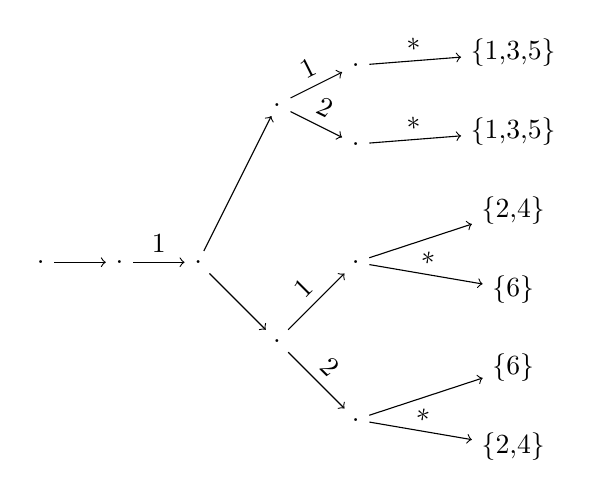
\begin{tikzpicture}[->,sloped,above]

		\node (root) at (0,2.5) {.};

		\node (h) at (1,2.5) {.};

		\node (h1) at (2,2.5) {.};

		\node (h1f) at (3,4.5) {.};
		\node (h1g) at (3,1.5) {.};

		\node (h1f1) at (4,5) {.};
		\node (h1f2) at (4,4) {.};
		\node (h1g1) at (4,2.5) {.};
		\node (h1g2) at (4,0.5) {.};

		\node (h1f1x) at (6,5) {\{1,3,5\}};
		\node (h1f2x) at (6,4) {\{1,3,5\}};
		\node (h1g1a) at (6,3) {\{2,4\}};
		\node (h1g1x) at (6,2) {\{6\}};
		\node (h1g2a) at (6,1) {\{6\}};
		\node (h1g2x) at (6,0) {\{2,4\}};

		\path
		(root) edge node {\( \mP \)} (h)

		(h) edge node {\( 1 \)} (h1)

		(h1)
		edge node {\( \mf \)} (h1f)
		edge node {\( \mg \)} (h1g)

		(h1f)
		edge node {\( 1 \)} (h1f1)
		edge node {\( 2 \)} (h1f2)

		(h1g)
		edge node {\( 1 \)} (h1g1)
		edge node {\( 2 \)} (h1g2)

		(h1f1)
		% edge node {\( \ma \)} (h1f1a)
		edge node {\( * \)} (h1f1x)

		(h1f2)
		%		edge node {\( \ma \)} (h1f2a)
		edge node {\( * \)} (h1f2x)


		(h1g1)
		edge node {\( \ma \)} (h1g1a)
		edge node {\( * \)} (h1g1x)

		(h1g2)
		edge node {\( \ma \)} (h1g2a)
		edge node {\( * \)} (h1g2x)

		;
		\end{tikzpicture}
	\end{center}
	%
	Now we retrieve candidate clauses with literals that clash with
	literal \( \lnot\mP(\mg(y',\mf(x'))) \):
%
\begin{gather*}
	\texttt{clashing}: \lnot\mP(\mg(y',\mf(x')))
	\mapsto \texttt{unifiable}: \{ \mP.1.\mg.1.{*}, \mP.1.\mg.2.\mf.1.* \}
	\mapsto \{ 2, 4, 6 \} \cap \{ 2, 4 \}
\end{gather*}
	\end{example}



\subsubsection{Redundant clauses}

In Resolution-based calculi
we can omit clauses that are subsumed
by other clauses, 
i.e.~weakened instances of clauses are redundant.
%
We will show in the following example and lemma 
that in contrast 
we must keep keep subsumed clauses
with \InstGen or \InstGenEQ.
We still can ommit some redundant clauses,
but the notion of redundancy is different from resolution.

\begin{example}\label{ex:not:equisat}
	The set of clauses \( S = \{ \,
	\mP(x), \lnot\mP(\mf(\ma))
	\, \} \) is clearly unsatisfiable, but
	\( S\bot \) is still satisfiable.
	We derive \( \mP(\mf(\ma)) \) which is subsumed by \( \mP(x) \),
	but can not ignore it because \( \{ \,
	\mP(\bot), \lnot\mP(\mf(\ma)), \mP(\mf(\ma))
	\, \} \) is unsatisfiable as desired.
\end{example}

\begin{lemma}
	If \( S = S' \cup \{ \mcD \} \),
	\( \mcC \in S' \), and there is a substitution \( \sigma \)
	such that \( \mcC\sigma \subseteq \mcD \)
	then
	\( S  \equisat S' \),
	but \( S\bot  \not\equisat S'\bot \).
\end{lemma}
\begin{proof}
	Obviously \( S'\cup \{ \mcD \} \entails S' \) and
	\( \mcC\sigma\entails\mcD \) by definition, hence
	\( S' \entails S'\cup \{ \mcD \} \) and
	\( S' \equiv S'\cup \{ \mcD \} \) which implies
	\( S' \equisat S' \cup \{ \mcD \} \).
%
	Although \( S'\bot\cup \{ \mcD\bot \} \entails S'\bot \)
	we have a counterexample to
	\( S'\bot \equisat S\bot \) with Example~\ref{ex:not:equisat},
	where \( C\sigma\bot \not\entails D\bot \),
	i.e.~\( \mP(\bot)\not\entails\mP(\mf(\ma)) \), but \( \mP(x)\entails\mP(\mf(\ma))  \).
\end{proof}
\begin{lemma}[Weakened variants]\label{lem:weakend:variants}
	If \( S = S' \cup \{ \mcD \} \),
	\( \mcC \in S' \), and there is a variable substitution \( \rho \)
	such that \( \mcC\rho \subseteq \mcD \)
	then
	\( S\bot\equisat S'\bot \).
\end{lemma}
\begin{proof}
	Since \( \rho \) is a variable substitution
	\( \mcC\rho\bot \entails \mcD\bot \) holds
	because \( \mcD\bot = \mcC\rho\bot \lor \mcD' \).
\end{proof}

\begin{example}
	\(
		\{ \ldots,
		\mP(x)\lor \mQ(y), \mP(z)\lor\mQ(z) \lor \mQ(\mf(z)) \}\bot
		\equisat
		\{ \ldots, \mP(x) \lor \mQ(y) \}\bot
	\)
	since \(
		(\mP(x)\lor\mQ(y)) \{x\mapsto z, y\mapsto z \}
		\subseteq
		\mP(z)\lor\mQ(z)\lor\mQ(\mf(z))
	\).
\end{example}

\begin{definition}[Backward removal]
	For a set of processed clauses \( P \)
	and a given (derived or unprocessed) clause \( \mcG \) we
	 remove clauses \( \mcD_i \) from \( P \) where
	 \( \mcG\rho_i \subseteq \mcD_i \) for some
	 variable substitution \( \rho_i \).
\end{definition}

\begin{definition}[Forward removal]
	For a set of processed clauses \( P \)
	we can omit a given (derived or unprocessed) clause \( \mcG \)
	if there exists a clause \( \mcC \in P \)
	and a variable substitution \( \rho \) such that \( \mcC\rho\subseteq \mcG \).
\end{definition}

	\begin{example}
		With variable agnostic term traversals we may encounter
		candidates for (weakened) variants that are actually not variants.
		There is no variable renaming \( \rho \) such that
		\( R(x,x,y) \rho = R(x',y',y') \) or
		\( R(x',y',y') \rho = R(x,x,y) \)
		but \( R.*.*.* \) matches perfectly.
	\end{example}

\subsubsection{Unifiable subterms}

For \InstGenEQ we have to quickly search for unifiable subterms of selected literals to apply unit superposition.

% PATH INDEXING/SubtermTrees
\begin{example} We have constructed the prefix tree for all subterms of the following literals. We annotate the references to our literals with the positions of the subterms (starting at the atom).
	\begin{gather*}
	\{
	\TI{1}\mP(\mh(\mf(x,x))),
	\TI{2}\lnot\mP(\mh(\mg(\ma,x))),
	\TI{3}\mP(\mh(\mf(y,z))),
	\\
	\TI{4}\lnot\mP(\mh(\mg(\ma,y))),
	\TI{5}\mP(\mh(\mf(y,x))),
	\TI{6}\lnot\mQ(\mh(\mg(y,a)),\ma)
	\}
	\end{gather*}
	%
	\begin{center}
		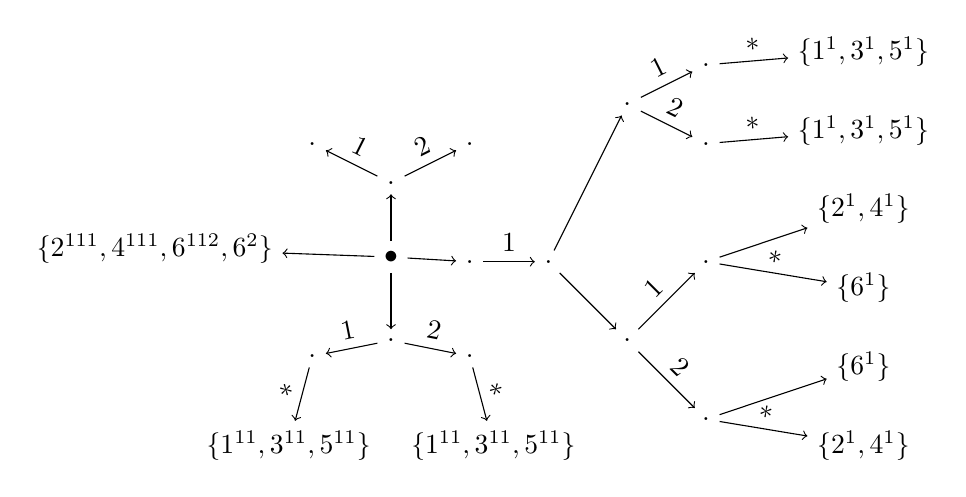
\begin{tikzpicture}[->,sloped,above]
		\node (root) at (0,2.5) {\( \bullet \)};
		%% right
		\node (h) at (1,2.5) {.};
		%
		\node (h1) at (2,2.5) {.};
		%
		\node (h1f) at (3,4.5) {.};
		\node (h1g) at (3,1.5) {.};
		%
		\node (h1f1) at (4,5) {.};
		\node (h1f2) at (4,4) {.};
		\node (h1g1) at (4,2.5) {.};
		\node (h1g2) at (4,0.5) {.};
		%
		\node (h1f1x) at (6,5) {\( \{1^1,3^1,5^1\} \)};
		\node (h1f2x) at (6,4) {\( \{1^1,3^1,5^1\} \)};
		\node (h1g1a) at (6,3) {\( \{2^1,4^1\} \)};
		\node (h1g1x) at (6,2) {\( \{6^1\} \)};
		\node (h1g2a) at (6,1) {\( \{6^1\} \)};
		\node (h1g2x) at (6,0) {\( \{2^1,4^1\} \)};
		%% down
		\node (f) at (0,1.5) {.};
		\node (f1) at (-1,1.3) {.};
		\node (f1x) at (-1.3,0) {\( \{1^{11},3^{11},5^{11}\} \)};
		\node (f2) at (1,1.3) {.};
		\node (f2x) at (1.3,0) {\( \{1^{11},3^{11},5^{11}\} \)};
		%% up
		\node (g) at (0,3.5) {.};
		\node (g1) at (-1,4) {.};
		\node (g2) at (1,4) {.};
		%% left
		\node (a) at (-3,2.5) {\( \{2^{111}, 4^{111}, 6^{112}, 6^2 \} \)};

		\path
		(root)
		edge node {\( \mh \)} (h)
		edge node {\( \mf \)} (f)
		edge node {\( \mg \)} (g)
		edge node {\( \ma \)} (a)

		(h) edge node {\( 1 \)} (h1)


		(h1)
		edge node {\( \mf \)} (h1f)
		edge node {\( \mg \)} (h1g)

		(h1f)
		edge node {\( 1 \)} (h1f1)
		edge node {\( 2 \)} (h1f2)

		(h1g)
		edge node {\( 1 \)} (h1g1)
		edge node {\( 2 \)} (h1g2)

		(h1f1)
		edge node {\( * \)} (h1f1x)

		(h1f2)
		edge node {\( * \)} (h1f2x)


		(h1g1)
		edge node {\( \ma \)} (h1g1a)
		edge node {\( * \)} (h1g1x)

		(h1g2)
		edge node {\( \ma \)} (h1g2a)
		edge node {\( * \)} (h1g2x)

		%
		(g) 	edge node {\( 1 \)} (g1)
		edge node {\( 2 \)} (g2)

		(f)	edge node {\( 1 \)} (f1)
		edge node {\( 2 \)} (f2)

		(f1)	edge node {\( * \)} (f1x)
		(f2)	edge node {\( * \)} (f2x)
		;


		\path (root)



		;

		\end{tikzpicture}
	\end{center}

	Now we retrieve literals with subterms that may be unifiable
	with terms \( \mf(\ma,\mb) \) and \( \mg(\ma,\mb) \).
	\begin{align*}
		\texttt{subterm}: \mf(\ma,\mb)
		&\mapsto \texttt{unifiable}: \{ \mf.1.\ma, \mf.2.\mb  \}
		\mapsto \{ 1^{11}, 3^{11}, 5^{11}  \}
		\\
		\texttt{subterm}: \mg(\ma,\mb)
		&\mapsto
		\texttt{unifiable}: \{ \mg.1.\ma, \mf.2.\ma  \}
		\mapsto
		\{ 2^{11}, 4^{11} \} \cap \{ 6^{11} \} = \emptyset
	\end{align*}
\end{example}

These outlined algorithms and data structures 
are just some of the theoretical building blocks for an actual prover. 
In the next chapter we discuss a practical implementation of a prover 
with these ideas and take a look how it performs on a wide variety of problems. 
















% % !TeX root = ../mythesis.tex
% !TeX encoding = UTF-8
% !TeX spellcheck = en_US

% \subsection{Motivation}
%% MOTIVATION %%

%- MOTIVATION/ClausalForm
%- MOTIVATION/Notation

%+ MOTIVATION/forwardSubsumption.tex

% \begin{example}[forward subsumption]
% 	\begin{gather*}
% 	S = \{ \TI{1}\mP(x,y), \TI{2}\lnot \mP(\ma,z)\} \cup \{\TI{3}\colG\mP(\ma,z') \}
% 	\tag*{\( \mcC_1 \) subsumes \( \mcC_3 \)}
% 	\\[0.7em]
% 	\infer[\{x\mapsto\ma,y\mapsto z\}]
% 	{\square}
% 	{\mP(x,y) & \lnot \mP(\ma,z)}
% 	\tag*{Resolution}
% 	\\[0.7em]
% 	S\bot = \{ \mP(\bot,\bot), {\colLo\lnot \mP(\ma,\bot), \mP(\ma,\bot)} \}
% 	\tag*{InstGen / SMT}
% 	\end{gather*}
% \end{example}

%+ MOTIVATION/goalEffectiveCalculus
%+ MOTIVATION/goalFastTermRetrieval
%+ MOTIVATION/goalSoundComplete


	% \begin{enumerate}
	% 	\item {Reduce} search space
	% 	\begin{itemize}
	% 		\item Ordered Resolution, Strategies, \ldots
	% 		\item \ldots with selection functions for clauses and literals
	% 	\end{itemize}
	% 	\item {Reduce} redundancy
	% 	\begin{itemize}
	% 		\item e.g.~discard clauses that are subsumed by other clauses
	% 		\item \ldots depending on the calculus
	% 	\end{itemize}
		% \item
		% Quickly find
		% \begin{itemize}
		% 	\item {variants} \hfill{\footnotesize variant removal}

		% 	\item {instances}   \hfill{\footnotesize backward subsumption}\\
		% 	\( \INST(s,t)\Leftrightarrow\exists\sigma\ s = t\sigma \)

		% 	\item {generalizations}  \hfill{\footnotesize forward subsumption}\\
		% 	\( \GNRL(s,t)\Leftrightarrow\exists\sigma\ s\sigma = t \)

		% 	\item {unifiable terms} \hfill{\footnotesize resolution, demodulation}\\
		% 	\( \UNIF(s,t)\Leftrightarrow\exists\sigma\ s\sigma = t\sigma \)

		% \end{itemize}

		% of a query term in a given set of terms.
	% \end{enumerate}




% \begin{tikzpicture}[scale = 1, transform shape, draw=black, fill=black, thick, sloped]

% \draw[->, ultra thick] (0,0) --
% node[pos=0, above] {\( F \)}
% (2,0);

% % outer rectangle
% \draw[rounded corners=-1.5mm] (1,3) rectangle (8.5,-3);
% % is F a theorem?
% \draw(2.4,2.7) node {\color{colN}Is \( F \) a theorem?};

% % SLIDE Is S satisfiable?
% \node[colG] (S) at (1.6,-2.7) {\scriptsize\( \lnot F \approx S \)};
% \node (S) at (2.5,0) {\( S \)};


% % SLIDE 2
% \draw[thin,dashed,draw=colO] (2.5,0) ellipse (0.4 and 1.2); % S

% % inner rectangle
% \draw[rounded corners=-1.5mm]  (1.5,-2.25) rectangle (8,2.25);
% % is S satisfiable?
% \draw (3.2,-1.9) node {\color{colN}Is \( \lnot F \) satisfiable?};

% % SLIDE unsatisfiable
% \draw[thin,dashed,draw=colO] (2.6,0) ellipse (0.6 and 1.44);  % S
% \draw[dashed, draw=colG, thick] decorate[decoration={snake}] {(1.4, 1) -- (8.2,0.6)};
% \draw[->, draw=colHi, ultra thick] (6.5,1.8) --
% node[pos=0,below] {unsatisfiable}
% node[pos=0.85, above] {theorem}
% (10,1.8) ;

% % SLIDE satisfiable
% \draw[thin,dashed,draw=colO] (2.8,0) ellipse (0.9 and 1.73);  % S
% \draw[dashed, draw=colG, thick]  decorate[decoration={snake}] { (1.4,-1)  --  (8.2,-0.6) };
% \draw[->,draw=colLo, ultra thick] (7,-1.3) --
% node[pos=0, below] {satisfiable}
% node[pos=0.75, above] {not a theorem} (11,-1.3) ;

% % SLIDE 5
% \draw[thin,dashed,draw=colO] (3.2,0) ellipse (1.35 and 2.07); % S
% \draw[->,draw=colNa, ultra thick] (7,0.15) --
% %	node[pos=0,above] {space out}
% node[pos=0,below] {time out}
% node[pos=0.85, above] {maybe} (10.5,0.15) ;
% \end{tikzpicture}

%%


%+ POSITION/Normalization
\begin{example}{Variable normalization}
	Variants of terms generate the same position strings
	\begin{itemize}
		\item if variable names are ignored
		\hfill \( \mf(y,z) \Rightarrow
		\ANGLES{\epsilon,\mf}
		\ANGLES{1,*}
		\ANGLES{2,*}
		 \)

		\item or normalized
		\hfill \( \mf(y,z) \Rightarrow
		\ANGLES{\epsilon,\mf}
		\ANGLES{1,x_1}
		\ANGLES{2,x_2} \)
		\\
		\hfill \( \mf(y,y) \Rightarrow
		\ANGLES{\epsilon,\mf}
		\ANGLES{1,x_1}
		\ANGLES{2,x_1}
		 \)
	\end{itemize}

	In the first case even non-variants of terms generate the same strings.
\end{example}


%+ POSITION/PositionStrings + Term traversals




%+ POSITION/Simplification


\subsection{Path Indexing}

%% PATH INDEXING %%

%+ PATH INDEXING/Build+Index
\begin{example}{Build}
	\def\TRIEWIDTH{4cm}
	\def\TEXTWIDTH{\textwidth-\TRIEWIDTH-2em}

	\begin{minipage}{\TEXTWIDTH}
		\(
		\TI{t_1}\,\mh(\mf(x,y)),
		\TI{t_2}\mh(\mf( x,\ma)),
		\TI{t_3}\mh(\mf(\ma,\ma))
		 \)
		\begin{align*}
		t_1 &\Rightarrow \{ \mh.1.\mf.1.{*},  \mh.1.\mf.2.{*} \} \\
		t_2 &\Rightarrow \{ \mh.1.\mf.1.{*},  \mh.1.\mf.2.\ma \} \\
		t_3 &\Rightarrow \{ \mh.1.\mf.1.\ma,  \mh.1.\mf.2 \ma \}
		\end{align*}
	\end{minipage}
%
	\begin{minipage}{\TRIEWIDTH}
	\begin{tikzpicture}[->,dotted]
%		\renewcommand{\PAUSE}{\pause}
%		\ORIGIN

\def\pyL{-0.2}
\def\pxL{0.05}

\PAUSE

\node (root) at (2.5,5) {.};
\node (h) at (2.5,4) {.};
\path (root) edge node {$\mh$} (h);

\PAUSE
\node (h1) at (2.5,3) {.};
\path (h) edge node {$1$} (h1);

\PAUSE
\node (h1f) at (1.5,2) {.};
\path (h1) edge node {$\mf$} (h1f);

\PAUSE
\node (h1f1) at (0.5,1) {.};
\path (h1f) edge node {$1$} (h1f1);

\PAUSE
\node (h1f1x) at (0,0) {.};
\path (h1f1) edge node {$*$} (h1f1x);
\node (12) at (\pxL,\pyL) {\scriptsize$t_1,t_2$};

\PAUSE
\node (h1f1a) at (1,0) {.};
\path (h1f1) edge node {$\ma$} (h1f1a);
\node (3) at (\pxL+1,\pyL) {\scriptsize$t_3$};

\PAUSE
\node (h1f2) at (2.5,1) {.};
\path (h1f) edge node {$2$} (h1f2);

\PAUSE
\node (h1f2x) at (2,0) {.};
\path (h1f2) edge node {$*$} (h1f2x);
\node (1) at (\pxL+2,\pyL) {\scriptsize$t_1$};

\PAUSE
\node (h1f2a) at (3,0) {.};
\path (h1f2) edge node {$\ma$} (h1f2a);
\node (23) at (\pxL+3,\pyL) {\scriptsize$t_2,t_3$};


\node (lu) at (0,-0.5) {} ;
\ORIGIN

\def\pyL{-0.2}
\def\pxL{0.05}

\node (root) at (2.5,5) {.};
\node (h) at (2.5,4) {.};
\path (root) edge node {$\mh$} (h);

\node (h1) at (2.5,3) {.};
\path (h) edge node {$1$} (h1);

\node (h1f) at (1.5,2) {.};
\path (h1) edge node {$\mf$} (h1f);

\node (h1f1) at (0.5,1) {.};
\path (h1f) edge node {$1$} (h1f1);

\node (h1f1x) at (0,0) {.};
\path (h1f1) edge node {$*$} (h1f1x);
\node (12) at (\pxL,\pyL) {\scriptsize$t_1,t_2$};

\node (h1f1a) at (1,0) {.};
\path (h1f1) edge node {$\ma$} (h1f1a);
\node (3) at (\pxL+1,\pyL) {\scriptsize$t_3$};

\node (h1f2) at (2.5,1) {.};
\path (h1f) edge node {$2$} (h1f2);

\node (h1f2x) at (2,0) {.};
\path (h1f2) edge node {$*$} (h1f2x);
\node (1) at (\pxL+2,\pyL) {\scriptsize$t_1$};

\node (h1f2a) at (3,0) {.};
\path (h1f2) edge node {$\ma$} (h1f2a);
\node (23) at (\pxL+3,\pyL) {\scriptsize$t_2,t_3$};

\node (lu) at (0,-0.5) {} ;

		\end{tikzpicture}
	\end{minipage}
\end{example}


%+ PATH INDEXING/PathStrings
\begin{example}{Path strings}
	The path-strings of \( \mh(\mf(\ma,y)) \) are
	{\( \mh. 1. \mf. 1. \ma \)} and
	{\( \mh. 1. \mf. 2. {*} \)}.

	\begin{tikzpicture}[->,right]
	\node (root) at (0.1,0) {};
	\node (h) at (0,-1) {\( \mh \)};
	\node (hf) at (0,-2) {\( \mf \)};
	\node (hfa) at (-1,-3) {\( \ma \)};
	\node (hfy) at (1,-3) {\( y \)};
	\node (bottom) at (1,-4) {};

	\path (root) edge node{\( \varepsilon \)} (h)
	(h) edge node {1} (hf)
	(hf)
	edge node[above,sloped] {1} (hfa)
	edge node[above,sloped] {2} (hfy)
	;
	\end{tikzpicture}
	\hspace{2em}
	%
	\def\dx{1.5}
	\def\wx{2.0}
	%
	\begin{tikzpicture}[->,right]

	\node (0) at (0,1.4) {.};
	\node (root) at (0,0.7) {.};
	\node (h) at (0,0) {.};
	\node (h1) at (0,-.7) {.};
	\node (h1f) at (0,-1.4) {.};
	\node (h1f1) at (0,-2.1) {.};
	\node (h1f1a) at (0,-2.8) {.};

	\path (0) edge node {\( \varepsilon \)} (root)
	(root) edge node {\( \mh \)} (h)
	(h) edge node {\( 1 \)} (h1)
	(h1) edge node {\( \mf \)} (h1f)
	(h1f) edge node {\( 1 \)} (h1f1)
	(h1f1) edge node {\( \ma \)} (h1f1a);


	\node (0) at (\dx,1.4) {.};
	\node (root) at (\dx,0.7) {.};
	\node (h) at (\dx,0) {.};
	\node (h1) at (\dx,-.7) {.};
	\node (h1f) at (\dx,-1.4) {.};
	\node (h1f1) at (\dx,-2.1) {.};
	\node (h1f1a) at (\dx,-2.8) {.};

	\path (0) edge node {\( \varepsilon \)} (root)
	(root) edge node {\( \mh \)} (h)
	(h) edge node {\( 1 \)} (h1)
	(h1) edge node {\( \mf \)} (h1f)
	(h1f) edge node {\( 2 \)} (h1f1)
	(h1f1) edge node {\( * \)} (h1f1a);

	\node (0) at (2*\dx+\wx/2,1.4) {.};
	\node (root) at (2*\dx+\wx/2,0.7) {.};
	\node (h) at (2*\dx+\wx/2,0) {.};
	\node (h1) at (2*\dx+\wx/2,-.7) {.};
	\node (h1f) at (2*\dx+\wx/2,-1.4) {.};
	\node (h1f1) at (2*\dx,-2.1) {.};
	\node (h1f1a) at (2*\dx,-3) {.};
	\node (h1f2) at (2*\dx+\wx,-2.1) {.};
	\node (h1f2x) at (2*\dx+\wx,-3) {.};

	\path (0) edge node {\( \varepsilon \)} (root)
	(root) edge node {\( \mh \)} (h)
	(h) edge node {\( 1 \)} (h1)
	(h1) edge node {\( \mf \)} (h1f)
	(h1f) edge node[above,sloped] {\( 1 \)} (h1f1)
	(h1f1) edge node {\( \ma \)} (h1f1a)
	(h1f) edge node[above,sloped] {\( 2 \)} (h1f2)
	(h1f2) edge node {\( * \)} (h1f2x);


	\end{tikzpicture}
\end{example}

% PATH INDEXING/PrefixTrees
\begin{example}[Prefix Trees]
\begin{gather*}
\{
\TI{1}\mh(\mf(x,x)),
\TI{2}\mh(\mg(\ma,x)),
\TI{3}\mh(\mf(y,z))
\TI{4}\mh(\mg(\ma,y)),
\TI{5}\mh(\mf(y,x)),
\TI{6}\mh(\mg(y,a))
\}
\end{gather*}
%
\begin{center}
	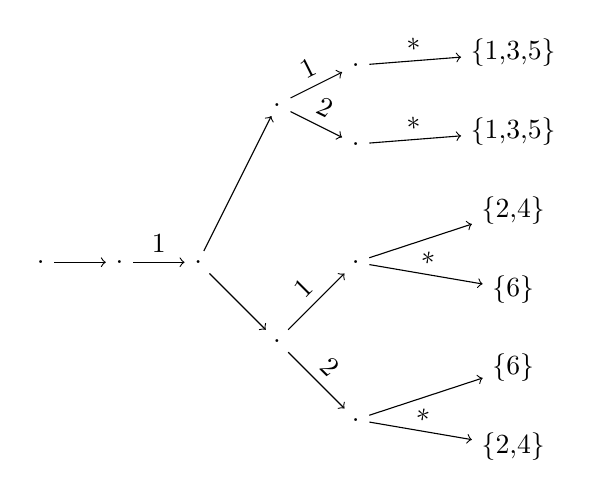
\begin{tikzpicture}[->,sloped,above]

	\node (root) at (0,2.5) {.};

	\node (h) at (1,2.5) {.};

	\node (h1) at (2,2.5) {.};

	\node (h1f) at (3,4.5) {.};
	\node (h1g) at (3,1.5) {.};

	\node (h1f1) at (4,5) {.};
	\node (h1f2) at (4,4) {.};
	\node (h1g1) at (4,2.5) {.};
	\node (h1g2) at (4,0.5) {.};

	\node (h1f1x) at (6,5) {\{1,3,5\}};
	\node (h1f2x) at (6,4) {\{1,3,5\}};
	\node (h1g1a) at (6,3) {\{2,4\}};
	\node (h1g1x) at (6,2) {\{6\}};
	\node (h1g2a) at (6,1) {\{6\}};
	\node (h1g2x) at (6,0) {\{2,4\}};

	\path (root) edge node {\( \mh \)} (h)
	(h) edge node {\( 1 \)} (h1)

	(h1)
	edge node {\( \mf \)} (h1f)
	edge node {\( \mg \)} (h1g)

	(h1f)
	edge node {\( 1 \)} (h1f1)
	edge node {\( 2 \)} (h1f2)

	(h1g)
	edge node {\( 1 \)} (h1g1)
	edge node {\( 2 \)} (h1g2)

	(h1f1)
	% edge node {\( \ma \)} (h1f1a)
	edge node {\( * \)} (h1f1x)

	(h1f2)
	%		edge node {\( \ma \)} (h1f2a)
	edge node {\( * \)} (h1f2x)


	(h1g1)
	edge node {\( \ma \)} (h1g1a)
	edge node {\( * \)} (h1g1x)

	(h1g2)
	edge node {\( \ma \)} (h1g2a)
	edge node {\( * \)} (h1g2x)
	;
	\end{tikzpicture}
\end{center}
\( \mh(\mg(y,x)) \mapsto \{ \mh.1.\mg.1.{*}, \mh.1.\mg.2.{*} \} \)
\end{example}

%+ PATH INDEXING/Retrieve
\begin{example}{Retrieve}
	\def\TRIEWIDTH{5cm}
	\def\TEXTWIDTH{\textwidth-\TRIEWIDTH-2em}

	\begin{minipage}{\TEXTWIDTH}
		\(
		\TI{t_1}\mh(\mf(x,y)),
		\TI{t_2}\mh(\mf({ x},{\ma})),
		\TI{t_3}\mh(\mf(\ma,\ma))
		 \)
		\begin{align*}
		\mh(\mf(z,\mb)) &\Rightarrow \{ \mh.1.\mf.1.{*}, \mh.1.\mf.2.\mb \}
		\\[0.7em]
		u : \mh(\mf({\colN z},{\colHi \mb}))
		& \mapsto
		{
			\{ t_1, {\colG t_2},
			{t_3} \}
		}
		{
			\cap \{t_1 \}
		}\\
%		{
			i : \mh(\mf(z, \mb)) &\mapsto \{ {\colG t_1,t_2,t_3 } \} \cap \{  \}
%		}
	\\
%		{
			g : \mh(\mf(z, \mb)) &\mapsto \{ t_1, {\colG t_2} \} \cap \{ t_1 \}
%		}
	\\
%		{
			v : \mh(\mf(z, \mb)) &\mapsto \{ {\colG t_1,t_2 }\} \cap \{  \}
%		}
	\\[0.7em]
%		{
			\colG v: \mh(\mf(z, z)) &\mapsto \{ {\colLo t_1},{\colG t_2} \} \cap \{ {\colLo t_1} \}
%		}
	\end{align*}
	\end{minipage}
	%
	\begin{minipage}{{\TRIEWIDTH}}
		\begin{tikzpicture}[->,dotted]
%		\ORIGIN

\def\pyL{-0.2}
\def\pxL{0.05}

\PAUSE

\node (root) at (2.5,5) {.};
\node (h) at (2.5,4) {.};
\path (root) edge node {$\mh$} (h);

\PAUSE
\node (h1) at (2.5,3) {.};
\path (h) edge node {$1$} (h1);

\PAUSE
\node (h1f) at (1.5,2) {.};
\path (h1) edge node {$\mf$} (h1f);

\PAUSE
\node (h1f1) at (0.5,1) {.};
\path (h1f) edge node {$1$} (h1f1);

\PAUSE
\node (h1f1x) at (0,0) {.};
\path (h1f1) edge node {$*$} (h1f1x);
\node (12) at (\pxL,\pyL) {\scriptsize$t_1,t_2$};

\PAUSE
\node (h1f1a) at (1,0) {.};
\path (h1f1) edge node {$\ma$} (h1f1a);
\node (3) at (\pxL+1,\pyL) {\scriptsize$t_3$};

\PAUSE
\node (h1f2) at (2.5,1) {.};
\path (h1f) edge node {$2$} (h1f2);

\PAUSE
\node (h1f2x) at (2,0) {.};
\path (h1f2) edge node {$*$} (h1f2x);
\node (1) at (\pxL+2,\pyL) {\scriptsize$t_1$};

\PAUSE
\node (h1f2a) at (3,0) {.};
\path (h1f2) edge node {$\ma$} (h1f2a);
\node (23) at (\pxL+3,\pyL) {\scriptsize$t_2,t_3$};


\node (lu) at (0,-0.5) {} ;
		\ORIGIN

\def\pyL{-0.2}
\def\pxL{0.05}

\node (root) at (2.5,5) {.};
\node (h) at (2.5,4) {.};
\path (root) edge node {$\mh$} (h);

\node (h1) at (2.5,3) {.};
\path (h) edge node {$1$} (h1);

\node (h1f) at (1.5,2) {.};
\path (h1) edge node {$\mf$} (h1f);

\node (h1f1) at (0.5,1) {.};
\path (h1f) edge node {$1$} (h1f1);

\node (h1f1x) at (0,0) {.};
\path (h1f1) edge node {$*$} (h1f1x);
\node (12) at (\pxL,\pyL) {\scriptsize$t_1,t_2$};

\node (h1f1a) at (1,0) {.};
\path (h1f1) edge node {$\ma$} (h1f1a);
\node (3) at (\pxL+1,\pyL) {\scriptsize$t_3$};

\node (h1f2) at (2.5,1) {.};
\path (h1f) edge node {$2$} (h1f2);

\node (h1f2x) at (2,0) {.};
\path (h1f2) edge node {$*$} (h1f2x);
\node (1) at (\pxL+2,\pyL) {\scriptsize$t_1$};

\node (h1f2a) at (3,0) {.};
\path (h1f2) edge node {$\ma$} (h1f2a);
\node (23) at (\pxL+3,\pyL) {\scriptsize$t_2,t_3$};

\node (lu) at (0,-0.5) {} ;

		\path[bend right, dashed, colN](root) edge (h);
		\node at (1.3,5) {\scriptsize\( (\mh,1.\mf.1.{*}) \)};
		\path[bend right, dashed, colN]	(h) edge (h1);
		\node at (1.0,4) {\scriptsize\( (1,\mf.1.{*}) \)};
		\path[bend right, dashed, colN]	(h1) edge (h1f);
		\node at (0.7,3) {\scriptsize\( (\mf,1.{*}) \)};
		\path[bend right, dashed, colN]	(h1f) edge (h1f1);
		\node at (0.4,2) {\scriptsize\( (1,{*}) \)};
		\path[bend right, dashed, colN]	(h1f1) edge (h1f1x)	;
		\node at (0.1,1) {\scriptsize\( ({*},\epsilon) \)};
		\path[bend right, dashed, colN]	(h1f1) edge (h1f1a);

		\path[bend left, dashed, colHi]	(root) edge (h)	;
		\node at (3.5,5) {\scriptsize\( (\mh,1.\mf.2.\mb) \)};
		\path[bend left, dashed, colHi]	(h) edge (h1)	;
		\node at (3.4,4) {\scriptsize\( (1,\mf.2.\mb) \)};
		\path[bend left, dashed, colHi]	(h1) edge (h1f)	;
		\node at (3.3,3) {\scriptsize\( (\mf,2.\mb) \)};
		\path[bend left, dashed, colHi]	(h1f) edge (h1f2)	;
		\node at (3.2,2) {\scriptsize\( (2,\mb) \)};
		\path[bend left, dashed, colHi]	(h1f2) edge (h1f2x)	;
		\node at (3.1,1) {\scriptsize\( (\mb,\epsilon) \)};
		\end{tikzpicture}
	\end{minipage}
\end{example}

%+ PATH INDEXING/Subterms
\begin{example}{Demodulation (Subterms)}

	\(
	\colG
	\TI{t_1}\mh(\mf(x,y)),
	\TI{t_2}\mh(\mf({ x},{\ma})),
	\TI{t_3}\mh(\mf(\ma,\ma)),
	\ldots,
%	\color{black}\mf(x,\ma) \foEQ x
	\color{black}\mf(x,\ma) \mEQ x
	 \)


	 \def\TRIEWIDTH{\textwidth/2-1em}% chktex 8
	 \def\TEXTWIDTH{\textwidth-\TRIEWIDTH-2em}
	\begin{minipage}{\TEXTWIDTH}
		\begin{tikzpicture}[->,dotted]
%		\ORIGIN

\def\pyL{-0.2}
\def\pxL{0.05}

\PAUSE

\node (root) at (2.5,5) {.};
\node (h) at (2.5,4) {.};
\path (root) edge node {$\mh$} (h);

\PAUSE
\node (h1) at (2.5,3) {.};
\path (h) edge node {$1$} (h1);

\PAUSE
\node (h1f) at (1.5,2) {.};
\path (h1) edge node {$\mf$} (h1f);

\PAUSE
\node (h1f1) at (0.5,1) {.};
\path (h1f) edge node {$1$} (h1f1);

\PAUSE
\node (h1f1x) at (0,0) {.};
\path (h1f1) edge node {$*$} (h1f1x);
\node (12) at (\pxL,\pyL) {\scriptsize$t_1,t_2$};

\PAUSE
\node (h1f1a) at (1,0) {.};
\path (h1f1) edge node {$\ma$} (h1f1a);
\node (3) at (\pxL+1,\pyL) {\scriptsize$t_3$};

\PAUSE
\node (h1f2) at (2.5,1) {.};
\path (h1f) edge node {$2$} (h1f2);

\PAUSE
\node (h1f2x) at (2,0) {.};
\path (h1f2) edge node {$*$} (h1f2x);
\node (1) at (\pxL+2,\pyL) {\scriptsize$t_1$};

\PAUSE
\node (h1f2a) at (3,0) {.};
\path (h1f2) edge node {$\ma$} (h1f2a);
\node (23) at (\pxL+3,\pyL) {\scriptsize$t_2,t_3$};


\node (lu) at (0,-0.5) {} ;
		\ORIGIN

\def\pyL{-0.2}
\def\pxL{0.05}

\node (root) at (2.5,5) {.};
\node (h) at (2.5,4) {.};
\path (root) edge node {$\mh$} (h);

\node (h1) at (2.5,3) {.};
\path (h) edge node {$1$} (h1);

\node (h1f) at (1.5,2) {.};
\path (h1) edge node {$\mf$} (h1f);

\node (h1f1) at (0.5,1) {.};
\path (h1f) edge node {$1$} (h1f1);

\node (h1f1x) at (0,0) {.};
\path (h1f1) edge node {$*$} (h1f1x);
\node (12) at (\pxL,\pyL) {\scriptsize$t_1,t_2$};

\node (h1f1a) at (1,0) {.};
\path (h1f1) edge node {$\ma$} (h1f1a);
\node (3) at (\pxL+1,\pyL) {\scriptsize$t_3$};

\node (h1f2) at (2.5,1) {.};
\path (h1f) edge node {$2$} (h1f2);

\node (h1f2x) at (2,0) {.};
\path (h1f2) edge node {$*$} (h1f2x);
\node (1) at (\pxL+2,\pyL) {\scriptsize$t_1$};

\node (h1f2a) at (3,0) {.};
\path (h1f2) edge node {$\ma$} (h1f2a);
\node (23) at (\pxL+3,\pyL) {\scriptsize$t_2,t_3$};

\node (lu) at (0,-0.5) {} ;

		\node (f) at (1.5,4) {.};
		\path[colN] (root) edge node {f} (f);

		\node (f1) at (0.5,4) {.};
		\path[colN] (f) edge node {1} (f1);

		\node (f1x) at (-0.5,4) {};
		\path[colN] (f1)	edge node {*} (f1x);

		\node[colN] (t1) at (-0.5,4.2) {\scriptsize\( t_1^1 \)};
		\node[colN] (t1) at (-0.5,3.8) {\scriptsize\(  t_2^1 \)};

		\node (f1a) at (-0.5,3) {};
		\path[colN] (f1) edge node {a} (f1a);

		\node[colN] (t3) at (-0.5,2.9) {\scriptsize\( t_3^1 \)};

		\node (f2) at (0.5,3) {.};
		\path[colN] (f) edge node {2}  (f2);

		\node (f2x) at (-0.5,2) {};
		\path[colN] (f2) edge node {*} (f2x);

		\node[colN] (t1) at (-0.5,1.9) {\scriptsize\( t_1^1 \)};

		\node (f2a) at (0.5,2) {};
		\path[colN] (f2) edge node {a} (f2a);

		\node[colN] (t2t3) at (0.5,1.9) {\scriptsize\( t_2^1,t_3^1 \)};

		\node (a) at (3.5,4) {};
		\path[colN] (root)  edge node {\( \ma \)} (a);
		\node[colN] (t2t3t3) at (3.5,3.9) {\scriptsize\( t_2^{12},t_3^{11,12} \)};

		\end{tikzpicture}
	\end{minipage}
	\hfill
	\begin{minipage}{{\TRIEWIDTH}}
		\def\pyL{-0.2}
		\def\pxL{0.05}
		\begin{tikzpicture}[->,dotted]
%		\ORIGIN

\def\pyL{-0.2}
\def\pxL{0.05}

\PAUSE

\node (root) at (2.5,5) {.};
\node (h) at (2.5,4) {.};
\path (root) edge node {$\mh$} (h);

\PAUSE
\node (h1) at (2.5,3) {.};
\path (h) edge node {$1$} (h1);

\PAUSE
\node (h1f) at (1.5,2) {.};
\path (h1) edge node {$\mf$} (h1f);

\PAUSE
\node (h1f1) at (0.5,1) {.};
\path (h1f) edge node {$1$} (h1f1);

\PAUSE
\node (h1f1x) at (0,0) {.};
\path (h1f1) edge node {$*$} (h1f1x);
\node (12) at (\pxL,\pyL) {\scriptsize$t_1,t_2$};

\PAUSE
\node (h1f1a) at (1,0) {.};
\path (h1f1) edge node {$\ma$} (h1f1a);
\node (3) at (\pxL+1,\pyL) {\scriptsize$t_3$};

\PAUSE
\node (h1f2) at (2.5,1) {.};
\path (h1f) edge node {$2$} (h1f2);

\PAUSE
\node (h1f2x) at (2,0) {.};
\path (h1f2) edge node {$*$} (h1f2x);
\node (1) at (\pxL+2,\pyL) {\scriptsize$t_1$};

\PAUSE
\node (h1f2a) at (3,0) {.};
\path (h1f2) edge node {$\ma$} (h1f2a);
\node (23) at (\pxL+3,\pyL) {\scriptsize$t_2,t_3$};


\node (lu) at (0,-0.5) {} ;
		\ORIGIN

\def\pyL{-0.2}
\def\pxL{0.05}

\node (root) at (2.5,5) {.};
\node (h) at (2.5,4) {.};
\path (root) edge node {$\mh$} (h);

\node (h1) at (2.5,3) {.};
\path (h) edge node {$1$} (h1);

\node (h1f) at (1.5,2) {.};
\path (h1) edge node {$\mf$} (h1f);

\node (h1f1) at (0.5,1) {.};
\path (h1f) edge node {$1$} (h1f1);

\node (h1f1x) at (0,0) {.};
\path (h1f1) edge node {$*$} (h1f1x);
\node (12) at (\pxL,\pyL) {\scriptsize$t_1,t_2$};

\node (h1f1a) at (1,0) {.};
\path (h1f1) edge node {$\ma$} (h1f1a);
\node (3) at (\pxL+1,\pyL) {\scriptsize$t_3$};

\node (h1f2) at (2.5,1) {.};
\path (h1f) edge node {$2$} (h1f2);

\node (h1f2x) at (2,0) {.};
\path (h1f2) edge node {$*$} (h1f2x);
\node (1) at (\pxL+2,\pyL) {\scriptsize$t_1$};

\node (h1f2a) at (3,0) {.};
\path (h1f2) edge node {$\ma$} (h1f2a);
\node (23) at (\pxL+3,\pyL) {\scriptsize$t_2,t_3$};

\node (lu) at (0,-0.5) {} ;

		\node[colN] (n-hsubs) at (5,4) {\( \mh \)};
		\path[dashdotted, above, pos=0.3,sloped,bend right=5,colN]  (n-hsubs) edge node {\scriptsize\( \ANGLES{\epsilon,\mh} \)} (h);

		\node[colN] (n-fsubs) at (5,3) {\( \mf \)};
		\path[dashdotted, above, pos=0.3,sloped, bend right=10,colN]  (n-fsubs) edge node {\scriptsize\( \ANGLES{1,\mf} \)} (h1f);

		\node[colN] (n-asubs) at (5,2) {\( \ma \)};
		\path[dashdotted, above, bend right, pos=0.3,sloped,colN]  (n-asubs) edge node {\scriptsize\( \ANGLES{11,\ma} \)} (h1f1a);
		\path[dashdotted, bend right, below, pos=0.3,sloped,colN]  (n-asubs) edge node {\scriptsize\( \ANGLES{12,\ma} \)} (h1f2a);

		\end{tikzpicture}
	\end{minipage}


\end{example}

%+ PATH INDEXING/SubtermTrees
\begin{example}{Subterm trees}
\begin{gather*}
\{
\TI{1}\mh(\mf(x,x)),
\TI{2}\mh(\mg(\ma,x)),
\TI{3}\mh(\mf(y,z))
\TI{4}\mh(\mg(\ma,y)),
\TI{5}\mh(\mf(y,x)),
\TI{6}\mh(\mg(y,a))
\}
\end{gather*}
%
\begin{center}
	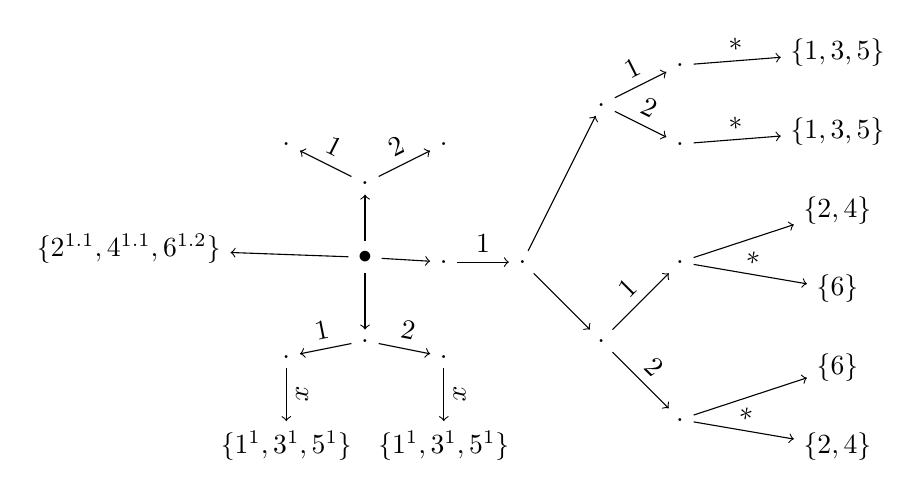
\begin{tikzpicture}[->,sloped,above]
	\node (root) at (0,2.5) {\( \bullet \)};
	%% right
	\node (h) at (1,2.5) {.};
	%
	\node (h1) at (2,2.5) {.};
	%
	\node (h1f) at (3,4.5) {.};
	\node (h1g) at (3,1.5) {.};
	%
	\node (h1f1) at (4,5) {.};
	\node (h1f2) at (4,4) {.};
	\node (h1g1) at (4,2.5) {.};
	\node (h1g2) at (4,0.5) {.};
	%
	\node (h1f1x) at (6,5) {\( \{1,3,5\} \)};
	\node (h1f2x) at (6,4) {\( \{1,3,5\} \)};
	\node (h1g1a) at (6,3) {\( \{2,4\} \)};
	\node (h1g1x) at (6,2) {\( \{6\} \)};
	\node (h1g2a) at (6,1) {\( \{6\} \)};
	\node (h1g2x) at (6,0) {\( \{2,4\} \)};
	%% down
	\node (f) at (0,1.5) {.};
	\node (f1) at (-1,1.3) {.};
	\node (f1x) at (-1,0) {\( \{1^{1},3^{1},5^{1}\} \)};
	\node (f2) at (1,1.3) {.};
	\node (f2x) at (1,0) {\( \{1^{1},3^{1},5^{1}\} \)};
	%% up
	\node (g) at (0,3.5) {.};
	\node (g1) at (-1,4) {.};
	\node (g2) at (1,4) {.};
	%% left
	\node (a) at (-3,2.5) {\( \{2^{1.1}, 4^{1.1}, 6^{1.2}\} \)};

	\path
	(root)
	edge node {\( \mh \)} (h)
	edge node {\( \mf \)} (f)
	edge node {\( \mg \)} (g)
	edge node {\( \ma \)} (a)

	(h) edge node {\( 1 \)} (h1)


	(h1)
	edge node {\( \mf \)} (h1f)
	edge node {\( \mg \)} (h1g)

	(h1f)
	edge node {\( 1 \)} (h1f1)
	edge node {\( 2 \)} (h1f2)

	(h1g)
	edge node {\( 1 \)} (h1g1)
	edge node {\( 2 \)} (h1g2)

	(h1f1)
	edge node {\( * \)} (h1f1x)

	(h1f2)
	edge node {\( * \)} (h1f2x)


	(h1g1)
	edge node {\( \ma \)} (h1g1a)
	edge node {\( * \)} (h1g1x)

	(h1g2)
	edge node {\( \ma \)} (h1g2a)
	edge node {\( * \)} (h1g2x)

	%
	(g) 	edge node {\( 1 \)} (g1)
	edge node {\( 2 \)} (g2)

	(f)	edge node {\( 1 \)} (f1)
	edge node {\( 2 \)} (f2)

	(f1)	edge node {\( x \)} (f1x)
	(f2)	edge node {\( x \)} (f2x)
	;


	\path (root)



	;

	\end{tikzpicture}
\end{center}
\end{example}





\subsection{Substitution Tree}
%% SUBSTITUTION TREES

%+ SUBSTITUTION TREES/Build+Index
\begin{example}{Substitution tree build}

	\(
	\TI{t_1}\mh(\mf(x,y)),
	\TI{t_2}\mh(\mf(x,\mh(\ma))),
	\TI{t_3}\mh(\mf(\mh(\ma),\ma)),
	\TI{t_4}\mh(\mf(\ma,\ma))
	 \)

	\begin{tikzpicture}[->]
%	\ORIGIN

\def\pyL{-0.2}
\def\pxL{0.05}

\PAUSE

\node (root) at (2.5,5) {.};
\node (h) at (2.5,4) {.};
\path (root) edge node {$\mh$} (h);

\PAUSE
\node (h1) at (2.5,3) {.};
\path (h) edge node {$1$} (h1);

\PAUSE
\node (h1f) at (1.5,2) {.};
\path (h1) edge node {$\mf$} (h1f);

\PAUSE
\node (h1f1) at (0.5,1) {.};
\path (h1f) edge node {$1$} (h1f1);

\PAUSE
\node (h1f1x) at (0,0) {.};
\path (h1f1) edge node {$*$} (h1f1x);
\node (12) at (\pxL,\pyL) {\scriptsize$t_1,t_2$};

\PAUSE
\node (h1f1a) at (1,0) {.};
\path (h1f1) edge node {$\ma$} (h1f1a);
\node (3) at (\pxL+1,\pyL) {\scriptsize$t_3$};

\PAUSE
\node (h1f2) at (2.5,1) {.};
\path (h1f) edge node {$2$} (h1f2);

\PAUSE
\node (h1f2x) at (2,0) {.};
\path (h1f2) edge node {$*$} (h1f2x);
\node (1) at (\pxL+2,\pyL) {\scriptsize$t_1$};

\PAUSE
\node (h1f2a) at (3,0) {.};
\path (h1f2) edge node {$\ma$} (h1f2a);
\node (23) at (\pxL+3,\pyL) {\scriptsize$t_2,t_3$};


\node (lu) at (0,-0.5) {} ;
	\ORIGIN


\node (root) at (0,0) {.};
\node (h) at (0,-1) {\( *_0 \mapsto \mh(*_1) \)};
\path (root) edge (h);

\node (f) at (0,-2) {\( *_1 \mapsto \mf(*_2,*_3) \)};
\path (h) edge (f);

\node (x2x) at (-2,-3) {\( *_2 \mapsto x \)} ;
\path (f) edge (x2x);

\node (x3y) at (-3,-4) {\( *_3 \mapsto y \)};
\path (x2x) edge (x3y);
\node (t1) at (-3,-4.4) {\( t_1 \)};

\node (x3ha) at (-1,-4) {\( *_3 \mapsto \mh(\ma) \)};
\path (x2x) edge (x3ha);
\node (t2) at (-1,-4.4) {\( t_2 \)};

\node (x3a)at (2,-3) {\( *_3\mapsto\ma \)};
\path (f) edge (x3a);

\node (x2ha) at (1,-4) {\( *_2\mapsto\mh(\ma) \)};
\path (x3a) edge (x2ha);
\node (t3) at (1,-4.4) {\( t_3 \)};

\node (x2a) at (3,-4) {\( *_2\mapsto\ma \)};
\path (x3a) edge (x2a);
\node (t4) at (3,-4.4) {\( t_4 \)};

	\end{tikzpicture}
\end{example}

%+ SUBSTITUTION TREES/Retrieve+Index
\begin{example}{Substitution tree retrieve}

	\(
	\TI{t_1}\mh(\mf(x,y)),
	\TI{t_2}\mh(\mf(x,\mh(\ma))),
	\TI{t_3}\mh(\mf(\mh(\ma),\ma)),
	\TI{t_4}\mh(\mf(\ma,\ma))
	 \)

	\begin{tikzpicture}[->]
%	\ORIGIN

\def\pyL{-0.2}
\def\pxL{0.05}

\PAUSE

\node (root) at (2.5,5) {.};
\node (h) at (2.5,4) {.};
\path (root) edge node {$\mh$} (h);

\PAUSE
\node (h1) at (2.5,3) {.};
\path (h) edge node {$1$} (h1);

\PAUSE
\node (h1f) at (1.5,2) {.};
\path (h1) edge node {$\mf$} (h1f);

\PAUSE
\node (h1f1) at (0.5,1) {.};
\path (h1f) edge node {$1$} (h1f1);

\PAUSE
\node (h1f1x) at (0,0) {.};
\path (h1f1) edge node {$*$} (h1f1x);
\node (12) at (\pxL,\pyL) {\scriptsize$t_1,t_2$};

\PAUSE
\node (h1f1a) at (1,0) {.};
\path (h1f1) edge node {$\ma$} (h1f1a);
\node (3) at (\pxL+1,\pyL) {\scriptsize$t_3$};

\PAUSE
\node (h1f2) at (2.5,1) {.};
\path (h1f) edge node {$2$} (h1f2);

\PAUSE
\node (h1f2x) at (2,0) {.};
\path (h1f2) edge node {$*$} (h1f2x);
\node (1) at (\pxL+2,\pyL) {\scriptsize$t_1$};

\PAUSE
\node (h1f2a) at (3,0) {.};
\path (h1f2) edge node {$\ma$} (h1f2a);
\node (23) at (\pxL+3,\pyL) {\scriptsize$t_2,t_3$};


\node (lu) at (0,-0.5) {} ;
	\ORIGIN


\node (root) at (0,0) {.};
\node (h) at (0,-1) {\( *_0 \mapsto \mh(*_1) \)};
\path (root) edge (h);

\node (f) at (0,-2) {\( *_1 \mapsto \mf(*_2,*_3) \)};
\path (h) edge (f);

\node (x2x) at (-2,-3) {\( *_2 \mapsto x \)} ;
\path (f) edge (x2x);

\node (x3y) at (-3,-4) {\( *_3 \mapsto y \)};
\path (x2x) edge (x3y);
\node (t1) at (-3,-4.4) {\( t_1 \)};

\node (x3ha) at (-1,-4) {\( *_3 \mapsto \mh(\ma) \)};
\path (x2x) edge (x3ha);
\node (t2) at (-1,-4.4) {\( t_2 \)};

\node (x3a)at (2,-3) {\( *_3\mapsto\ma \)};
\path (f) edge (x3a);

\node (x2ha) at (1,-4) {\( *_2\mapsto\mh(\ma) \)};
\path (x3a) edge (x2ha);
\node (t3) at (1,-4.4) {\( t_3 \)};

\node (x2a) at (3,-4) {\( *_2\mapsto\ma \)};
\path (x3a) edge (x2a);
\node (t4) at (3,-4.4) {\( t_4 \)};
	\end{tikzpicture}
\end{example}

%% DISCRIMINATION TREE
\subsection{Discrimination Tree}

%\ORIGIN

\node (root) at (1,0) {.};
\node (h) at (0,-1) {.};
\path (root) edge node {\( \mh \)} (h);
\node (hf) at (-1,-2) {.};
\path (h) edge node {\( \mf \)} (hf);
\node (hfx) at (-2,-3) {.};
\path (hf) edge node {\( * \)} (hfx);
\node (n-hfxx) at (-3,-4) {.};
\path (hfx) edge node {\( * \)} (n-hfxx);
\node (1) at (-3,-4.2) {\scriptsize \( t_1 \)};

\node (n-hfxh) at (-2,-4) {.};
\path (hfx) edge node {\( \mh \)} (n-hfxh);
\node (n-hfxha) at (-2,-5) {.};
\path (n-hfxh) edge node {\( \ma \)} (n-hfxha);
\node (2) at (-2,-5.2) {\scriptsize \( t_2 \)};

\node (hfh) at (-1,-3) {.};
\path (hf) edge node {\( \mh \)} (hfh);
\node (n-hfha) at (-1,-4) {.};
\path (hfh) edge node {\( \ma \)} (n-hfha);
\path[dashdotted,bend left=45,gray] (hf) edge (n-hfha);
\node (n-hfhaa) at (-1,-5) {.};
\path (n-hfha) edge node {\( \ma \)} (n-hfhaa);
\node (3) at (-1,-5.2) {\scriptsize \( t_3 \)};
%\(
\TI{t_1}\mh(\mf(x,y)),
\TI{t_2}\mh(\mf(x,\mh(\ma))),
\TI{t_3}\mh(\mf(\mh(\ma),\ma))
\)
%% DISCRIMINATION TREE/Build+Terms+Index
\begin{example}{Build}

	\def\TRIEWIDTH{4.4cm}
	\def\TEXTWIDTH{\textwidth-\TRIEWIDTH-2em}
	\begin{minipage}{\TEXTWIDTH}
%		$
\TI{\ell_1}\mP(\mf(x,y)), 
\TI{\ell_2}\mP(\mf(x,\mh(\ma))),
\TI{\ell_3}\mP(\mf(\mh(\ma),\ma))
$
		\(
\TI{t_1}\mh(\mf(x,y)),
\TI{t_2}\mh(\mf(x,\mh(\ma))),
\TI{t_3}\mh(\mf(\mh(\ma),\ma))
\)
		\begin{align*}
		t_1 &\Rightarrow \mh.\mf.{*}.{*}\\
		t_2 &\Rightarrow \mh.\mf.{*}.\mh.\ma \\
		t_3 &\Rightarrow \mh.\mf.\mh.\ma.\ma
		\end{align*}
	\end{minipage}
	\begin{minipage}{\TRIEWIDTH}
		\def\pyL{-0.3}
		\def\pxL{-0.0}
		\begin{tikzpicture}[->,dotted]
%		\ORIGIN

\def\pyL{-0.2}
\def\pxL{0.05}

\PAUSE

\node (root) at (2.5,5) {.};
\node (h) at (2.5,4) {.};
\path (root) edge node {$\mh$} (h);

\PAUSE
\node (h1) at (2.5,3) {.};
\path (h) edge node {$1$} (h1);

\PAUSE
\node (h1f) at (1.5,2) {.};
\path (h1) edge node {$\mf$} (h1f);

\PAUSE
\node (h1f1) at (0.5,1) {.};
\path (h1f) edge node {$1$} (h1f1);

\PAUSE
\node (h1f1x) at (0,0) {.};
\path (h1f1) edge node {$*$} (h1f1x);
\node (12) at (\pxL,\pyL) {\scriptsize$t_1,t_2$};

\PAUSE
\node (h1f1a) at (1,0) {.};
\path (h1f1) edge node {$\ma$} (h1f1a);
\node (3) at (\pxL+1,\pyL) {\scriptsize$t_3$};

\PAUSE
\node (h1f2) at (2.5,1) {.};
\path (h1f) edge node {$2$} (h1f2);

\PAUSE
\node (h1f2x) at (2,0) {.};
\path (h1f2) edge node {$*$} (h1f2x);
\node (1) at (\pxL+2,\pyL) {\scriptsize$t_1$};

\PAUSE
\node (h1f2a) at (3,0) {.};
\path (h1f2) edge node {$\ma$} (h1f2a);
\node (23) at (\pxL+3,\pyL) {\scriptsize$t_2,t_3$};


\node (lu) at (0,-0.5) {} ;
		\ORIGIN

\node (root) at (1,0) {.};
\node (h) at (0,-1) {.};
\path (root) edge node {\( \mh \)} (h);
\node (hf) at (-1,-2) {.};
\path (h) edge node {\( \mf \)} (hf);
\node (hfx) at (-2,-3) {.};
\path (hf) edge node {\( * \)} (hfx);
\node (n-hfxx) at (-3,-4) {.};
\path (hfx) edge node {\( * \)} (n-hfxx);
\node (1) at (-3,-4.2) {\scriptsize \( t_1 \)};

\node (n-hfxh) at (-2,-4) {.};
\path (hfx) edge node {\( \mh \)} (n-hfxh);
\node (n-hfxha) at (-2,-5) {.};
\path (n-hfxh) edge node {\( \ma \)} (n-hfxha);
\node (2) at (-2,-5.2) {\scriptsize \( t_2 \)};

\node (hfh) at (-1,-3) {.};
\path (hf) edge node {\( \mh \)} (hfh);
\node (n-hfha) at (-1,-4) {.};
\path (hfh) edge node {\( \ma \)} (n-hfha);
\path[dashdotted,bend left=45,gray] (hf) edge (n-hfha);
\node (n-hfhaa) at (-1,-5) {.};
\path (n-hfha) edge node {\( \ma \)} (n-hfhaa);
\node (3) at (-1,-5.2) {\scriptsize \( t_3 \)};
		\node (lu) at (-3,-5.5) {} ;
		\end{tikzpicture}
	\end{minipage}
	%
\end{example}



%% DISCRIMINATION TREE/Index
%% DISCRIMINATION TREE/IndexEdges

%+ DISCRIMINATION TREE/Retrieve+Terms+Index
\begin{example}{Retrieve}

	\def\TRIEWIDTH{4.4cm}
	\def\TEXTWIDTH{\textwidth-\TRIEWIDTH-2em}
	\begin{minipage}{\TEXTWIDTH}
%		$
\TI{\ell_1}\mP(\mf(x,y)), 
\TI{\ell_2}\mP(\mf(x,\mh(\ma))),
\TI{\ell_3}\mP(\mf(\mh(\ma),\ma))
$
		\(
\TI{t_1}\mh(\mf(x,y)),
\TI{t_2}\mh(\mf(x,\mh(\ma))),
\TI{t_3}\mh(\mf(\mh(\ma),\ma))
\)
		\begin{align*}
		\mh(\mf(x',\ma))&\Rightarrow \mh.\mf.{*}.\ma
		\\[0.7em]
		u: \mh(\mf(x',\ma))&\mapsto \{
		{t_1,}
		{t_3}
		\}
		\\
					i:\mh(\mf(x',\ma))&\mapsto \{t_3\}  \\
					g:\mh(\mf(x',\ma))&\mapsto \{t_1\} \\
					v:\mh(\mf(x',\ma))&\mapsto \{  \} \\
		\end{align*}
	\end{minipage}
%
	\begin{minipage}{\TRIEWIDTH}
		\begin{tikzpicture}[->,dotted]
%		\ORIGIN

\def\pyL{-0.2}
\def\pxL{0.05}

\PAUSE

\node (root) at (2.5,5) {.};
\node (h) at (2.5,4) {.};
\path (root) edge node {$\mh$} (h);

\PAUSE
\node (h1) at (2.5,3) {.};
\path (h) edge node {$1$} (h1);

\PAUSE
\node (h1f) at (1.5,2) {.};
\path (h1) edge node {$\mf$} (h1f);

\PAUSE
\node (h1f1) at (0.5,1) {.};
\path (h1f) edge node {$1$} (h1f1);

\PAUSE
\node (h1f1x) at (0,0) {.};
\path (h1f1) edge node {$*$} (h1f1x);
\node (12) at (\pxL,\pyL) {\scriptsize$t_1,t_2$};

\PAUSE
\node (h1f1a) at (1,0) {.};
\path (h1f1) edge node {$\ma$} (h1f1a);
\node (3) at (\pxL+1,\pyL) {\scriptsize$t_3$};

\PAUSE
\node (h1f2) at (2.5,1) {.};
\path (h1f) edge node {$2$} (h1f2);

\PAUSE
\node (h1f2x) at (2,0) {.};
\path (h1f2) edge node {$*$} (h1f2x);
\node (1) at (\pxL+2,\pyL) {\scriptsize$t_1$};

\PAUSE
\node (h1f2a) at (3,0) {.};
\path (h1f2) edge node {$\ma$} (h1f2a);
\node (23) at (\pxL+3,\pyL) {\scriptsize$t_2,t_3$};


\node (lu) at (0,-0.5) {} ;
		\ORIGIN

\node (root) at (1,0) {.};
\node (h) at (0,-1) {.};
\path (root) edge node {\( \mh \)} (h);
\node (hf) at (-1,-2) {.};
\path (h) edge node {\( \mf \)} (hf);
\node (hfx) at (-2,-3) {.};
\path (hf) edge node {\( * \)} (hfx);
\node (n-hfxx) at (-3,-4) {.};
\path (hfx) edge node {\( * \)} (n-hfxx);
\node (1) at (-3,-4.2) {\scriptsize \( t_1 \)};

\node (n-hfxh) at (-2,-4) {.};
\path (hfx) edge node {\( \mh \)} (n-hfxh);
\node (n-hfxha) at (-2,-5) {.};
\path (n-hfxh) edge node {\( \ma \)} (n-hfxha);
\node (2) at (-2,-5.2) {\scriptsize \( t_2 \)};

\node (hfh) at (-1,-3) {.};
\path (hf) edge node {\( \mh \)} (hfh);
\node (n-hfha) at (-1,-4) {.};
\path (hfh) edge node {\( \ma \)} (n-hfha);
\path[dashdotted,bend left=45,gray] (hf) edge (n-hfha);
\node (n-hfhaa) at (-1,-5) {.};
\path (n-hfha) edge node {\( \ma \)} (n-hfhaa);
\node (3) at (-1,-5.2) {\scriptsize \( t_3 \)};
		\path[bend right, dashed, colN] (root) edge  (h);
		\path[bend right, dashed, colN] (h) edge  (hf);
		\path[bend right, dashed, colN] (hf) edge (hfx);
		\path[bend right, dashed, colN] (hfx) edge  (n-hfxx);
		\path[bend right, dashed, colN] (hf) edge  (n-hfha);
		\path[bend right, dashed, colN] (n-hfha) edge (n-hfhaa);

		\node (lu) at (-3,-5.5) {} ;
		\end{tikzpicture}
	\end{minipage}
	%
\end{example}

%% DISCRIMINATION TREE/Subterms+Terms+Index
\begin{example}{Subterms}
	\def\TRIEWIDTH{\textwidth/2-1em}% chktex 8
%%	$
\TI{\ell_1}\mP(\mf(x,y)), 
\TI{\ell_2}\mP(\mf(x,\mh(\ma))),
\TI{\ell_3}\mP(\mf(\mh(\ma),\ma))
$
	\(
\TI{t_1}\mh(\mf(x,y)),
\TI{t_2}\mh(\mf(x,\mh(\ma))),
\TI{t_3}\mh(\mf(\mh(\ma),\ma))
\)
%	\vspace{1em}

	\begin{minipage}{\TRIEWIDTH}
		\begin{tikzpicture}[->, dotted]
%		\ORIGIN

\def\pyL{-0.2}
\def\pxL{0.05}

\PAUSE

\node (root) at (2.5,5) {.};
\node (h) at (2.5,4) {.};
\path (root) edge node {$\mh$} (h);

\PAUSE
\node (h1) at (2.5,3) {.};
\path (h) edge node {$1$} (h1);

\PAUSE
\node (h1f) at (1.5,2) {.};
\path (h1) edge node {$\mf$} (h1f);

\PAUSE
\node (h1f1) at (0.5,1) {.};
\path (h1f) edge node {$1$} (h1f1);

\PAUSE
\node (h1f1x) at (0,0) {.};
\path (h1f1) edge node {$*$} (h1f1x);
\node (12) at (\pxL,\pyL) {\scriptsize$t_1,t_2$};

\PAUSE
\node (h1f1a) at (1,0) {.};
\path (h1f1) edge node {$\ma$} (h1f1a);
\node (3) at (\pxL+1,\pyL) {\scriptsize$t_3$};

\PAUSE
\node (h1f2) at (2.5,1) {.};
\path (h1f) edge node {$2$} (h1f2);

\PAUSE
\node (h1f2x) at (2,0) {.};
\path (h1f2) edge node {$*$} (h1f2x);
\node (1) at (\pxL+2,\pyL) {\scriptsize$t_1$};

\PAUSE
\node (h1f2a) at (3,0) {.};
\path (h1f2) edge node {$\ma$} (h1f2a);
\node (23) at (\pxL+3,\pyL) {\scriptsize$t_2,t_3$};


\node (lu) at (0,-0.5) {} ;
		\ORIGIN

\node (root) at (1,0) {.};
\node (h) at (0,-1) {.};
\path (root) edge node {\( \mh \)} (h);
\node (hf) at (-1,-2) {.};
\path (h) edge node {\( \mf \)} (hf);
\node (hfx) at (-2,-3) {.};
\path (hf) edge node {\( * \)} (hfx);
\node (n-hfxx) at (-3,-4) {.};
\path (hfx) edge node {\( * \)} (n-hfxx);
\node (1) at (-3,-4.2) {\scriptsize \( t_1 \)};

\node (n-hfxh) at (-2,-4) {.};
\path (hfx) edge node {\( \mh \)} (n-hfxh);
\node (n-hfxha) at (-2,-5) {.};
\path (n-hfxh) edge node {\( \ma \)} (n-hfxha);
\node (2) at (-2,-5.2) {\scriptsize \( t_2 \)};

\node (hfh) at (-1,-3) {.};
\path (hf) edge node {\( \mh \)} (hfh);
\node (n-hfha) at (-1,-4) {.};
\path (hfh) edge node {\( \ma \)} (n-hfha);
\path[dashdotted,bend left=45,gray] (hf) edge (n-hfha);
\node (n-hfhaa) at (-1,-5) {.};
\path (n-hfha) edge node {\( \ma \)} (n-hfhaa);
\node (3) at (-1,-5.2) {\scriptsize \( t_3 \)};
		\node (ha) at (1,-2) {.} ;
		\path[dashdotted,colN] (h) edge node {\( \ma \)} (ha);
		\node (tha)  at (1,-2.2) {\scriptsize\( t_2^{{\colN 12}}, t_3^{{\colN 111}} \)} ;
		{(lu) at (-3.5,-5.5) {+}}

		\end{tikzpicture}
	\end{minipage}
%	\hfill{
		\begin{minipage}{\TRIEWIDTH}
			\begin{tikzpicture}[->,dotted]
%
%%			\ORIGIN

\def\pyL{-0.2}
\def\pxL{0.05}

\PAUSE

\node (root) at (2.5,5) {.};
\node (h) at (2.5,4) {.};
\path (root) edge node {$\mh$} (h);

\PAUSE
\node (h1) at (2.5,3) {.};
\path (h) edge node {$1$} (h1);

\PAUSE
\node (h1f) at (1.5,2) {.};
\path (h1) edge node {$\mf$} (h1f);

\PAUSE
\node (h1f1) at (0.5,1) {.};
\path (h1f) edge node {$1$} (h1f1);

\PAUSE
\node (h1f1x) at (0,0) {.};
\path (h1f1) edge node {$*$} (h1f1x);
\node (12) at (\pxL,\pyL) {\scriptsize$t_1,t_2$};

\PAUSE
\node (h1f1a) at (1,0) {.};
\path (h1f1) edge node {$\ma$} (h1f1a);
\node (3) at (\pxL+1,\pyL) {\scriptsize$t_3$};

\PAUSE
\node (h1f2) at (2.5,1) {.};
\path (h1f) edge node {$2$} (h1f2);

\PAUSE
\node (h1f2x) at (2,0) {.};
\path (h1f2) edge node {$*$} (h1f2x);
\node (1) at (\pxL+2,\pyL) {\scriptsize$t_1$};

\PAUSE
\node (h1f2a) at (3,0) {.};
\path (h1f2) edge node {$\ma$} (h1f2a);
\node (23) at (\pxL+3,\pyL) {\scriptsize$t_2,t_3$};


\node (lu) at (0,-0.5) {} ;
			\ORIGIN

\node (root) at (1,0) {.};
\node (h) at (0,-1) {.};
\path (root) edge node {\( \mh \)} (h);
\node (hf) at (-1,-2) {.};
\path (h) edge node {\( \mf \)} (hf);
\node (hfx) at (-2,-3) {.};
\path (hf) edge node {\( * \)} (hfx);
\node (n-hfxx) at (-3,-4) {.};
\path (hfx) edge node {\( * \)} (n-hfxx);
\node (1) at (-3,-4.2) {\scriptsize \( t_1 \)};

\node (n-hfxh) at (-2,-4) {.};
\path (hfx) edge node {\( \mh \)} (n-hfxh);
\node (n-hfxha) at (-2,-5) {.};
\path (n-hfxh) edge node {\( \ma \)} (n-hfxha);
\node (2) at (-2,-5.2) {\scriptsize \( t_2 \)};

\node (hfh) at (-1,-3) {.};
\path (hf) edge node {\( \mh \)} (hfh);
\node (n-hfha) at (-1,-4) {.};
\path (hfh) edge node {\( \ma \)} (n-hfha);
\path[dashdotted,bend left=45,gray] (hf) edge (n-hfha);
\node (n-hfhaa) at (-1,-5) {.};
\path (n-hfha) edge node {\( \ma \)} (n-hfhaa);
\node (3) at (-1,-5.2) {\scriptsize \( t_3 \)};
			\node (n-hsubs) at (1,-4.5) {};
			\path[dashdotted, colN, sloped,above] (n-hsubs)
			edge[pos=0.4] node[sloped]
			{\scriptsize\( \ANGLES{\epsilon,\mh} \)}  (h);
			\path[dashdotted, colN,sloped, above] (n-hsubs)
			edge[bend left=0,pos=0.4,sloped]
			node
			{\scriptsize\( \ANGLES{11,\mh} \)}
			(hfh);
%
			\path[dashdotted, colN] (n-hsubs)
			edge[bend left=0,pos=0.2,sloped]
			node[below] {\scriptsize \( \ANGLES{12,\mh} \)}
			(n-hfxh);
%
			\node (lu) at (-3.5,-5.5) {} ;
			\end{tikzpicture}
	\end{minipage}
%	%
\end{example}










		% 39 (10)in progress
% !TeX root = ../mythesis.tex
% !TeX encoding = UTF-8
% !TeX spellcheck = en_US

\chapter{FLEA}

\epigraph{
	Grau, teurer Freund, ist alle Theorie.
	Und grün des Lebens goldner Baum.\footnotemark\ 
}{\textit{
%	Faust 1, Studierzimmer. (Mephistopheles) \\ Johann Wolfgang von Goethe}}
	Faust 1 (Mephistopheles) \\ Johann Wolfgang von Goethe}}
\footnotetext{
	All theory is gray, my friend. 
	But forever green is the tree of life.
}

In this chapter we introduce \FLEA{} ---
our
% cspell:disable
\textbf{F}irst Order \textbf{L}ogic with \textbf{E}quality Theorem \textbf{A}ttester.
% cspell:enable
It is
--- as the reader may already suspect ---
a modest implementation of an instantiation based theorem prover for first order clauses with equality.

%We discuss its general architecture and elaborate on some implementation details.

\section{Installation}

\FLEA{} is open source (but still without license) and available on \GitHub\footnote{
	\href{https://github.com/AleGit/FLEA}{github.com/AleGit/FLEA}
}. It depends on a working \Swift\footnote{
	Instructions and binaries available on \href{https://swift.org}{swift.org}
} toolchain at build time and the local installation of
\Yices\footnote{
	Instruction and binary available on \href{http://yices.csl.sri.com}{yices.csl.sri.com}
}
and \Ziii\footnote{
	Instructions and source code available on \href{https://github.com/Z3Prover/z3}{github.com/Z3Prover/z3}
} at build and run time. After installation of these three prerequisites you may check the success with commands and results from Listing~\ref{lst:check:Swyz}.

Not a strict prerequisite but we recommend to download, to unpack \href{http://www.cs.miami.edu/~tptp/TPTP/Distribution/TPTP-v6.4.0.tgz}{\TPTPtgz{}} (or newer)
from the \TPTP{} website\footnote{
	\href{http://www.cs.miami.edu/~tptp/}{www.cs.miami.edu/\textasciitilde tptp}
}, and to create a symbolic link to the unpacked library in your home directory.
\begin{lstlisting}[
	% cspell:disable
	label=lst:check:Swyz,
	% cspell:enable
	caption={Check toolchain and libraries},
	language=bash]
$\prompt$ yices - V
Yices 2.5.1          # or newer
$\prompt$ z3 --version
Z3 version 4.5.1     # or newer
$\prompt$ swift -version
Swift version 3.1    # or newer
$\prompt$ ls \( \text{\textasciitilde} \)/TPTP
Axioms    Documents    Generators    Problems    README    Scripts
\end{lstlisting}

After we have downloaded and installed external tool chain and libraries we clone \FLEA{} and install the parsing lib as in Listing~\ref{lst:install:parsing}.

\begin{lstlisting}[
label=lst:install:parsing,
caption={Download \FLEA and install parsing lib},
language=bash]
$\prompt$ git clone https://github.com/AleGit/FLEA # download sources
$\prompt$ cd FLEA
$\prompt$ swift build                              # downloads dependencies, but fails
$\prompt$ pushd Packages/CTptpParsing-1.0.0        # or 1.0.1 or ...
$\prompt$ sudo make install                        # install parsing lib
$\prompt$ popd
\end{lstlisting}

\begin{lstlisting}[
label=lst:test:all,
caption={Build and and run all \FLEA tests.},
language=bash]
$\prompt$ Scripts/z3headers.sh                     # workaround for headers
$\prompt$ Scripts/ctests.sh                        # build and run all tests
\end{lstlisting}



\section{Usage}

\section{Data struture}

\begin{lstlisting}[language=flea, caption={Simplified definition of general terms}]
protocol Node: Hashable {
	associatedtype Symbol : Hashable
	var symbol: Symbol { get set }
	var nodes: [Self]? { get set }
}
\end{lstlisting}

\section{Encodings}

%\begin{figure}
%	test
%\end{figure}

We can simply encode first order atoms purely propositional
when we construct the name for the propositional atom
from a predicate or equation recursively as concatenation of symbols.
After installation of these prerequisites you may check if everything went well.



\begin{definition}
	We derive the propositional identifier of a general term as follows
\begin{gather*}
	\MDEFINE{\xi(\mct)}{ll}{
	\bot &\text{if } \mct=x\in\mcV, \bot\not\in\mcF
	\tag*{}\\
	\mc &\text{if } \mct=c\in\mcFn[0]\\
	\mcf\encsep\xi(t_1)\encsep\ldots\encsep\xi(t_n) &\text{if }\mct=\mcf(t_1,\ldots,t_n), \mcf\in\mcFn
}
\end{gather*}
where \( \bot, \encsep\not\in\mcF \) are distinct symbols that do not occur in the signature of the set of clauses.
\end{definition}

\begin{example}
	We encode a simple predicate and a simple equation as follows.
	\begin{align*}
	\xi(\mpp(\mf(x,y),g(y))) &= \mpp\encsep\mf\encsep\bot\encsep\bot\encsep\mg\encsep\bot
	\\
	\xi(\mf(x,y)\mEQ \mg(y)) &= {\mEQ}\encsep\mf\encsep\bot\encsep\bot\encsep\mg\encsep\bot
	\\
	\end{align*}
\end{example}

\begin{definition}
	We define den \SMT-Encoding as follows
\begin{gather*}
\MDEFINE{\Xi(\mct)}{lcll}{
	\mc_0&:&U &\text{if } \mct=x\in\mcV, \mc_0\not\in\mcFn[0]
	\\
	\mc&:&U &\text{if } \mct=c\in\mcFfn[0]
	\\
	\mf&:&(U^n\rightarrow U){\ }\Xi(t_1){\ }\ldots{\ }\Xi(t_n)
	&\text{if }\mct=\mf(t_1,\ldots,t_n), \mf\in\mcFfn{}
	\\
	\mP&:&\mathsf{Bool} &\text{if } \mct=p\in\mcFPn[0]
	\\
	\mP&:& (U^n \rightarrow\mathsf{Bool}){\ }\Xi(t_1){\ }\ldots{\ }\Xi(t_n)
	&\text{if }\mct=\mP(t_1,\ldots,t_n), \mP\in\mcFPn{}
}
\end{gather*}
\end{definition}

\begin{lstlisting}[language=FLEA]
struct Yices {
 static func setUp() {
  yices_init()
 }
 static func tearDown() {
  yices_exit()
 }
}
\end{lstlisting}

\begin{lstlisting}[language=FLEA]
extension Yices {
 static var bool_tau = yices_bool_type()
 static var free_tau: type_t { return namedType("\( \tau \)") }

 /// Get or create (uninterpreted) type `name`.
 static func namedType(_ name: String) -> type_t {
  var tau = yices_get_type_by_name(name)
  if tau == NULL_TYPE {
   tau = yices_new_uninterpreted_type()
   yices_set_type_name(tau, name)
  }
  return tau
 }

 /// Get or create an uninterpreted global `symbol` of type `term_tau`.
 static func typedSymbol(symbol: String, term_tau: type_t) -> term_t {
  var c = yices_get_term_by_name(symbol)
  if c == NULL_TERM {
   c = yices_new_uninterpreted_term(term_tau)
   yices_set_term_name(c, symbol)
  }
  return c
 }
\end{lstlisting}

\begin{lstlisting}[language=FLEA]
 /// Get or create a global constant `symbol` of type `term_tau`
 static func constant(_ symbol: String, term_tau: type_t) -> term_t {
  return typedSymbol(symbol, term_tau: term_tau)
 }

 /// Create a homogenic domain tuple
 static func domain(_ count: Int, tau: type_t) -> [type_t] {
  return [type_t](repeating: tau, count: count)
 }

 /// Get or create a function symbol of type domain -> range
 static func function(_ symbol: String, domain: [type_t], range: type_t) -> term_t {
  let f_tau = yices_function_type(UInt32(domain.count), domain, range)
  return typedSymbol(symbol, term_tau: f_tau)
 }
}
\end{lstlisting}

\begin{lstlisting}[language=FLEA, caption={SMT encoding}]
yices_init()
let B = yices_bool_type()
let U = Yices.namedType(name: "$\tau$")
\end{lstlisting}

\begin{lstlisting}[language=FLEA, caption={Propositional encoding}]
func encodeSAT<N:Node>(term: N) -> term_t {
	switch n.symbol.type {
		case .negation:
			return yices_not( encode( term.nodes!.first!) )

		case .predicate, .equation:
			return typedSymbol( $\xi$(term), term_tau: boolType)
	}
}
\end{lstlisting}

\begin{lstlisting}[language=FLEA, caption={EUF encoding}]
func encodeEUF<N:Node>(term: N) -> term_t {
	switch term.symbol.type {
	case .negation:
		return yices_not( encodeEUF( term.nodes.first!) )

	case .predicate:
		return application(term.symbol, nodes:term.nodes!, term_tau: boolType)

	case .equation:
		return typedSymbol( $\xi$(term), term_tau: boolType)
	}
}
\end{lstlisting}


\begin{lstlisting}[language=flea, caption={Yices types, symbols, and constants}]
let boolType : type_t = yices_bool_type(void)

let freeType : type_t = yices_new_uninterpreted_type(void)
yices_set_type_name(freeType, "$\tau$") // pretty printing

func typedSymbol(_ symbol: String, term_tau: type_t) -> term_t {
	var t = yices_get_term_by_name(symbol)
	if t == NULL_TERM {
		t = yices_new_uninterpreted_term(term_tau)
		yices_set_term_name(t, symbol)
	}
	return t
}

func constant(_ symbol: String, term_tau: type_t) -> term_t {
	return typedSymbol(symbol, term_tau: term_tau)
}
\end{lstlisting}




\subsection{QF\_EUF}

\begin{lstlisting}[language=flea]
func domain(_ count: Int, tau: type_t) -> [type_t] {
	return [type_t](repeating: tau, count: count)
}
\end{lstlisting}

\begin{lstlisting}[language=flea]
func function(_ symbol: String,
		domain: [type_t], range: type_t) -> term_t {
	let f_tau = yices_function_type(UInt32(domain.count), domain, range)
	return typedSymbol(symbol, term_tau: f_tau)
}
\end{lstlisting}

\begin{lstlisting}[language=flea]
func application(_ symbol: String,
			args: [term_t], term_tau: type_t) -> term_t {
	let f = function(symbol,
	domain:domain(args.count, tau:Yices.free_tau), range: term_tau)
	return yices_application(f, UInt32(args.count), args)
}
\end{lstlisting}


\begin{definition}[Flattening of clauses]

	\end{definition}

\begin{example}
	\begin{align*}
	\mP(t_1,\ldots, t_n) &\Rightarrow y_1\neq t_1 \lor \ldots y_n\neq t_n \lor \mP(y_1,\ldots,y_n) \\
	s \mNE t &\Rightarrow y_s\mNE s\lor y_t\mNE t \lor y_s \mEQ y_t \\
%	\mf(s_1,\ldost,s_m) \mEW \mg(t_1,\ldots,t_n) &\Rightarrow x_1\mNE s_1 \lor\ldots\lor x_m\mNE s_m \lor y_1\mNE t_1\lor\ldots\lor y_n\mNE t_n \lor \mf(x_1,\ldots,x_m)\
	\end{align*}
	\end{example}







\section{Experiments}

\subsection{The TPTP library}

\begin{align*}
F
&=
(F_1 \land \ldots \land F_n) \rightarrow G
\\
\lnot F
&\equiv
\lnot\left( \lnot(F_1 \land \ldots \land F_n) \lor G \right)
\\
&\equiv
(F_1 \land \ldots \land F_n) \land \lnot G
\end{align*}

				% 49 ( 6) basics
% !TeX root = ../mthesis.tex
% !TeX encoding = UTF-8
% !TeX spellcheck = en_US

\chapter{Related Work}

%\section{Alternative approaches}

\section{Purely equational logic}

We can transform predicates into equations
by introducing one new and distinct constant symbol $\bullet$,
and a new function symbol $f\!_P$ for every predicate symbol $P$:
\begin{align*}
	P(t_1,\ldots,t_n) \quad\Rightarrow&\quad f\!_P(t_1,\ldots,t_n) \mEQ \bullet \\ 
	\lnot P(t_1,\ldots,t_n) \quad\Rightarrow&\quad f\!_P(t_1,\ldots,t_n) \mNE \bullet
\end{align*}

\section{Term Rewrite Systems}

We can transform a set of selected literals into a term rewrite system 
when we introduce two new constant symbols -- $\mathsf{true}$ and $\mathsf{false}$ --
to transform each literal into a rewrite rule.
\begin{align*}
P(t_1,\ldots,t_n) \quad\Rightarrow &\quad P(t_1,\ldots,t_n) \rwStep \mathsf{true} 
\\ 
\lnot P(t_1,\ldots,t_n) \quad\Rightarrow &\quad P(t_1,\ldots,t_n) \rwStep \mathsf{false} 
\\
s \mEQ t \quad\Rightarrow&\quad s \mEQ t\rwStep \mathsf{true} 
\\ 
r \mNE u \quad\Rightarrow&\quad r \mEQ u\rwStep  \mathsf{false}
\end{align*}
When we find a not unifiable critical peek, then the set of literals is inconsistent.

\begin{example}
	Consider the unsatisfiable set $S = \{ \mP(x), \lnot \mP(\mf(y)) \}$. 
	We derive the term rewrite system 
	\begin{align*}
	(1)&&
		\mP(x) &\rwStep \mathsf{true}
		\tag*{$\ell_1 \rwStep r_1$}
		\\
	(2)&&
		\mP(\mf(y)) &\rwStep \mathsf{false}
		\tag*{$\ell_2 \rwStep r_2$}
	\end{align*}
	with overlap $\left<(1),p,(2)\right>$ with $p=\epsilon$, 
	$\sigma = \mgu(l_1, l_2|_\epsilon) = \{ x\mapsto \mf(y)\}$.
	From overlap $\left(\ell_2\sigma[r_1\sigma]_\epsilon, \epsilon, \ell_2\sigma, r_2\sigma\right)
	= (\mathsf{true}, \epsilon, \mP(\mf(y)), \mathsf{false})$
%	we obtain critical pair $\mathsf{false} \leftarrow P(x) \rightarrow \mathsf{true}$
	we obtain critical pair $\mathsf{true} \mEQ \mathsf{false}$.
	
\end{example}




			% 55 ( 1) ε
% !TeX root = ../mthesis.tex
% !TeX encoding = UTF-8
% !TeX spellcheck = en_US

\chapter{Conclusion }


\epigraph{
	All work and no play 
	
	makes Jack a dull boy
%	\footnotemark
}{
		James Howell, Paramoigraphy (Proverbs), 1659.
}		% 56 ( 1) ε
% !TeX root = ../mythesis.tex
% !TeX encoding = UTF-8
% !TeX spellcheck = en_US

\chapter{Future Work}			% 57 ( 1) ε


%===================================================================
% END: CONTENT -----------------------------------------------------
%===================================================================

%\cleardoublepage
%\phantomsection
\addcontentsline{toc}{chapter}{\listfigurename}\listoffigures
\addcontentsline{toc}{chapter}{\listtablename}\listoftables


% BEGIN: appendix ----------------------------------------------------
\appendix

% !TeX root = ../mthesis.tex
% !TeX encoding = UTF-8
% !TeX spellcheck = en_US


\chapter{Appendix}

{
	\setlength\epigraphwidth{.5\textwidth}
	\setlength\epigraphrule{0pt}



\epigraph{Eine Menge, ist die Zusammenfassung bestimmter, wohlunterschiedener Objekte unserer Anschauung oder unseres Denkens -- welche Elemente der Menge genannt werden – zu einem Ganzen.\footnotemark}{--- G.~Cantor}
\footnotetext{
A set is a gathering together into a whole of definite, 
distinct objects of our perception or of our thought -- which are called elements of the set.	
}

}

In this appendix we recall some mathematical and logical concepts and notions 
we have used but not defined in the main part.
We assume at least a {\myem basic} understanding of sets as already 
described by Georg Cantor in the 19th century. 
However we just assume that our sets are definable within a consistent set theory.
Thus we have well defined {\myem membership} relationships between objects and sets,
well defined {\myem subset} relationships between sets, 
and well defined {\myem Cartesian products} over sets.

?? In the presentations of the equality axioms we have chosen the clausal normal form 
from Definition \vref{def:syntax:CNF} 
with the semantics of Definition \vref{def:model}.

\section{Mathematics}\label{sec:app:mathematics}

\subsection{Relations}

% !TeX root = ../mthesis.tex
% !TeX encoding = UTF-8
% !TeX spellcheck = en_US


\begin{definition}
	A n-ary relation is a subset of the Cartesian product of $n$ sets.
%	$A^n = \{ (a_1, \ldots, a_n) \mid a_i \in A\text{ for }0\leq i \leq n \}$.
	A {\myem binary relation} $R$ on domain $A$ 
	is a subset of $A \times A := \{ (a,b) \mid a\in A, b\in A \}$ -- 
	the set of all pairs of elements in $A$.
	We write $R(a,b)$ or $a\ R\ b$ to express that $(a,b)\in R \subseteq A\times A$.
\end{definition}

\begin{example}
	Pythagorean triples define a relation on natural numbers. 
	\[(3,4,5)\in\{ 
		(a,b,c) \mid 
		a\in\mathbb{N}\land 
		b\in\mathbb{N}\land 
		c\in\mathbb{N}\land
		a^2 + b^2 = c^3
	\}
	\subsetneq \mathbb{N}^3
	\] 
\end{example}

\begin{definition}
	An {\myem equivalence relation} 
	is a reflexive, transitive, and symmetric binary relation, 
	i.e.~$\sim$ is an equivalence relation if the following three clauses hold.
	\begin{align*}
	x\sim x
	\tag*{reflexivivity}
	\\
	x\not\sim y \lor  y \not\sim z \lor x\sim z
	\tag*{transitivity}
	\\
	x\not\sim y \lor y\sim x
	\tag*{symmetry}
	\end{align*}
	The {\myem equivalence class} $[x]_\sim$
	of an element $x$ is a subset that contains all elements that are equivalent to $x$.
	Trivially the equivalence $x\sim y$ implies the identity $[x]_\sim = [y]_\sim$.
	The quotient set modulo an equivalence relation is the set of a set's equivalent classes.
	\begin{align*} 
	[x]_\sim &:= \{\, y \mid x \sim y\} &
	A/_{\!\sim} &:= \{\, [x]_\sim \mid x \in A \,\} 
	\end{align*} 
\end{definition}

\begin{lemma}
	The identity relation $=$ is an equivalence relation.
\end{lemma}



\subsection{Orders}\label{sec:app:orders}

% !TeX root = ../mthesis.tex
% !TeX encoding = UTF-8
% !TeX spellcheck = en_US


\begin{definition}
	A {\myem partial order} is a reflexive, transitive, and antisymmetric binary relation, 
	i.e.~$\sqsubseteq$ is a partial order on $A$ if
	the following three clauses hold for arbitrary elements $x,y,z$ in $A$.
	\begin{align*}
	x\sqsubseteq x
	\tag*{reflexivivity}
	\\
	x\not\sqsubseteq y \lor  y \not\sqsubseteq z \lor x\sqsubseteq z
	\tag*{transitivity}
	\\
	x\not\sqsubseteq y \lor y\not\sqsubseteq x \lor x = y
	\tag*{antisymmetry}
	\end{align*}
\end{definition}

\begin{definition}
	A {\myem proper order} is a irreflexive and transitive binary relation, 
	i.e.~$\sqsubset$ is a proper order on $A$ if the following two clauses hold.
	\begin{align*}
	x\not\sqsubset x
	\tag*{irreflexivivity}
	\\
	x\not\sqsubset y \lor  y \not\sqsubset z \lor x\sqsubset z
	\tag*{transitivity}
	\end{align*}
	always hold for arbitrary elements $x,y,z$ in $A$.
\end{definition}

\begin{definition}
	A {\myem total order} is a proper order where the following clause holds.
	\[
		x \sqsubset y \lor y \sqsubset x  \lor x=y \tag*{totality}
	\]
\end{definition}

\begin{example}
	By definition the empty relation $\emptyset \subseteq A \times A$ is a
	irreflexive,
	transitive,
	symmetric,
	antisymmetric,
	and asymmetric
	relation. 
	Hence it is a proper order, but not total.
\end{example}

\begin{lemma}
	Any proper order is asymmetric, e.g.~the clause
	\begin{align*}
	x\not\sqsubset y &\lor y\not\sqsubset x \tag*{asymmetry}
	\end{align*}
	always holds for arbitrary $x$ and $y$ in $A$.
\end{lemma}

\begin{proof} We use resolution to derive asymmetry from irreflectivity and transitivity.
	\[
			\infer[\{x'\mapsto x, z\mapsto x \}]{
			x\not\sqsubset y \lor y\not\sqsubset x }{
			{\colHi x\not\sqsubset x} & x'\not\sqsubset y \lor  y \not\sqsubset z \lor {\colLo x'\sqsubset z}
		}
	\]
\end{proof}

\begin{example}The strict subset relation $\subsetneq$ over a power set is a proper order, but not a total, 
	e.g. for the power set over natural numbers we have 
	\[
	\{ 1 \} \not\subsetneq \{ 2 \}
	\land \{ 2 \} \not\subsetneq \{ 1 \}
	\land 	\{ 1 \} \neq \{ 2 \}
	\tag*{non-totality}
	\]
\end{example}



\begin{definition}
	A binary relation $\supset$ is {\myem well-founded} on a set $A$ if there is no infinite sequence 
	$(a_i)_{i\in\mathbb{N}}$ of $a_i\in A$
	with $a_i\supset a_{i+1}$ for all $i\in\mathbb{N}$.
\end{definition}

\begin{example}
	The strict superset relation $\supsetneq$ on finite sets is well-founded.
	The canonical greater than relation $>$ is well founded on natural numbers,
	but not on integers or positive rational numbers.
	\begin{gather*}
	-1 > -2 > \ldots > -(2^i) > -(2^{i+1}) > \ldots\\
	1 > \frac{1}{2} > \frac{1}{4} > \ldots > \frac{1}{2^i} > \frac{1}{2^{i+1}} > \ldots
	\end{gather*}
\end{example}




\subsection{Term Rewriting}

% !TeX root = ../mthesis.tex
% !TeX encoding = UTF-8
% !TeX spellcheck = en_US

\begin{definition}
	A binary relation $R$ on terms has the {\myem subterm property} if 
	$s[t]_p\mathbin{R}t$ for all terms $s,t$ and all positions $p\in\pos(s) \setminus \{\epsilon\}$.
\end{definition}

\begin{definition}\label{def:prec}
	A {\myem precedence} $\succ$ is a proper order 
	on a signature.
\end{definition}

\begin{definition}[LPO]\label{def:lpo}
	Let $\succ$ be a precedence. In a {\myem lexicographic path order} $\succ_{lpo}$ on (general) terms the relation $s\succ_{lpo} t$ holds,
	if one of these three cases holds:
	\begin{enumerate}
		\item $s=\mcf(s_1,\ldots,s_n)$, $t=\mcf(t_1,\ldots,t_n)$ and for some $1\leq i\leq n$:
		\[
		(s_j=t_j\lor j\geq i) \land (s_i\succ_{lpo} t_i) \land (s\succ_{lpo} t_i \lor j\leq i)
		\]
		\item $s=\mcf(s_1,\ldots,s_n)$, $t=\mcg(t_1,\ldots,t_m)$, $\mcf\succ_\mcg$, and $s\succ_{lpo} t_i$ for all $1\leq i\leq m$.
		\item $s=\mcf(s_1,\ldots,s_n)$ and $(s_i=t \lor s_i\succ_{lpo} t)$ for some $1\leq i\leq m$.
	\end{enumerate}
\end{definition}

\begin{definition}\label{def:weight}
	Let $\mcF$ be a signature.
	A {\myem weight function} is a pair $(w,w_0)$. 
	The first member $w$ is a function that maps every symbol $\mcf\in\mcF$ to a natural number $w(\mcf)$,
	the second is a constant $w_0>0$ such that $w(\mc)\geq w_0$ for every constant $c\in\mcF$. 
	The weight of a (general) term $t$ is defined as:
	\begin{gather*}
	w(t) = \left\{ \begin{array}{ll} 
	w_0 & \text{if } t\in\mcV\\
	w(\mcf)+\sum_{i=1}^n w(t_i) & \text{if }t=\mcf(t_1,\ldots,t_n)
	\end{array}\right.
	\end{gather*}
\end{definition}

\begin{definition}[KBO]\label{def:kbo}
	Let $\succ$ be a precedence and $(w,w_0)$ a weight function.
	In a Knuth-Bendix order $\succ_{kbo}$ on (general) terms the relation $s\succ_{kbo} t$ holds if
	$|s|_x\geq|t|_x$ for all $x\in\mcV$ and one of these two cases holds:
	\begin{enumerate}
		\item $w(s) > w(t)$
		\item $w(s) = w(t)$ and one of these three sub cases holds:
		\begin{enumerate}
			\item $t\in\mcV$ and $s=\mcf^n(t)$ for some unary symbol $\mcf$ and $n\succ0$,
			\item $s=\mcf(s_1,\ldots,s_n)$, $t=\mcf(t_1,\ldots,t_n)$, and for some $1\leq i\leq n$:
			\[
			(s_j=t_j \lor j\geq i) \land s_i\succ_{kbo} t_i
			\]
			\item $s=\mcf(s_1,\ldots,s_n)$, $t=\mcg(t_1,\ldots,t_m)$, and $\mcf\succ\mcg$.
		\end{enumerate}
	\end{enumerate}
\end{definition}

\begin{lemma}
	LPO and KBO are simplification orders on (general) terms.
\end{lemma}

\begin{lemma}
	\begin{align*}
	\bigwedge_{i=1}^{n} 
	\left(	
		\bigvee_{j=1}^{c_i}\,p_{i,j} 
	\right)
	\ &\equiv
	\bigvee_{(j_1,\ldots,j_n)}
	\left(
		\bigwedge_{i=1}^{n}\,a_{(i,j_i)}
	\right)
	&\text{with }(j_1,\ldots,j_n)\in\prod_{i=1}^{n}\{ 1,\ldots,c_i \}
	\end{align*}
\end{lemma}
\begin{proof}By induction on $n$
	\begin{itemize}
		\item (base) $n=1$.
		\begin{align*}
		\bigvee_{j=1}^{c_1} p_{i,j}\ &= \bigvee_{(j_1)} p_{(1,j_1)} 
		&
		(j_1) \in \{ 1,\ldots, c_1 \}
		\end{align*}
		
		\item (step) $n+1$
		
		\begin{align*}
		\bigwedge_{i=1}^{n+1} 
		\left(	
			\bigvee_{j=1}^{c_i}\,p_{i,j} 
		\right)
		\ \defEQ&\quad
		\left( 
			\bigwedge_{i=1}^{n} 
			\left(
				\bigvee_{j=1}^{c_i}\,p_{i,j}
			\right)
		\right)
%		
		\land 
		\left(\bigvee_{j=1}^{c_{n+1}} p_{n+1,j}\right)
		\\
		\defEV[I.H.]&\ 
		\left(
		\bigvee_{(j_1,\ldots,j_n)}
		\bigwedge_{i=1}^{n}\,a_{(i,j_i)}
		\right)
		\land 
		\left(\bigvee_{j=1}^{c_{n+1}} p_{n+1,j}\right)
%		&(j_1,\ldots,j_n)\in\prod_{i=1}^{n}\{ 1,\ldots,c_i \}
		\\
		\defEV[DIST]&\ 
		\bigvee_{j_{n+1}=1}^{c_{n+1}}
		\left(
		\bigvee_{(j_1,\ldots,j_n)}
		\left(\left(
		\bigwedge_{i=1}^{n}\,p_{(i,j_i)}
		\right)\right)
		\land p_{(n+1,j_{n+1})}
		\right)
		\end{align*}
		
		
	\end{itemize}
\end{proof}

\subsection{First Order Formulae}

In Section \ref{sec:syntax} we have defined atomic formulae in Definition \ref{def:atoms}, 
but we can only build formulae in clausal normal form (\CNF) with Definition \vref{def:syntax:CNF}.
Now we will define arbitrary first order formulae (\FOF).

\begin{definition}[\FOF]\label{def:syntax:FOF}
	Predicates and equations are (atomic) first order formulae. 
	The negation $(\lnot F)$, 
	the universal quantification $(\forall x F)$, 
	and the existential quantification $(\exists x F)$ 
	of a given formula $F$ are (composite) first order formulae.
	Further, the disjunction $(F \lor F')$, 
	the conjunction $(F \land F') $, 
	and the implication $(F \limp F') $ 
	of two given formulae $F$ and $F'$ 
	are (composite) first order formulae.
\end{definition}

We've already defined when an atom holds for an assignment $\alpha_\mcI$ 
in an interpretation $\mcI$ within Definition \vref{def:model}.
Now we extend these definitions to arbitrary formulae.

\begin{definition}[Semantics of \FOF]\label{def:semantics:FOF}
	
	A universally quantified formula $\forall x F$ holds in $\mcI$ if its subformula $F$ holds for all assignments for $x$.
	An existential quantified formula $\exists xF$ holds if its subformula $F$ holds for at least one assignment for $x$.
	A negation $\lnot F$ holds if its subformula $F$ does not hold, 
	a disjunction $F\lor F'$ holds if one or both of its subformulae $F$ or $F'$ hold,
	a conjunction $F\land F'$ holds, if both of its subformualae $F$ and $F'$ hold, 
	an implication $F\limp F'$ holds if its first subformula $F$ does not hold or its second subformula $F'$ holds (or both).
\end{definition}

\begin{remark}Usually we us precedences on connectives to omit parentheses 
	and some heuristics to structure the formulae for readability 
	without introducing semantic ambiguity.
%
	Beside the obvious semantically indistinguishable formulae with double negations, conjunctions, and disjunctions 
	we have introduced new ones.
	\begin{enumerate}
		\item $\forall x F$, $\exists x F$, and $F$ are indistinguishable if $x\not\in\var(F)$. 
		We usually omit quantifiers with variables that do not occur in subformulae.
		\item In general $\exists x F$ is different from $F$ if $x\in\var(F)$, e.g. $\exists x(x\mNE\ma)$ is satisfiable and $x\mNE\ma$ isn't.
		\item $\forall x F$ and $F$ are equivalent even if $x\in\var(F)$, 
		because in both cases we demand that $F$ holds in all assignments in our model.
		Usually we keep these universal quantifiers in \FOF.
		
		A first order formulae without quantifiers is in {\myem clausal form}, 
		but not necessarily in \CNF, e.g.~a weakened version of symmetry $(x\mEQ \ma)\limp (\ma\mEQ x)$ 
		is equisatisfiable to $\forall x ((x\mEQ \ma)\limp (\ma\mEQ x))$ 
		or $\exists a (\forall x ((x\mEQ a)\limp (a\mEQ x))$. 
	\end{enumerate}

\end{remark}

\subsection{Properties of first order terms and formulae}

% !TeX root = ../mthesis.tex
% !TeX encoding = UTF-8
% !TeX spellcheck = en_US

\begin{definition}We define the set of variables
	
	\begin{align*}
		\var(t) &= \left\{\begin{array}{ll}
			\{ t \} & \text{if } t \in \mcV \\
			\bigcup_{i=1}^n \var(t_i) & \text{if }  t = f(t_1, \ldots t_n), f \in \mcFn
%			\emptyset &\text{if } \mkt \in \mcFO
		\end{array}\right.	
	\end{align*}
	the set of subterms
	\begin{align*}
	\subterms(t) &= \left\{\begin{array}{ll}
	\{ t \} & \text{if } t \in \mcV \\
	\{ t \} \cup \bigcup_{i=1}^n \subterms(t_i) & \text{if }  t = f(t_1, \ldots t_n), f \in \mcFn
	%			\emptyset &\text{if } \mkt \in \mcFO
	\end{array}\right.	
	\end{align*}
	of a term $t$.
	
\end{definition}


%\begin{definiton}
	\begin{align*}
	\forall x\ &\ x = x \\
	\forall x,y\ &\ x = y \Leftrightarrow y = x \\
	\forall x,y,z\ &\ x = y \land y = z \Rightarrow x = y \\
	\forall x_1,\ldots,x_n,y_1,\ldots,y_n\ &\ x_1=y_1\land\ldots x_n=y_n\Rightarrow f(x_1,\ldots,x_n)=f(y_1,\ldots,y_n) \\
	\forall x_1,\ldots,x_n,y_1,\ldots,y_n\ &\ x_1=y_1\land\ldots x_n=y_n\Rightarrow P(x_1,\ldots,x_n)\Leftrightarrow P(y_1,\ldots,y_n) \\
	\end{align*}
%\end{definition}



\subsection{Normal Forms}

% !TeX root = ../mthesis.tex
% !TeX encoding = UTF-8
% !TeX spellcheck = en_US

\noindent We can assume that each variable of a formula is quantified exactly once. 
We can achieve this by carefully renaming variables to unused variable names.

\begin{example}We replace formulae at the left hand side with equivalent formulae.
	\begin{align*}
	\forall x (\boxed{\mP(x) \land \forall {\colLo x} \mQ({\colLo x}, {\colG y})}) 
	&\equiv 
	\forall x (\mP(x) \land \forall {\colHi z}{\colN \forall y} \mQ({\colHi z}, {\colN y}))
	\\
	\boxed{\forall x \mP(x)} \land \boxed{\forall {\colLo x} \mQ({\colLo x}, {\colG y})} 
	&\equiv 
	\forall x \mP(x) \land \forall {\colHi z}{\colN \forall y} \mQ({\colHi z}, {\colN y}) 
	)\\
	\end{align*}
\end{example}

\begin{definition}\label{def:syntax:PNF}
	A first order formula $F = Q_1 x_1 \ldots Q_n x_n\, F'$ 
	with quantifiers $Q_i\in\{\forall,\exists\}$, 
	quantifier-free subformula $F'$ with $\var(F') = \{ x_1,\ldots,x_n \}$
	is in {\myem prenex normal form}.
\end{definition}

\begin{definition}\label{def:syntax:PNF}
	{\myem negational prenex normal form}.
\end{definition}

\begin{definition}\label{def:syntax:PNF}
	{\myem conjunctive prenex normal form}.
\end{definition}

\begin{lemma}
	Any first order formula can be transformed 
	into an equivalent prenex normal form 
	by exhaustively using the following equivalences from left to right.
	\begin{align*}
	\lnot(\forall x F) &\equiv \exists x (\lnot F)
	&
	\lnot(\exists x F) &\equiv \forall x (\lnot F)
	\\
	{\colG G \land (\forall x F) \equiv{}} (\forall x F) \land G &\equiv \forall x (F \land G)  
	&
	{\colG G \land (\exists x F) \equiv{}} (\exists x F) \land G &\equiv \exists x (F \land G)  
	\\
	{\colG G \lor (\forall x F) \equiv{}} (\forall x F) \lor G &\equiv \forall x (F \lor G) 
	&
	{\colG G \lor (\exists x F) \equiv{}} (\exists x F) \lor G &\equiv \exists x (F \lor G)
	\end{align*}
	\begin{remark}
		The equivalences depend on $y\not\in\var(F)$ and $x\not\in\var(G)$.
	\end{remark}
\end{lemma}

\begin{lemma}We just state the following useful equivalences.
	\begin{align*}
		(\forall x F) \land (\forall y G) &\equiv \forall x (F\land G\{y\mapsto x\})
		&
		(\exists x F) \lor (\exists y G) &\equiv \exists x (F\lor G\{y\mapsto x\})
		\\
		(\forall x F) \lor (\forall y G) &\equiv \forall x\forall y (F\lor G)
		&
		(\exists x F) \land (\exists y G) &\equiv \exists x\exists y (F\land G)
		\\
		\forall x \forall y F &\equiv \forall y \forall x F
		&
		\exists x \exists y F &\equiv \exists y \exists x F
		\\
		\forall x G &\equiv G & \exists x G &\equiv G
		\\
		(\forall x F) \land (\exists y G) &\equiv \exists y \forall x (F\land G)
		&
		(\forall x F) \lor (\exists y G) &\equiv \exists y \forall x (F\lor G)
	\end{align*}
\end{lemma}

\begin{lemma}Just in case, you are wondering.
	\begin{align*}
	(\forall x F) \lor (\forall y G) &\not\equiv \forall x (F\lor G\{y\mapsto x\})
	&
	(\exists x F) \land (\exists y G) &\not\equiv \exists x (F\land G\{y\mapsto x\})
	\end{align*}
\end{lemma}

\subsection{Fragments of first order logic}

% !TeX root = ../mthesis.tex
% !TeX encoding = UTF-8
% !TeX spellcheck = en_US

%\ref{tab:decidedable:FiniteModelProperty} and
%\ref{tab:decidable:InfinityAxioms}
%\ref{tab:undecidable:PurePredicateLogic}, and
%\ref{tab:undecidable:FunctionsAndEquations}
This subsection presents fragments of first order logic where satisfiability is decidable.\footnote{
	Definition and compact overview from presentation
	“\href{http://logic.rwth-aachen.de/~graedel/kalmar.pdf}{Decidable fragments of first-order and fixed-point logic}”
	by E.~Grädel (\url{http://logic.rwth-aachen.de/~graedel/}).	
}  


\begin{definition}\label{def:prefix:class}
	We describe classes of first order formulae in \PNF with triples
	\[
		[\, \Pi, (p_1,p_2,\ldots), (f_1,f_2,\ldots)\,]_{(=)}
	\]
	where $\Pi$ describes the quantifier prefix,
	$p_i$ the maximal number of predicates symbols of arity $i$,
	$f_i$ the maximal number of function symbols of arity $i$.
	The equality symbol is not counted as binary predicate symbol.
	Instead the subscript $=$ indicates its presence.
	
\end{definition}

\begin{example}
	The monadic predicate calculus includes formulae with arbitrary quantifier prefixes, 
	arbitrary many unary predicate symbols, the equality symbol, but no function symbols.
	\begin{align*}
	\colG [\,all, (\omega), (1)\,]_= 
	\quad\supsetneq& &
		[\,all, (\omega), (0 )&\,]_=
		 \tag{Löwenheim 1925, Kalmár 1929}
	\\
	\colG [\,\exists^*\forall\exists^*,all,(1)\,]_=
	\quad\supsetneq& &
	[\,\exists^*\forall\exists^*,all,(0)&\,]_{=} \tag{Ackermann 1928}
	\end{align*}
	The Ackermann prefix class contains formulae with arbitrary many existential quantifiers, 
	but just one universal quantifier. It contains arbitrary many predicate symbols
	with arbitrary arities, the equality symbol, but no function symbols. 
\end{example}

%Goldfarb, Gurevich, Rabin, Shelah completly characterized decidable and undecidable prefix classes.

\begin{table}[hbt]
\begin{align*}
%\colG [\,all, (\omega), (0 )&\colG\,]_= \tag{Löwenheim 1925, Kalmár 1929}
%\\
[\,\exists^{∗}\forall^{∗}, all, (0)&\,]_{=} \tag{Bernays, Schönfinkel 1928, Ramsey 1932}
\\
[\,\exists^{∗}\forall^2\exists^{∗} , all, (0)&\,] \tag{Gödel 1932, Kalmár 1933, Schütte 1934}
\\
[\,all, (\omega), (\omega)&\,] \tag{Löb 1967, Gurevich 1969}
\\
[\,\exists^{∗}\forall\exists^{∗}, all, all&\,] \tag{Gurevich 1973}
\\
[\,\exists^{∗}, all, all&\,]_{=} \tag{Gurevich 1976}
\end{align*}
%\caption[Decidable prefix classes]{Decidable prefix classes in first order logic}
\caption[Decidable prefix classes]{Decidable prefix classes with final model property }
\label{tab:decidedable:FiniteModelProperty}
\end{table}

\begin{table}[hbt]
	\begin{align*}
	[\,all, (\omega), (1)&\,]_{=} \tag{Rabin 1969} 
	\\
	[\,\exists^{∗}\forall\exists^{∗}, all, (1)&\,]_{=} \tag{Shelah 1977}
	\end{align*}
	%\caption[Decidable prefix classes]{Decidable prefix classes in first order logic}
	\caption[Decidable prefix classes]{Decidable prefix classes with infinity axioms. }
	\label{tab:decidable:InfinityAxioms}
\end{table}

Now we look how formulae from these decidable fragments can be transformed nicely into equisatisfiable set of clauses.
The transformation is easy for formulae where the quantifiers follow a specific pattern where the appearances of the universal quantifier is limited. First we remove leading existential quantifiers and replace their variables with Skolem constants.
Then we remove the trailing existential quantifiers and replace there variables with Skolem functions where the variables of the universal quantifiers are the arguments. After that we remove the remaining universal quantifiers. We transform the remaining formula with constants, functions and a restricted number of free variables into (an equisatisfiable) conjunctive normal form with a suitable procedure. 

\begin{definition}\label{def:prefix:class}
	We describe classes of first order formulae in clausal normal form with triples
	\[
	_{_\CNF}[\, \pi, (p_1,p_2,\ldots), (f_1,f_2,\ldots)\,]_{(=)}
	\]
	where $\pi$ is the maximal number of distinct variables (with multiple occurrences),
	$p_i$ the maximal number of predicates symbols of arity $i$,
	$f_i$ the maximal number of function symbols of arity $i$.
	The equality symbol is not counted as binary predicate symbol.
	Instead the subscript $=$ indicates its presence.
\end{definition}

\begin{table}[hbt]
\begin{align}
\PNF& & \CNF& \tag*{}\\
[\,\exists^{∗}\forall^{∗}, all, (0)&\,]_{=} 
& _{_\CNF}[\,\omega,all, (0)&\,]_{=}
\\
[\,\exists^{∗}\forall^2\exists^{∗} , all, (0)&\,] 
& _{_\CNF}[\,2, all, (0,\omega)&\,]
\\
[\,all, (\omega), (\omega)&\,]
& _{_\CNF}[\,\omega, (\omega), (\omega)&\,]
\\
[\,\exists^{∗}\forall\exists^{∗}, all, all&\,]
& _{_\CNF}[\,1,all, all&\,]
\\
[\,\exists^{∗}, all, all&\,]_{=}
& _{_\CNF}[\, 0, all, all&\,]_{=}
\\
[\,all, (\omega), (1)&\,]_{=} 
& _{_\CNF}[\,\omega, (\omega), (1)&\,]_{=} 
\\
[\,\exists^{∗}\forall\exists^{∗}, all, (1)&\,]_{=}
& _{_\CNF}[\,1, all, (1)&\,]_{=}
\end{align}
\caption[Transformation]{Transformation into equisatisfiable clausal forms}
\label{tab:decidedable:CNF}
\end{table}


\begin{proof}We use induction on the structure of $F$.
	\begin{enumerate}
		\item (base) A literal,
		i.e.a (negated) predicate with one argument term $t$.
		We abbreviate the literal with $L(z)$ if $\var(t) = \{ z \}$. 
		\begin{gather*}
			\forall x \exists y L(x)  \equiv \forall x L(x) \equiv {\colG \exists y} \forall x L(x)
			\qquad\qquad
			\forall x \exists y L(y)  \equiv \exists y L(y) \equiv \exists y{\colG \forall x}  L(y)
		\end{gather*}
		\item (step)A negation.
		\begin{gather*}
		\forall x \exists y\, (\lnot G) 
		\equiv \lnot (\exists x \forall y\, G)
		\defEV[I.H.] \lnot (\forall y\exists x \, G) 
		\equiv \exists y \forall x\, (\lnot G)
		\end{gather*}
		\item (step) A conjunction 
		of a literal with the universal quantified variable and a formula.
		\begin{align*}
		\forall x \exists y\,({L(x)\land H}) 
		&\equiv \forall x\,({L(x)} \land \exists y\,{H})
		\equiv \forall x\,L(x)\land \forall x\exists y\,H
		\\&\defEV[IH] \forall x\,{L(x)} \land \exists y\forall x\,{H}
%		\equiv \exists y\forall x\,({L(x)\land H})
		\equiv\exists y \forall x\,({L(x)\land H})
		\end{align*}
		\item A disjunction of a literal with the existential quantified variable and a formula.
		\begin{align*}
		\forall y \exists x\,({L(x)\lor H}) 
		&\equiv\lnot(\exists y \forall x (L^c(x)\land\lnot H)))\\
		&\defEV[3.]\lnot(\forall x\exists y  (L^c(x)\land\lnot H))) 
		\equiv \exists x\forall y\, (L(x) \land H)
		\end{align*}
		\item A conjunction of a literal with the existential quantified variable and a formula.
		\begin{align*}
		\forall x \exists y\,({L(y)\land H}) 
		&\equiv\lnot(\exists x\forall y \,({L^c(y) \lor \lnot H})) \\
		&\defEV[4.]\lnot(\forall x\exists y \,({L^c(y) \lor \lnot H}) )
		\equiv \exists x\forall y\,(L(y)\land H)
		\end{align*}
		\item A disjunction of a literal with universal quantified variable and a formula.
		\begin{align*}
		\forall x \exists y\,(L(x)\lor H) 
		&\equiv \lnot (\exists x\forall y\,(L^c(x) \land H)) \\
		&\defEV[4.]\lnot (\forall y\exists x\,(L^c(x) \land\lnot H)) 
		\equiv \exists y \exists x\,(L(x)\lor H))\\
		\end{align*}
	\end{enumerate}
\end{proof}


%%% ADDITIONAL MATERIAL %%%%

%\begin{table}[hbt]
%	\begin{align*}
%	[\,\forall\exists\forall, (\omega, 1), (0)&\,] \tag{Kahr 1962}
%	\\
%	[\,\forall^3 \exists, (\omega, 1), (0)&\,] \tag{Surányi 1959}
%	\\
%	[\,\forall^{∗} \exists, (0, 1), (0)&\,] \tag{Kalmár-Surányi 1950}
%	\\
%	[\,\forall\exists\forall^{∗} , (0, 1), (0)&\,]  \tag{Denton 1960}
%	\\
%	[\,\forall\exists\forall\exists^{∗}, (0, 1), (0)&\,] \tag{Gurevich 1966}
%	\\
%	[\,\forall^3 \exists^{∗} , (0, 1), (0)&\,] \tag{Kalmár-Surányi 1947}
%	\\
%	[\,\forall\exists^{∗} \forall, (0, 1), (0)&\,] \tag{Kostyrko-Genenz 1964}
%	\\
%	[\,\exists^{∗} \forall\exists\forall, (0, 1), (0)&\,] \tag{Surányi 1959}
%	\\
%	[\,\exists^{∗} \forall^3 \exists, (0, 1), (0)&\,] \tag{Surányi 1959}
%	\end{align*}
%	\caption{Undecidable prefix classes in pure predicate logic}
%	\label{tab:undecidable:PurePredicateLogic}
%\end{table}

%\begin{table}[hbt]
%	\begin{align*}
%	[\,\forall, (0), (2)&\,]_{=} \tag{Gurevich 1976}
%	\\
%	[\,\forall, (0), (0, 1)&\,]_{=} \tag{Gurevich 1976}
%	\\
%	[\,\forall^2 , (0, 1), (1)&\,] \tag{Gurevich 1969}
%	\\
%	[\,\forall^2 , (1), (0, 1)&\,] \tag{Gurevich 1969}
%	\\
%	[\,\forall^2\exists, (\omega, 1), (0)&\,]_{=} \tag{Goldfarb 1984}
%	\\
%	[\,\exists^{∗}\forall^2\exists, (0, 1), (0)&\,]_{=} \tag{Goldfarb 1984}
%	\\
%	[\,\forall^2\exists^{∗}, (0, 1), (0)&\,]_{=} \tag{Goldfarb 1984}
%	\end{align*}
%	\caption{Undecidable prefix classes with functions or equality}
%	\label{tab:undecidable:FunctionsAndEquations}
%\end{table}


%\begin{table}[hbt]
%	\begin{gather*}
%		\begin{array}{rcccl}
%		\text{undecidable} &&\multicolumn{1}{c}{decidable}  & &  \text{classification}
%		\\ \\{}
%[\,\Pi_?, (p_1, {\colLo 1}), (0)\,] &\supsetneq&
%[\,\Pi_?, (p_1, {\colHi 0}), (0)\,]&\subseteq&
%[\,all,(\omega),(\omega)\,]
%%\\[0.5em]		
%%		\\ \\{}
%%		[\,\forall\exists\forall, (\omega, 1), (0)\,] &\multirow{9}{*}{$\supsetneq$}&
%%		\multirow{9}{*}{$[\,\Pi, (p_1, {\colHi 0}), (0)\,]$} &\multirow{9}{*}{$\subseteq$}&
%%		\multirow{9}{*}{$[\,all,(\omega),(\omega)\,]$}
%%	\\{}
%%	[\,\forall^3 \exists, (\omega, 1), (0)\,] &&
%%	&&
%%	\\{}
%%	[\,\forall^{∗} \exists, (0, 1), (0)\,] &&
%%	&&
%%	\\{}
%%	[\,\forall\exists\forall^{∗} , (0, 1), (0)\,]&&
%%	&&
%%	\\{}
%%	[\,\forall\exists\forall\exists^{∗}, (0, 1), (0)\,]&&
%%	&&
%%	\\{}
%%	[\,\forall^3 \exists^{∗} , (0, 1), (0)\,] &&
%%	&&
%%	\\{}
%%	[\,\forall\exists^{∗} \forall, (0, 1), (0)\,] &&
%%	&&
%%	\\{}
%%	[\,\exists^{∗} \forall\exists\forall, (0, 1), (0)\,]&&
%%	&&
%%	\\{}
%%	[\,\exists^{∗} \forall^3 \exists, (0, 1), (0)\,] &&
%%	&&
%%\\{}
%\\[0.5em]
%	[\,\forall, (0), ({\colLo 2})\,]_{=} &\supsetneq&
%	[\,\forall, (0), ({\colHi 1})\,]_{=} &\subseteq&[\,all, (\omega), (1)\,]_{=}
%	\\{}
%	[\,\forall, (0), (0, {\colLo 1})\,]_{=} &\supsetneq&
%	[\,\forall, (0), (0, {\colHi 0})\,]_{=}	&\subseteq&[\,all, (\omega), (1)\,]_{=}
%	\\[0.5em]
%	[\,\forall^2 , (0, {\colN 1}), ({\colLo 1})\,]_{\color{white}=} &\supsetneq&
%	[\,\forall^2 , (0, {\colN 1}), ({\colHi 0})\,]_{\color{white}=} &\subseteq&[\,\exists^{∗}\forall^2\exists^{∗} , all, (0)\,]_{\color{white}=}
%	\\{}
%	%
%	{[\,\forall^2 , ({\colN 1}), (0, {\colLo 1})\,]_{\color{white}=}}&\supsetneq&
%	[\,\forall^2 , ({\colN 1}), (0, {\colHi 0})\,]_{\color{white}=}&\subseteq&[\,\exists^{∗}\forall^2\exists^{∗} , all, (0)\,]_{\color{white}=}
%	\\[0.5em]
%	[\,\forall^2\exists, (\omega, {\colLo 1}), (0)\,]_{=} &\subseteq&
%	[\,\forall^2\exists, (\omega, {\colHi 0}), (0)\,]_{=} &\subseteq&[\,all, (\omega), (1)\,]_{=}
%	\\{}
%	%
%	[\,\exists^{∗}\forall^2\exists, (0, {\colLo 1}), (0)\,]_{=}&\supsetneq&
%		[\,\exists^{∗}\forall^2\exists, (0, {\colHi 0}), (0)\,]_{=}&\subseteq&[\,all, (\omega), (1)\,]_{=}
%	\\{}
%	[\,\forall^2\exists^{∗}, (0, {\colLo 1}), (0)\,]_{=}&\supsetneq&
%	[\,\forall^2\exists^{∗}, (0, {\colHi 0}), (0)\,]_{=}&\subseteq& [\,all, (\omega), (1)\,]_{=}
%	\end{array}
%	\end{gather*}
%\end{table}




\subsection{Skolemization and Herbrandization}

\subsection{Superposition}

% !TeX root = ../mthesis.tex
% !TeX encoding = UTF-8
% !TeX spellcheck = en_US

%%%
\begin{definition}\label{def:superposition-calculus}
	Let \( A,B \) be predicates (not equations),
	\( \mcC,\mcC',\mcD \) clauses, and \( s,s', t,u,v \) terms.
	The \coloremph{superposition calculus} includes the following inference rules
	\begin{itemize}
		%
		\item ordered resolution and ordered factoring
		%
		\begin{gather*}
		\infer
		[\mathsf{(oR)}]
		{(\mcC \lor \mcD)\sigma}
		{{ A} \lor\mcC & { \lnot B} \lor\mcD}
		\hspace{3cm}
		\infer
		[\mathsf{(oF)}]
		{(A \lor \mcC')\sigma}
		{{ A}\lor B\lor\mcC}
		\end{gather*}
		where unifier \( \sigma=\mgu(A,B) \) exists,
		instance \( A\sigma \) is \txtSTRICTLY{} in \( \mcC \sigma \),
		and	instance \( \lnot B\sigma \) is \txtMAXIMAL{} in \( \mcD\sigma \).
			%
		\item ordered paramodulation
		\begin{gather*}
		\infer
		[\mathsf{()}]
		{(\mcC\lor \lnot A[t]\lor\mcD)\,\sigma}
		{{ s\mEQ t} \lor\mcC\quad { \lnot A[s']}\lor\mcD}
		\hspace{3cm}
		\infer
		[\mathsf{()}]
		{(\mcC\lor A[t]\lor\mcD')\,\sigma}
		{{ s\mEQ t} \lor\mcC\quad { A[s']}\lor\mcD'}
		%
%		where unifier \( \sigma=\mgu(s,s') \) exists,
%		\( (s\mEQ t)\sigma \) {is strictly maximal} in \( \mcC\sigma \),
%		\( \lnot A[s'] \) { is maximal} in \( \mcD\sigma \),
%		\( A[s'] \) {is strictly maximal} in \( \mcD'\sigma \);
\end{gather*}
\item superposition
\begin{gather*}
		\infer
		[()]
		{(\mcC\lor u[t]\mNE v\lor\mcD)\,\sigma}
		{{ s\mEQ t}\lor\mcC\quad { u[s']\mNE v}\lor\mcD}
		\hspace{3cm}
		\infer
		[(S_+)]
		{(\mcC\lor u[t]\mEQ v\lor\mcD)\,\sigma}
		{{ s\mEQ t}\lor\mcC\quad { u[s']\mEQ v}\lor\mcD}
		\end{gather*}
		%
		where unifier \( \sigma=\mgu(s,s') \) exists,
		\( s'\not\in\mcV \),
		\( t\sigma\not\succcurlyeq s\sigma \),
		\( v\sigma\not\succcurlyeq u[s']\sigma \),
		\( (s\mEQ t)\sigma \) is \txtSTRICTLY{} in \( \mcC\sigma \),
		\( \lnot A[s'] \) and \( u[s']\mNE v \) are \txtMAXIMAL{} in \( \mcC\sigma \),
		\( A[s'] \) and \( u[s']\mEQ v \) are \txtSTRICTLY{} in \( \mcD\sigma \),
		\( (s\mEQ t)\sigma\not\succcurlyeq(u[s']\mEQ v)\sigma \).
		\item
		equality resolution and equality factoring
		\[
		\infer
		[\mathsf{(R_\mEQ)}]
		{\mcC\sigma}
		{{s\mNE s'}\lor\mcC}
		\hspace{3cm}
		\infer
		[\mathsf{(F_\mEQ)}]
		{(v\mNE s'\lor u\mEQ s'\lor\mcC')\sigma}
		{{ u\mEQ v}\lor{s\mEQ s'}\lor\mcC'}
		\]
		where
		\( \sigma=\mgu(s,s') \) exists,
		\( (s\mNE s')\sigma \) is \txtMAXIMAL{} in \( \mcC \),
		\( (s\mEQ s')\sigma \) is \txtSTRICTLY{} in \( \mcC' \),
		\( (s\mEQ s')\sigma\not\succcurlyeq(u\mEQ v) \). (????)
	\end{itemize}
	%
\end{definition}


\subsection{Conventions}

\begin{figure}[hbt]
	\begin{align*}
	x,y,z &\ \in\mcV \tag*{variables} \\
	\ma,\mb,\mc &\ \in\mcFfn[{0}]\tag*{constant symbols} \\
	\mf, \mg, \mh &\ \in\mcFfn[{n>0}]\tag*{function symbols} \\
	\mpp, \mpq&\ \in\mcFPn[{0}]\tag*{propositional symbols}\\
	\mP, \mQ, \mR &\ \in\mcFPn[{n>0}]\tag*{predicate symbols}\\
	\mcf, \mcg, \mch &\ \in\mcF^{n>0} \tag*{predicate or functions symbols}\\
	\ell, r, s,t,u &\ \in\mcTf = \mcTFfV\tag*{(first order) terms}\\
	\mcs, \mct, \mcu &\ \in \mcPT \cup \mcET \cup \mcTf \tag*{predicates, equations, terms}\\
	\mu, \nu, \sigma, \tau &\ \tag*{substitutions, unifiers}\\
	A,B,C,D &\ \tag*{atoms} \\
	\mcL, \mcE, E, L &\ \tag*{literals} \\
	\mcC, \mcD &\ \tag*{clauses} \\
	S &\ \tag*{sets of clauses, i.e.~\CNF}\\
	F, G &\ \tag*{first order formulae, i.e.~\FOF}
	\end{align*}
	\caption{Typographical conventions}
	\label{fig:conventions}
\end{figure}












			% basics



%\printglossaries
%\printindex

% END: appendix ------------------------------------------------------


\end{document}
